\documentclass[12pt,twoside,openany]{book}

% ---------- Page size (6x9) ----------
\usepackage[
  paperwidth=6in,
  paperheight=9in,
  inner=1in,
  outer=0.9in,
  top=1in,
  bottom=1in
]{geometry}
\usepackage{graphicx}
%\usepackage{footmisc} % in the preamble
\usepackage[multiple]{footmisc}
\usepackage{enumitem}
\usepackage{titlesec}
\usepackage{indentfirst}   % indent the first paragraph after every heading (Chinese style)
\usepackage{tocloft}
\usepackage[skins, breakable]{tcolorbox}
\usepackage{caption}
\DeclareCaptionLabelSeparator{zhcolon}{：}
\captionsetup{labelsep=zhcolon}
\renewcommand{\tablename}{表}
\renewcommand{\listtablename}{表目錄}
\renewcommand{\listfigurename}{圖目錄}
% center the list titles like your 目錄
\renewcommand{\cftlottitlefont}{\hfill\Large}
\renewcommand{\cftafterlottitle}{\hfill}
\renewcommand{\cftloftitlefont}{\hfill\Large}
\renewcommand{\cftafterloftitle}{\hfill}
\newcommand{\fnsep}{\textsuperscript{,}}
% room for numbers like 2.10
\setlength{\cfttabnumwidth}{4em}
\setlength{\cftfignumwidth}{4em}

%\captionsetup[table]{labelformat=empty}
% ---------- Chinese + font ----------
\usepackage{fontspec}
\usepackage{pdfpages} 
\usepackage{xeCJK}
\setCJKmainfont{KaiTi} % macOS: Kaiti TC / Windows: KaiTi, DFKai-SB
\pagenumbering{arabic}
% ---------- Typography ----------
\setlength{\parindent}{2em}
\setlength{\parskip}{0.2em}
\linespread{1.25}
\usepackage{tabularx}
\usepackage{array}
\usepackage{longtable}
\usepackage{enumitem}
\raggedbottom
% ---------- TOC ----------

\renewcommand{\contentsname}{\Large{目錄}}
\renewcommand{\cfttoctitlefont}{\hfill\Large}
\renewcommand{\cftaftertoctitle}{\hfill}
\setlength{\cftbeforechapskip}{0.3em}
\setlength{\cftchapnumwidth}{3.5em}
\setlist[enumerate]{itemsep=0.8pt, topsep=0pt, parsep=0pt}
\setlist[itemize]{itemsep=0.8pt, topsep=0pt, parsep=0pt}
%\newcommand{\subsectiontitle}[1]{%
%    \vspace{1em}
%    {\noindent\normalsize\bfseries #1}
%    \vspace{0.5em}
%}
\newcommand{\subsectiontitle}[1]{%
    \vspace{1em}
    {\noindent\normalsize\bfseries #1}
    \vspace{0.5em}
    \addcontentsline{toc}{section}{#1}%
}
\usepackage{booktabs}
\newenvironment{ScriptureBox}
{%
\begin{tcolorbox}[
    width=\textwidth,
    center,
    colback=gray!5,
    colframe=gray!70,
    enhanced,
    boxrule=0.5pt,
    breakable,
    left=0pt,
    right=5pt,
    top=4pt,
    bottom=4pt
]
\linespread{1.1}\selectfont
\begin{list}{}{%
    \setlength{\labelwidth}{0.8cm}%
    \setlength{\labelsep}{0.25cm}%
    \setlength{\leftmargin}{1.05cm}%
    \setlength{\rightmargin}{0pt}%
    \setlength{\topsep}{0pt}%
    \setlength{\partopsep}{0pt}%
    \setlength{\parsep}{0pt}%
    \setlength{\itemsep}{0pt}%
}
}
{%
\end{list}%
\end{tcolorbox}%
}

\newenvironment{DialogueBox}[1][弟兄對話]
{%
\begin{tcolorbox}[
    width=\textwidth,
    colback=gray!5,
    colframe=gray!70,
    colbacktitle=gray,
    coltitle=white,
    title={#1},
    title style={halign=center},
    boxrule=0.5pt,
    breakable,
    center title
]
\linespread{1.1}\selectfont
}
{%
\end{tcolorbox}
}

\usepackage{setspace}
\usepackage{etoolbox}

\pretocmd{\tableofcontents}{\begingroup\setstretch{1.0}}{}{}
\apptocmd{\tableofcontents}{\endgroup}{}{}


% small square checkbox
\newcommand{\CheckBox}{{\setlength{\fboxsep}{0pt}\setlength{\fboxrule}{0.6pt}%
  \raisebox{-0.1em}{\fbox{\rule{0pt}{0.75em}\hspace{0.75em}}}}}

% question sentence with a checkbox on the right
\newcommand{\AskQ}[1]{%
  \par\noindent
  \parbox[b]{\dimexpr\linewidth-0.8cm\relax}{#1}%
  \hfill\CheckBox\par}

% question inside \item: label and checkbox on the first line
\newcommand{\AskItem}[1]{%
  \parbox[t]{\dimexpr\linewidth-0.8cm\relax}{#1}%
  \hfill\CheckBox}


% ---------- Headers ----------
\usepackage{fancyhdr}
\pagestyle{fancy}
\fancyhf{}
\fancyhead[RE]{\small 被恩典帶入榮耀}
\fancyhead[RO]{\small \leftmark}
\fancyfoot[LE,RO]{\thepage}
\renewcommand{\headrulewidth}{0pt}

\renewcommand{\chaptermark}[1]{%
  \markboth{第\arabic{chapter}章\ #1}{}}

\fancypagestyle{plain}{
  \fancyhf{}
  \fancyfoot[LE,RO]{\thepage}
  \renewcommand{\headrulewidth}{0pt}
}
\renewcommand{\figurename}{圖}
\renewcommand{\thefigure}{\arabic{chapter}.\arabic{figure}}
\usepackage{pifont}
\usepackage{amssymb}   % for \Box
% ---------- Chapters in Chinese ----------
\renewcommand{\chaptername}{}
\renewcommand{\thechapter}{第\arabic{chapter}章}
\renewcommand{\thetable}{\arabic{chapter}.\arabic{table}}

%\renewcommand{\thechapter}{第~\arabic{chapter}~章}
\renewcommand{\thesection}{\arabic{chapter}.\arabic{section}}
% ---------- Footnotes ----------
\usepackage{csquotes}
% Burgundy color (print-safe, classical)
\definecolor{burgundy}{HTML}{800020}
\newcommand{\sectiontitle}[1]{%
  \bigskip
  {\noindent\large\bfseries\color{black}#1}\par
  \medskip
}
\setlength{\footnotemargin}{0pt} % optional: remove indent
\renewcommand{\footnotelayout}{\raggedright} % left-align footnotes
\captionsetup[longtable]{
  skip=0pt
}
\usepackage{graphicx} 
\usepackage{fancyhdr} 
\pagestyle{fancy} 
\fancyhf{} 
\fancyhead[LE]{
 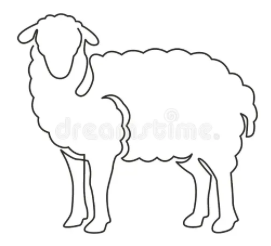
\includegraphics[height=0.6cm]{images/lamb1.png}
 \hspace{0em} 被恩典帶入榮耀 } 
 \fancyhead[RO]{
 \leftmark\hspace{0em} 
 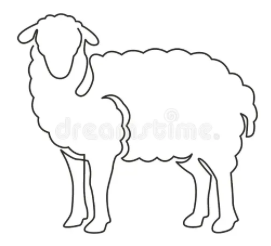
\includegraphics[height=0.6cm]{images/lamb1.png} 
} 
\fancyfoot[LE,RO]{\thepage} 
\renewcommand{\headrulewidth}{0pt}
\usepackage{fontawesome5}

%\titleformat{\chapter}
%  {\color{black}\Huge\bfseries} % format
%  {\thechapter}                    % 第 n 章
%  {1cm}                            % separation
%  {}
  
\begin{document}



\includepdf[
  pages=1,
  fitpaper=true,
  scale=1
]{cover/brought_into_glory_ebook_6_9.pdf}



% =========================
% Front Matter
% =========================

%\frontmatter
%\pagenumbering{arabic}

% ----- Copyright -----
\thispagestyle{empty}
\vspace*{\fill}
\footnotesize

\noindent
© 2026 Chris Kuo

\vspace{0.5cm}

\noindent 
%ISBN：\\
第一版：2026 年 12 月\\

本書任何部分不得以任何形式重製、儲存或傳播（包括電子、機械、影印、錄音或其他方式）。惟依據1976年《美國著作權法》第107條及第108條所規範之合理使用，或用於評論、教學及其他非商業性用途之適當引用，則不在此限。如有意以任何形式重製、儲存或傳播，請取得作者書面同意。

作者與出版者在編寫本書時，盡力求其內容準確與完整；然而，因人的有限，難免仍有疏漏之處。若讀者發現錯誤，懇請不吝指正。凡因使用本書內容所產生之任何結果，作者與出版者不承擔相關責任。
\vfill

\noindent The Innovation Press, \\
\noindent Ann Arbor, MI 
\begin{figure}[!htbp]
  
\includegraphics[width=0.20\textwidth]{others/innovation_press.png}% Replace example-image with the filename of your image
\end{figure}
\vfill


% ----- Copyright -----
\clearpage
\thispagestyle{empty}
\vspace*{\fill}
\normalsize{
\indent 親愛的\underline{\hspace{5cm}}：\\

\indent \indent 如果您偶爾會問天堂是怎麼樣子的，\\
\indent \indent 讓我邀請您來讀這本書！
}
\vspace*{\fill}




% ----- TOC -----
% ----- Front Matter -----
\pagenumbering{roman}

\clearpage
\addcontentsline{toc}{chapter}{啟示錄給你的福音}
\begin{center}
\begin{tcolorbox}[
    width=0.95\textwidth,
    colback=white, %gray!5,
    colframe=gray!70,
    colbacktitle=gray,
    coltitle=white,
    title={\small{\centering 你知道啟示錄中，有許多神要告訴你的福音嗎？}},
    fontupper=\small\setstretch{1.0},
    enhanced,
    boxrule=0.5pt,
    breakable,
    left=3pt,
    right=3pt,
    top=6pt,
    bottom=6pt
]

一、你是神所造的，你在祂眼中是寶貴的

你的生命不是偶然。神創造萬有，祂照著自己尊貴的形象造了你，賦予你任何人都奪不走的尊嚴。你被造，是為了認識祂。
\begin{ScriptureBox}
\item[4:11] 我們的主，我們的神，你是配得榮耀、尊貴、權柄的；因為你創造了萬物，並且萬物是因你的旨意被創造而有的。
\end{ScriptureBox}

\vspace{0.3cm}
二、耶穌愛你，並捨命救贖你

在啟示錄講到審判之前，它先讓我們看見一位救主。神的羔羊耶穌基督愛我們。祂捨了自己的生命，用自己的寶血，從各國各族中把人買回來歸於神。這也包括你。
\begin{ScriptureBox}
\item[1:5] 他愛我們，用自己的血使我們脫離罪惡。
\item[5:9] 因為你曾被殺，用自己的血從各族、各方、各民、各國中買了人來，叫他們歸於神。
\end{ScriptureBox}

\vspace{0.3cm}
三、我們為什麼需要祂

我們需要救贖主，因為每一個人都偏離了神。我們常常活得好像自己屬於自己，讓美好的事物佔據了唯獨屬於神的位置；我們甚至看不見自己有多貧窮。有一天，每個人的一生都要在神面前展開，我們的善行也無法洗去罪的責任。然而，主告訴我們這些，不是要壓垮我們，而是因為祂愛我們，盼望我們回到祂身邊。
\begin{ScriptureBox}
\item[3:17] 你說：我是富足，已經發了財，一樣都不缺；卻不知道你是那困苦、可憐、貧窮、瞎眼、赤身的。
\item[3:19] 凡我所疼愛的，我就責備管教他；所以你要發熱心，也要悔改。
\item[20:12] 死了的人都憑著這些案卷所記載的，照他們所行的受審判。
\end{ScriptureBox}

\begin{itemize}[leftmargin=2em, labelsep=0.3em]
\item[Q.] \AskItem{你是否感覺到，你與創造你的神之間少了些什麼，而你需要祂的赦免？}
\end{itemize}

\vspace{0.3cm}
四、今天就來到祂面前

\begin{ScriptureBox}
\item[7:14] 他們曾用羔羊的血把衣裳洗白淨了。
\item[3:20] 我站在門外叩門，若有聽見我聲音就開門的，我要進到他那裏去，我與他，他與我一同坐席。
\item[22:17] 來！聽見的人也該說：來！口渴的人也當來；願意的，都可以白白取生命的水喝。
\item[21:4] 神要擦去他們一切的眼淚；不再有死亡，也不再有悲哀、哭號、疼痛，因為以前的事都過去了。
\end{ScriptureBox}

人能夠站在神面前，不是因為從未犯過罪，而是因為他們知道用羔羊的血把污穢的心洗潔淨了。
你不需要先把自己變得夠好。基督已經在叩你的門。你可以照著你本來的樣子來：向祂承認你的罪，回轉歸向祂，相信耶穌為你受死並且復活。救恩是祂白白賜給你的禮物。

\vspace{0.3cm}

%\begin{itemize}[leftmargin=2em, labelsep=0.3em]
%\item[Q.] \AskItem{今天你願意接受神的恩典的邀請嗎？
%如果你願意，可以用自己的話，或跟著以下的內容禱告：}
%\end{itemize}

今天你願意接受神的恩典的邀請嗎？
如果你願意，可以用自己的話，或跟著以下的內容禱告：

\begin{tcolorbox}[
    width=\linewidth,
    colback=gray!5,
    colframe=gray!70,
    colbacktitle=gray!90,
    coltitle=white,
    title={決志禱告},
    center title,
    boxrule=0.5pt,
    breakable,
    left=1pt,
    right=1pt,
    top=1pt,
    bottom=1pt
]
親愛的天父：

\hspace{0.5cm} 謝謝你創造了我，也愛我。我承認我偏離了你，常常以自己為中心，得罪了你。求你赦免我的罪。 
主耶穌，我相信你是神的兒子，你為我流血捨命，又從死裏復活。

\hspace{0.5cm} 現在我打開心門，接受你作我的救主和生命的主。求你進到我心裏，用你的寶血洗淨我，使我成為你的兒女。
求聖靈引導我，使我一生跟隨你、敬拜你，直到那日與你同在新天新地之中。
 
\hspace{0.5cm} 奉主耶穌基督的名禱告，阿們！
\end{tcolorbox}


\end{tcolorbox}
\end{center}

\clearpage
\vspace*{-1.1in}
{
\setstretch{1.2}
\tableofcontents
}
\makeatletter
\clearpage
\vspace*{-1.1in}
%\addcontentsline{toc}{chapter}{表目錄}
{%
\setlength{\cftafterlottitleskip}{1em}   % space below 表目錄
  \setstretch{1.0}%
  \setlength{\cftbeforetabskip}{0.3em}%   same as \cftbeforechapskip in the TOC
  \let\addvspace\@gobble
  \listoftables
}
\vspace*{-1cm}
{%
\setlength{\cftafterloftitleskip}{1em}   % space below 圖目錄
  \setstretch{1.0}%
  \setlength{\cftbeforefigskip}{0.3em}%
  \let\addvspace\@gobble
  \let\clearpage\relax
%  \addcontentsline{toc}{chapter}{圖目錄}
  \listoffigures
}
\makeatother

% Main Matter
%\mainmatter
%\pagenumbering{arabic}

% Main Matter
\clearpage
\pagenumbering{arabic}


\chapter*{前言}
\addcontentsline{toc}{chapter}{前言}
\markboth{前言}{前言}


\section*{為什麼要邀請你讀這本書？}
\normalsize
也許你從來沒有聽過啟示錄，或許你知道啟示錄是聖經的最後一本書卷，可是懷疑它的真實性。也許你常常讀聖經，只是對啟示錄比較陌生。
如果你正有這樣的疑問，那這本書是專門爲你而寫的。

如果你未接觸基督信仰，你可能會以為啟示錄只是給基督徒讀的。可是我想告訴你，啟示錄是神自己邀請你來認識祂的福音的書。約翰寫下啟示錄之後，啟示錄就在小亞細亞眾教會中流傳開來。許多基督徒在壓力與逼迫之下，仍然持守信仰，甚至為基督作見證直到犧牲性命。這些早期基督徒所相信的，是一位真實來到世上的基督。

\section*{寫作動機—為什麼要寫這本書？}

因為關於末世預言的電影很多，也有不少電影和動畫以末世為背景，使人對啟示錄所描繪的世界產生好奇。因此，有些人也會翻閱啟示錄，想看看聖經究竟有沒有記載「世界末日會發生什麼事」。曾經有一位青少年告訴我，他讀聖經的目的，就是想看看裡面到底有沒有記載世界末日會發生什麼事。
 
當基督徒閱讀啟示錄時，我們的焦點也可能落在如何解釋龍、獸、印記、千禧年等問題上。其實，這也是我自己閱讀啟示錄時所經歷的一個轉折。因此，我寫這本書，是希望與讀者重新走進啟示錄。不是先從每一個單一事件開始，而是從耶穌基督開始。啟示錄的第一句話，不就是「耶穌基督的啟示」嗎？它是耶穌自己對你我說話。它讓我們知道，祂掌管歷史，祂審判邪惡，祂勝過撒但與死亡，祂再來，祂更新萬有，最後把祂所救贖的百姓帶入永恆的榮耀。

同時，我也盼望這本書能成為協助主日學教師的材料。因此，我盡量交代經文的背景與信息。盼望無論是個人靈修、小組查經，或教師教學，都能藉此一同思想啟示錄所見證的耶穌基督。

\section*{基督／羔羊是中心—如何讀啟示錄？}

當你翻閱啟示錄時，可能會很困惑，耶穌不是人嗎？怎麼就變成羔羊了？
這正是我們需要認識聖經整體的地方。耶穌第一次來，是贖罪的羔羊，祂被人類想出來最殘酷的刑罰，被釘在十字架上。這是他主動的行為，為了贖回在罪中被綑綁的人。我們哪裡知道祂是為我們的過犯而受害呢？聖經的《以賽亞書》（約是耶穌來到地上前700年），早已預言祂的代死。祂為我們的罪孽壓傷，「因祂受的刑罰，我們得平安；因祂受的鞭傷，我們得醫治。」（以賽亞書53:5）原來祂像是一隻羊羔被獻祭。

然而故事就此結束了嗎？沒有。啟示錄接續了耶穌的故事。祂以羔羊的身份來到，但如今是站立得勝的羔羊，並且是領軍的君王，我們也可以認得祂，因為祂穿著濺了血的衣服。（啟示錄19:13）所以啟示錄是一個以基督為中心的故事。祂掌權，展開書卷，審判邪惡，擊敗撒但，並且將祂所救贖的百姓帶入新創造的榮耀。

歷世歷代數不清的基督徒何其有幸，能被恩典帶入神的榮耀裡。相信正在讀本書的你也是其中大蒙恩典的一位，並且希望你看完此書之後，願意接受主恩典的邀請。

\section*{書名：「被恩典帶入榮耀」}

此書承襲《被恩典追上》的命名：人先被神的恩典追上，繼而被神的恩典改變，最後被神的恩典帶入祂的榮耀。因此，這一系列的名稱回應了一個蒙恩得救的基督徒所走的道路：
\begin{itemize}
\item 「被恩典追上」
\item 「被恩典改變」
\item 「被恩典帶入榮耀」
\end{itemize}
此書封面的「恩典」二字是紅色，象徵耶穌基督的寶血帶我們進入祂的榮耀裡。
那麼，為什麼要先寫第三部《被恩典帶入榮耀》呢？因為\textbf{知道終點，才能更清楚地知道改變的目的。}神在基督裡的救恩有一個榮耀的終點，就是使我們最終與基督同得榮耀。
當我們知道自己將往哪裡去，就更能明白今天為什麼需要被神改變。這正是保羅在《羅馬書》8章所描繪的救恩金鏈：

\begin{quote}
「因為祂\textbf{預先所知道}的人，就『預定』效法祂兒子的模樣，使祂兒子在許多弟兄中作長子。預先所定下的人又『召』他們來；所召來的人又『稱他們為義』；所稱為義的人又叫他們『得榮耀』。」—羅馬書 8:29-30
\end{quote}
從預定、呼召、稱義，到最終的得榮耀，這條救恩的道路不是人自己走向榮耀，而是神以祂的恩典一路帶領祂所救贖的人，直到榮耀的終點。

\section*{研究脈絡與主要著作}

歷來對啟示錄的研究卷帙浩繁，我在準備這本導讀性質的書時，只能有所選擇。
本書除了參考多位解經家與學者的研究，也整理了我過去研讀啟示錄以及教導主日學時所累積的資料與心得。
並在這次重新整理的過程中，我有許多新的發現及收穫，使我對啟示錄的基督，有了更深一層的認識。

以下幾位作者的書是我寫此書的參考重點：
\begin{enumerate}
\item John MacArthur（約翰. 麥克阿瑟）{\footnotesize\footnote{MacArthur, J. (2007). \textit{Because the Time Is Near: John MacArthur Explains the Book of Revelation}. Moody Publishers.}} —他的逐段解經，以及他對基督再來、基督掌權與最終得勝的論述。

\item Grant R. Osborne（格蘭特. 奧斯本）\footnote{Osborne, G. R. (2002). \textit{Revelation}. Baker Academic.} —他對不同啟示錄解讀的探討，幫助我從不同角度思考本書的象徵、結構與末世論主題。
    
\item G. K. Beale（G. K.\ 比爾）\footnote{Beale, G. K. (1999). \textit{The Book of Revelation: A Commentary on the Greek Text}. Wm. B. Eerdmans Publishing Co.} —他對舊約背景的廣泛研究，幫助我將啟示錄放在整體聖經故事中來理解，並看見其中豐富的舊約意象與神學脈絡。
    
\item Craig R. Koester（克雷格. 科斯特）\footnote{Koester, C. R. (2014). \textit{Revelation: A New Translation with Introduction and Commentary}. Yale University Press.} —他對啟示錄歷史背景與文學脈絡，使我更能理解這卷書向最初眾教會所傳達的信息。
    
\item Richard Bauckham（理查. 鮑坎）\footnote{Bauckham, R. (1993). \textit{The Theology of the Book of Revelation}. Cambridge University Press.} 
—他從神學角度的研究，幫助我進一步思考許多核心主題。
\end{enumerate}

這些作者各有不同的貢獻以及詮釋。因此，我盡力地呈現主要的不同觀點。本書的目的，是以容易理解的方式帶領讀者認識啟示錄，同時始終把它的核心聚焦在耶穌基督的得勝，以及祂的百姓最終進入永恆的榮耀。\footnote{
我也感謝吳榮滁牧師所開發的「新約引用舊約分析平台」，彷彿是神學院的教授在我旁指導，並使我查考的時間，事半功倍。https://chatgpt.com/g/g-69e26d759c108191ba873085c5722e4c-xin-yue-yin-yong-jiu-yue-fen-xi-ping-tai-nt-ot-citation-analyzer

我並感謝蘇桂村牧師二十多年來亦師亦友的陪伴與代禱。在他各地講道百忙之中，他仍願意逐頁讀我的寫作，提出許多寶貴的意見與建議，使我獲益良多。對於他的耐心與付出，我深表感謝。

當然，本書若有任何內容上的錯誤或疏漏，仍由我本人負全部責任。
}

\section*{表格與時間線：協助快速閱讀}

啟示錄包含豐富的異象與神學主題。為了幫助現代讀者理解並掌握這些豐富的內容，凡是可以清楚地透過表格或時間線呈現的資訊，我都盡量以這樣的方式加以整理。

如此一來，正文的討論就可以持續聚焦於耶穌基督的掌權、得勝，以及祂最終更新萬有的工作。對於經文中不同的解釋觀點，我在註腳或是附錄中加以說明。

\section*{本書的插圖：進入啟示錄的異象}

啟示錄充滿豐富而鮮明的圖像：龍、獸、羔羊、金燈臺、號筒、印、碗，以及新耶路撒冷等。對現代讀者而言，這些異象若只透過文字描述，有時不容易形成具體的畫面。因此，本書適度加入相關插圖，幫助讀者更直觀地掌握經文中的場景與信息。

雖然插圖的構思與製作需要投入不少時間，但若能幫助弟兄姊妹更深入地進入經文所呈現的異象，這些努力便是值得的。

然而，插圖也可能影響讀者對異象的想像，甚至加入經文未明確提供的細節。為此，本書的插圖盡量保持簡潔，主要發揮視覺輔助的作用，而不取代經文本身的描述與解釋。\footnote{本書的插圖由作者用 Google Gemini 反覆修改製作而定稿，並經過作者進一步的審閱、編輯與篩選。}

讀者應當以啟示錄的經文為依據，將插圖視為理解人物、場景與信息的輔助工具，而非解釋經文的權威。


\section*{結語}

寫完初稿時，我的心情是敬畏的。我這個蒙恩得救的人，竟要盡力寫出祂的榮耀。祂慈愛的大光照著我，使我的筆快活如馬，廢寢忘餐；可是，我這支不達意的筆，在我的造物主面前，又笨拙不如烏鴉一聲驚叫。

然而，我的造物主是知道的。祂知道我筆下所要述說的，是那位我所愛、所敬拜、所仰望的主。正如使徒約翰在啟示錄最後所說的：

\begin{quote}
「主耶穌啊，我願你來！」
\end{quote}

\vspace{2em}

\begin{flushright}
主僕  \\
郭景光弟兄\\
紐約新城歸正教會長老  \\
紐約州艾姆赫斯特
\end{flushright}
\chapter{認識榮耀的基督（1:1-1:11）}

你在四福音書中所認識的耶穌，是怎樣的一位耶穌呢？
那是祂第一次來到地上。祂謙卑地來到我們中間，祂服事人，醫治病患，尋找失喪的人，祂並且「捨命作多人的贖價」。
許多天主教堂裡的耶穌形象，是釘在十字架上的耶穌。祂頭戴荊棘的冠冕，身上滿是鞭傷。祂是受苦、受死的耶穌。我們很難與想像中的「榮耀」聯繫在一起。

這是什麼原因呢？使徒保羅告訴我們，原來祂是本有神榮耀的形像的，可是他「卻虛己，取了奴僕的形像，存心順服，以至於死，且死在十字架上。」（腓立比書2:6–8）

但故事並沒有停在十字架上。「神將他升為至高，又賜給他那超乎萬名之上的名，叫一切在天上的、地上的、和地底下的，因耶穌的名，無不屈膝。」（腓立比書2:9-10）
這正是啟示錄要我們看見的榮耀的基督。

啟示錄一開始，就是榮耀的基督說話。

\begin{ScriptureBox2}{圈出1:4–8中所有用來稱呼耶穌基督的名字和稱號。1:3向念這預言、聽見並遵守的人應許了什麼？}

\item[1:1] 耶穌基督的啟示、就是　神賜給他、叫他將必要快成的事指示他的眾僕人．他就差遣使者、曉諭他的僕人約翰．

\item[1:2] 約翰便將　神的道、和耶穌基督的見證、凡自己所看見的、都證明出來。

\item[1:3] 念這書上預言的、和那些聽見又遵守其中所記載的、都是有福的．因為日期近了。

\item[1:4] 約翰寫信給亞西亞的七個教會．但願從那昔在今在以後永在的　神．和他寶座前的七靈．

\item[1:5] 並那誠實作見證的、從死裡首先復活、為世上君王元首的耶穌基督．有恩惠平安歸與你們。他愛我們、用自己的血使我們脫離罪惡．〔脫離有古卷作洗去〕

\item[1:6] 又使我們成為國民、作他父　神的祭司．但願榮耀權能歸給他、直到永永遠遠。阿們。

\item[1:7] 看哪、他駕雲降臨．眾目要看見他、連刺他的人也要看見他．地上的萬族都要因他哀哭。這話是真實的。阿們。

\item[1:8] 主　神說、我是阿拉法、我是俄梅戛、〔阿拉法俄梅戛乃希臘字母首末二字〕是昔在今在以後永在的全能者。

\item[1:9] 我約翰就是你們的弟兄、和你們在耶穌的患難、國度、忍耐裡一同有分．為　神的道、並為給耶穌作的見證、曾在那名叫拔摩的海島上。

\item[1:10] 當主日我被聖靈感動、聽見在我後面有大聲音如吹號說、

\item[1:11] 你所看見的、當寫在書上、達與以弗所、士每拿、別迦摩、推雅推喇、撒狄、非拉鐵非、老底嘉、那七個教會。

\end{ScriptureBox2}

\begin{ReaderQuestion}
如果我們知道將來要與基督一同作王、在神面前事奉，今天應當如何活出屬祂的身分？
\end{ReaderQuestion}

\section{啟示錄是約翰在拔摩島上記的}

約翰寫了約翰福音、約翰一書、約翰二書和約翰三書。
後來約翰在羅馬皇帝統治期間，因為基督信仰和為基督作見證而被放逐到拔摩海島。在島上記載了這卷啟示錄。
見圖\ref{fig:turkey-seven-churches}：
\ding{172}以弗所、\ding{173}士每拿、\ding{174}別迦摩、\ding{175}推雅推喇、\ding{176}撒狄、\ding{177}非拉鐵非、\ding{178}老底嘉。圈＝拔摩島。

\begin{figure}[htbp]
    \centering
    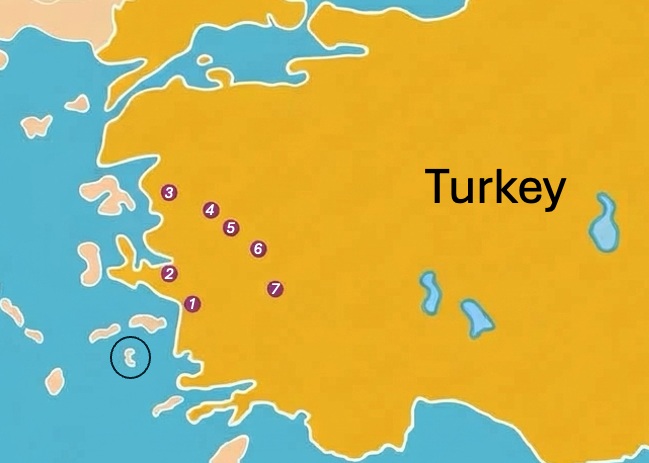
\includegraphics[
        width=0.9\textwidth,
        trim=0 0 0 100,
        clip
    ]{images/turkey}
    \caption{啟示錄七個教會的位置}
    \label{fig:turkey-seven-churches}
\end{figure}

在那孤獨、患難的環境中，他所看見的這些異象，會不會只是他的幻覺？
不是的。原因有二。第一，約翰並不是失去意識下而寫的。當異象出現時，他常常知道自己正在看見什麼，也記錄了天使對他的解釋。他甚至提出問題，並得到回答。
第二，啟示錄也是可靠的紀錄。第二世紀的教父愛任紐（Irenaeus）在《駁異端》（Against Heresies）中多次引用啟示錄。\footnote{
Irenaeus. (1885). \textit{Against heresies} (A. Roberts \& W. H. Rambaut, Trans.). Christian Literature Publishing. (Original work published ca. 180)}
愛任紐距離使徒約翰的時代並不遠。
到了第四世紀，史學家優西比烏（Eusebius）在《教會史》中整理早期教會傳統。他記載了約翰、拔摩以及圖密善時期的相關傳統。\footnote{
Eusebius. (1890). \textit{Church history} (A. C. McGiffert, Trans.).
Christian Literature Company. (Original work published ca. 325)}
優西比烏記載，約翰後來回到以弗所。\footnote{Eusebius, ca. 325/1885, 3.18.1, 3.20.9}
所以啟示錄是第一世紀真實流傳、保存並傳承的使徒見證。

啟示錄中的基督，是怎樣的基督呢？

\section{啟示錄中的榮耀基督}

如果你心中的耶穌是受苦的僕人，你更可以確定，祂原來是尊貴的君王。
新約歌羅西書 1:15 說「愛子是那不能看見之神的像」。希伯來書 1:3 也說「他是神榮耀所發的光輝，是神本體的真像」。
在啟示錄第一章到第三章中，我們看到許多關於耶穌的榮耀的描述。我們可以綜合成為表\ref{tab:christ-revelation-1-3}。

%\ref{fig:john_saw_christ_white.jpg}

{
\setstretch{1.0}
\begin{longtable}{p{1.6cm} p{7.3cm}}
\caption{啟示錄一至三章中對基督的形容}
\label{tab:christ-revelation-1-3} \\
\toprule
\textbf{經文} & \textbf{耶穌基督的形容} \\
\midrule
\endfirsthead

\toprule
\textbf{經文} & \textbf{耶穌基督的形容} \\
\midrule
\endhead

\bottomrule
\endfoot

\bottomrule
\endlastfoot

1:5
& 從死裡首先復活 \\
\midrule[0.2pt]
3:14
& 祂在一切受造之上，並超越地上的君王。 \\
\midrule[0.2pt]
1:8
& 祂是初，也是終；祂超越時間，掌管歷史。 \\
\midrule[0.2pt]
1:13
& 祂是真正的人類中的一位。祂身穿長衣，直垂到腳，胸間束著金帶。顯出祂尊貴、君王與祭司的身分。 \\
\midrule[0.2pt]
1:14
& 頭與髮皆白，如白羊毛，如雪。象徵聖潔與尊貴。是但以理書中的「亙古常在者」。 \\
\midrule[0.2pt]
1:14; 2:18
& 眼目如同火焰。祂洞察人心，察驗人的內心，無一事能在祂面前隱藏。 \\
\midrule[0.2pt]
1:15; 2:18
& 腳好像在爐中鍛鍊光明的銅；腳像光明銅的。象徵力量、純潔與公義的審判。 \\
\midrule[0.2pt]
1:15
& 聲音如同眾水的聲音，帶著威嚴與權柄。 \\
\midrule[0.2pt]
1:16; 2:1; 3:1
& 右手拿著七星；在七個金燈臺中間行走；有神的七靈和七星的。祂掌管教會，也在教會中間行走、察看，並掌管聖靈的工作。 \\
\midrule[0.2pt]
1:16; 2:12
& 從祂口中出來一把兩刃的利劍；那有兩刃利劍的。祂以真理審判錯謬與罪惡，也以祂的話語勝過仇敵。 \\
\midrule[0.2pt]
1:16
& 面貌如同烈日放光。顯明祂的尊貴與神聖。 \\
\midrule[0.2pt]
1:18
& 拿著死亡和陰間的鑰匙。 \\
\midrule[0.2pt]
3:7
& 拿著大衛的鑰匙。祂擁有大衛君王的權柄，開了就沒有人能關。 \\
\midrule[0.2pt]
3:14
& 誠信真實見證的。祂是完全可靠、真實的見證。 \\
\end{longtable}
}

\begin{ReaderQuestion}
在表\ref{tab:christ-revelation-1-3}中，圈出那些與你平常心中耶穌形象不同的字詞。這表中的基督，與你心中的形象有什麼不同？
\end{ReaderQuestion}

\section{舊約早已預告基督的榮耀}
\label{sec:ch01_ot}

而且，約翰所描述的榮耀基督，與舊約先知在數百年前所看見的異象非常相似。
這不是巧合。熟讀舊約的猶太人讀到啟示錄中的基督，就會認出祂正是舊約所預告、所盼望的那位榮耀君王。
\begin{itemize}
\item 但以理書7:9：「我觀看、見有寶座設立、上頭坐著亙古常在者、他的衣服潔白如雪、頭髮如純淨的羊毛、寶座乃火焰、其輪乃烈火．」
\item 但以理書7:13：「我在夜間的異象中觀看、見有一位像人子的、駕著天雲而來、被領到亙古常在者面前。」
\item 但以理書7:14：「得了權柄、榮耀、國度、使各方各國各族的人都事奉他．他的權柄是永遠的、不能廢去、他的國必不敗壞。」
\item 但以理書10:6：「他身體如水蒼玉、面貌如閃電、眼目如火把、手和腳如光明的銅、說話的聲音如大眾的聲音。」
\item 以西結書43:2：「以色列　神的榮光從東而來．他的聲音如同多水的聲音．地就因他的榮耀發光。」
\item 以賽亞書22:22：「我必將大衛家的鑰匙放在他肩頭上．他開、無人能關．他關、無人能開。」
\end{itemize}
這些先知都曾在艱難的時代中看見基督的榮耀。榮耀的主沒有忘記祂的僕人，反而向他們顯明自己的榮耀，成為他們的力量和盼望。

如果你心中的耶穌只有受苦、被棄絕、被釘十字架的一面，那麼你需要再次提醒自己：祂本有神的形象，也是已經復活、得勝、掌權的榮耀之主。

\begin{ReaderQuestion}
同一位基督曾取了奴僕的形象、為我們受苦、被棄絕並死在十字架上，如今卻坐在寶座上、掌管列國。這兩個面向如何幫助我們更完整地認識耶穌？
\end{ReaderQuestion}

因此，當我們認識這位榮耀的基督，就能在今天的苦難中仍然有盼望，在軟弱中仍然有力量，在黑暗中仍然忠心，直到祂再來。

\begin{ReaderQuestion}
當教會面對患難、逼迫、試探與軟弱時，認識基督是首先的、末後的、曾死過又活著、並且拿著死亡和陰間的鑰匙，如何幫助我們仍然忠心持守？
\end{ReaderQuestion}

\chapter{基督對祂的教會說話（2:1-3:13）}
\normalsize
\section{先了解初代教會的時代背景}

寫啟示錄的約翰所處的年代，正是羅馬帝國最強盛的時期之一。地上的君王，似乎無可匹敵。
也就在這個年代，初代教會誕生。他們認識真正的君王基督，並且為真理作見證，甚至至死不渝。

羅馬帝國高度集權，皇帝的權威遍及帝國各地。皇帝崇拜也逐漸成為帝國公共生活的一部分。不過，各地的宗教政策並不完全一致；只要不被視為威脅帝國秩序，許多民族仍可以保留自己的傳統宗教。猶太教歷史悠久，在羅馬統治下可以享有一定程度的宗教特權，因此猶太人通常可以按照祖先的律例敬拜上帝。基督教起初從猶太教的背景中發展出來，在一些地方也被視為猶太傳統中的一個群體；但隨著基督教逐漸與猶太教分離，這種既有的宗教身分的保護傘也就減弱了。\footnote{Beale, G. K. (1999).}

基督徒敬拜獨一真神，宣認耶穌基督是真正的主，因而不能把皇帝當作神來敬拜。這使他們遭受社會敵意與官方壓力，甚至在某些地區面臨財產被沒收、流放或處死的危險。

我畫出了西元1年至138年的皇帝時間軸。圖\ref{fig:roman_emperors}可以讓我們可以看見這段時期羅馬政權的更迭。
其中，尼祿（Nero）與圖密善（Domitian）在歷史上常被稱為暴君。兩人都集中皇權、壓制政敵、處決反對者，也曾以叛國罪等罪名打擊政敵。尼祿尤其因西元64年羅馬大火後迫害基督徒而聞名。
見表\ref{tab:nero-domitian-zh}。
\footnote{至於圖密善，古代資料記載他鎮壓異議者，但是否曾大規模地迫害基督徒，仍有不同看法。}



\begin{figure}[htbp]
    \centering
    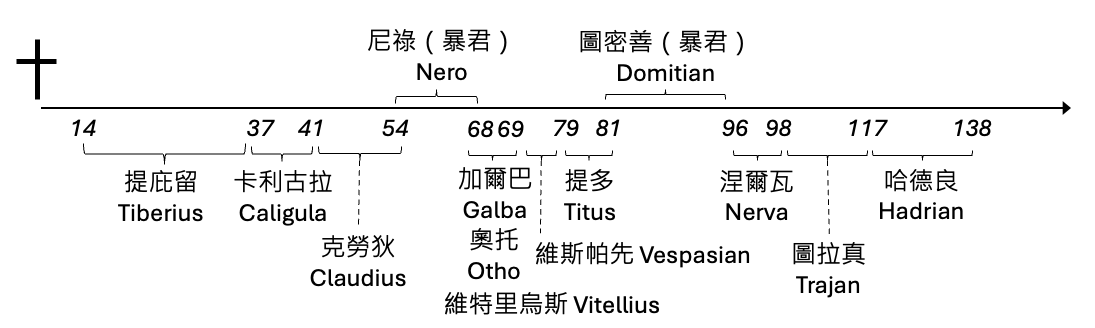
\includegraphics[width=\textwidth, trim=0 0 0 0, clip]{images/roman_emperors.png}
    \caption{西元1年至138年的羅馬皇帝時間軸}
    \label{fig:roman_emperors}
\end{figure}





\clearpage
{
\small
\begin{longtable}{|p{2.5cm} | p{6.5cm}|}
\caption{尼祿、圖密善} 
\label{tab:nero-domitian-zh} \\
\hline 
\textbf{人物} \footnote{此尼祿肖像現位於慕尼黑雕塑館，圖密善肖像現位於法國羅浮宮。} &
\textbf{迫害} \\
\hline
\centering
尼祿（Nero）\\
\includegraphics[
    width=\linewidth,
    trim=0 0 0 0, 
    keepaspectratio
]{images/nero.jpg}

&
\vspace{-0.3cm}
\begin{itemize}[nosep, leftmargin=10pt]
\item 處決政敵與元老院議員。
\item 以叛國罪等法律打擊政敵。
\item 下令殺害自己的母親阿格里皮娜（Agrippina）。
\item 羅馬大火（64 年）後迫害基督徒。
\item 以恐懼、暴力和專斷的手段統治。
\item 拒絕參與帝國崇拜者可以被控為「不敬神」（atheism）。
\end{itemize}
\\[-0.5cm]
\hline

\centering
圖密善\\
（Domitian）\\
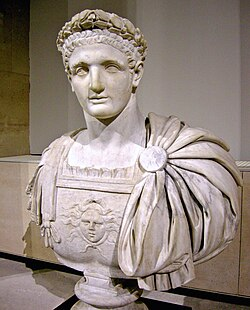
\includegraphics[
    width=\linewidth,
    keepaspectratio
]{images/domitian.jpeg}

&
\vspace{-0.3cm}
\begin{itemize}[nosep, leftmargin=10pt]
\item 處決元老院議員及政敵。
\item 以叛國罪等法律打擊政敵。
\item 沒收被定罪政敵的財產。
\item 要求以「主與神」（Dominus et Deus）稱呼他。此稱呼在書面和口頭上都不可更改。\footnote{Suetonius. (1914). Lives of the Caesars: Volume II (J. K. Rolfe, Trans.). Harvard University Press.}
\item 拒絕參與帝國崇拜者可以被控為「不敬神」（atheism）。
\item 透過猜疑、告密與壓制來統治。
\end{itemize} 
\\
\hline
\end{longtable}
} 

了解此逼迫嚴峻的時代，我們來讀耶穌給七個教會的書信。七個教會的位置，可以參照圖\ref{fig:turkey-seven-churches}。
\normalsize
\subsection{為什麼是此七間教會？}

讀者的第一個問題，可能是為什麼是此七間教會？新約書信還提到羅馬、哥林多、腓立比、歌羅西、帖撒羅尼迦等許多教會，怎麼沒有在其中？
這七間教會之所以出現在啟示錄中，並不是約翰自行挑選的，而是基督吩咐約翰的：「你所看見的，當寫在書上，達與亞細亞的七個教會」。
「七」是啟示錄中反覆出現、表達完整性的數字。因此，這七封書信不只是給這七間教會，每封書信最後都以「聖靈向眾教會所說的話，凡有耳的，就應當聽」作結。這表示基督對一間教會所說的話，也是在向眾教會說話。

為了讓讀者更貼近當時的處境，我特別設計了「弟兄對話」，讓我們彷彿走進這七間教會，在聽見基督說話以前，先聽見弟兄姊妹如何看待自己的教會，以及他們所處的環境。

這七封書信都有基督對各教會的稱許、責備、命令和應許。我也將基督的信息分為「基督的稱許」、「基督的責備」、「基督的命令」和「基督的應許」四個部分。
特別值得注意的是，其中有兩間教會的「基督的稱許」標示為「沒有」。「沒有」這兩個字何等令人警醒，也何等令人心痛。若主親自對我們的教會說話，我們是否也能聽見祂的稱許？還是我們也只能面對一個令人心痛的「沒有」？

\section{以弗所教會(2:1-7)}

\begin{DialogueBox}
\noindent\faUser\ 弟兄一：「我們以弗所的弟兄們，向來看重主的道。有人傳講異樣的教訓，我們便察驗；有人自稱使徒，我們也不輕易接納。這些年來，眾弟兄為主的名勞苦，忍耐逼迫，也沒有因患難退後。我想，我們既如此持守主的道，又忠心服事，求主悅納我們的工作。」

\noindent\faUser\ 弟兄二：「我們確實為主的名作了許多工。只是……我有時想起我們初信主的日子，那時弟兄姊妹熱切相愛，聽道、禱告、擘餅。如今我們仍然持守真道，也仍然殷勤作工，只是不知不覺間，我們裡面起初愛主、愛弟兄的心，是否已不如從前了？」
\end{DialogueBox}

\subsection{地理背景}
以弗所教會所在的以弗所城，是一座繁華而深受偶像崇拜影響的城市。
今天如果前往以弗所古城參觀，仍然可以看到以弗所大劇場、海港大道、大理石大道、古代市集廣場、圖書館、神殿與噴泉等遺址。走在這些保存至今的遺跡之間，我們仍能想像當年以弗所作為羅馬帝國重要城市之一的繁華景象。

以弗所的大亞底米神廟（Temple of Artemis）是以弗所城市身分的重要象徵。大亞底米（Artemis）是希臘名稱，羅馬人稱她為 Diana（戴安娜）。對亞底米的崇拜不只是宗教活動，也帶動了相關的商業與手工業。使徒行傳19:24記載，銀匠底米丟「為亞底米製造銀龕」，使許多工匠因此獲利。

然後保羅一行人在以弗所傳講福音，許多人離棄偶像歸向基督。福音的傳播改變了人的生命，因此也開始影響以偶像崇拜為中心的社會與經濟活動。於是，銀匠底米丟聚集其他銀匠和相關工匠，指控保羅一行人威脅亞底米的尊榮，使他們的生意受到影響。結果，整座城都轟動起來。眾人湧進大劇場，約有兩個小時不住地喊著：「大哉！以弗所人的亞底米啊！」
路加醫生也不減幽默，他記著：「聚集的人、紛紛亂亂、有喊叫這個的、有喊叫那個的、大半不知道是為甚麼聚集。」（使徒行傳19:28,32,34）

想像一下，當時眾人聚集在巨大的劇場中，持續兩個小時高聲呼喊。這不僅讓我們看見以弗所城市的規模，也讓我們感受到他們的宗教熱情，以及偶像崇拜在城市生活中的重要地位。

正是在這樣一座繁華、富庶，又深受偶像崇拜影響的城市中，基督建立了祂的教會。
以弗所教會是蒙受豐富恩典的教會。保羅給以弗所教會的書信，一開始就是偉大的揀選論：「神從創立世界以前、在基督裡揀選了我們。」（以弗所書1:4)並且說明神在基督裡所成就的偉大奧秘。
這奧秘就是教會。就是「外邦人在基督耶穌裡、藉著福音、得以同為後嗣、同為一體、同蒙應許。」（以弗所書3:6）。他更為他們禱告，使基督因他們的信住在他們心裡，使他們的愛心「有根有基」，並且「能以和眾聖徒一同明白基督的愛，是何等長闊高深」（以弗所書3:17–18）。以弗所教會知道神永恆的揀選，明白福音的奧秘，在基督裡得著豐富的恩典，也有信心和愛心。


\subsection{基督的稱許}

\begin{ScriptureBox}

\item[2:1] 你要寫信給以弗所教會的使者、說、那右手拿著七星、在七個金燈臺中間行走的、說、

\item[2:2] 我知道你的行為、勞碌、忍耐、也知道你不能容忍惡人、你也曾試驗那自稱為使徒卻不是使徒的、看出他們是假的來。

\item[2:3] 你也能忍耐、曾為我的名勞苦、並不乏倦。

\end{ScriptureBox}

這是一群身體力行的信徒。他們為主勞碌、忍耐，持守真道，分辨是非。保羅與他們告別時，以弗所教會眾長老流淚痛哭，最令眾長老傷心的，是保羅所說：「以後不能再見我的面」（使徒行傳20:38）。
保羅更鄭重的勸他們警醒，因為「必有兇暴的豺狼進入你們中間，不愛惜羊群」（使徒行傳20:29）。這是一群有真理、有勞苦、有忍耐，也有愛的信徒。

\subsection{基督的責備}

\begin{ScriptureBox}

\item[2:4] 然而有一件事我要責備你、就是你把起初的愛心離棄了。

\end{ScriptureBox}

然而，約三十多年後，基督透過約翰向這間教會說「你把起初的愛心離棄了。」

從第一代的基督徒，到此時，教會中可能已經有了第二、第三代的信徒。真理的教導，教會的事奉，和會眾忍耐的品格都在。從人的眼光來看，這真是眾教會的榜樣。
可是有一份元素漸漸在流逝了，那就是起初的愛。這正是以弗所教會最值得我們思想的地方：一間可以為真理站立、為主勞苦、忍耐到底的教會，仍然可能在不知不覺中失去起初的愛。

\subsection{基督的命令}

\begin{ScriptureBox}

\item[2:5] 所以應當回想你是從那裡墜落的、並要悔改、行起初所行的事．你若不悔改、我就臨到你那裡、把你的燈臺從原處挪去。

\item[2:6] 然而你還有一件可取的事、就是你恨惡尼哥拉一黨人的行為、這也是我所恨惡的。

\end{ScriptureBox}

冷淡了的愛心，如何回到最初？答案是：悔改。
悔改使冷淡的心重新被主喚醒，使失落的愛重新燃起。即使我們已經走了很遠的路，恩典仍然可以使我們回轉，使我們在主裡日新又新。
悔改不是單單為過去的失敗感到難過，而是重新轉向基督，回到起初愛祂、跟隨祂的生命。
我們需要天天悔改，就是主耶穌吩咐的，「天天背起自己的十字架來跟從我。」（路加福音 9:23）


值得注意的是，基督對以弗所教會的責備，並不表示他們在真理上已經妥協。相反地，他們仍然恨惡尼哥拉一黨人的行為，這一點也是基督所肯定的。關於「尼哥拉一黨」究竟是什麼人，我們今天並不能確定其具體背景與教導。 \footnote{MacArthur, J. (2007).} 然而，他們所代表的，是一種基督所恨惡的錯誤教導與行為。

\subsection{基督的應許}

\begin{ScriptureBox}

\item[2:7] 聖靈向眾教會所說的話、凡有耳的、就應當聽。得勝的、我必將　神樂園中生命樹的果子賜給他喫。

\end{ScriptureBox}

這裡的「生命樹」明顯把我們帶回創世記2–3章。而「樂園」對應啟示錄22:1–5。因此，從創世記到啟示錄，我們可以看見：人是從伊甸園的失落，到基督裡的救贖，到得勝者進入神的樂園，到新天新地中的完全同在。基督不只是呼召祂的教會在地上忠心到底；祂最終要把屬祂的人帶入榮耀裡。
今天教會所面對的爭戰、悔改、忍耐與忠心，都不是救贖故事的終點；終點乃是進入神永恆的同在。所以，基督給以弗所教會的應許，既回應了他們當下的光景，也把他們的眼目帶向最後的榮耀。

\section{士每拿教會(2:8-2:11)}

\begin{DialogueBox}
\noindent\faUser\ 弟兄一：「我們士每拿，按著世人的眼光看，是困苦貧窮的。有人因信主的緣故受人毀謗，有人因不肯隨從眾人去稱君王是神，而失去生計。已有弟兄為主的名捨了性命。然而，雖是如此，我們仍聚集在一起敬拜主。若能持守基督的名，地上的貧窮又算得甚麼呢？」

\noindent\faUser\ 弟兄二：「我們在世人眼中或許一無所有，但有一樣，是無論如何也不可失去的，就是對主的忠心。將來所要面對的苦楚，也許比今日更深；但我們既已歸屬基督，就當持守到底。」
\end{DialogueBox}

\subsection{地理背景}

士每拿，是今天土耳其第三大城市伊茲米爾（İzmir），也是愛琴海沿岸的重要港口城市。今日仍可看見許多不同時代留下的歷史痕跡，包括古代市集廣場（Agora），羅馬時期的柱廊、公共建築與城市基礎設施。

士每拿在羅馬時代，就是忠誠於羅馬的重要城市。早在主前約195年，士每拿便建立了獻給「羅馬」（Roma）的神廟，表達對羅馬的忠誠。到了主後26年，士每拿又在與其他亞洲城市的競爭中獲准建立獻給提比留皇帝、莉薇亞以及羅馬元老院的神廟。

在這樣的背景下，基督徒拒絕參與皇帝崇拜，就可能被視為拒絕履行忠誠。對士每拿的基督徒而言，心裡相信並口裡承認「耶穌是主」，是一個關乎生命的事情。所以我們更能了解主耶穌對士每拿教會的稱許是何等寶貴。



\subsection{基督的稱許}

\begin{ScriptureBox}

\item[2:8] 你要寫信給士每拿教會的使者說、那首先的、末後的、死過又活的說、

\item[2:9] 我知道你的患難、你的貧窮、（你卻是富足的）也知道那自稱是猶太人所說的毀謗話、其實他們不是猶太人、乃是撒但一會的人。

\end{ScriptureBox}

士每拿教會一直保持此至死忠心的優良美德。約在主後155–160年間，坡旅甲（Polycarp）是士每拿教會的監督，坡旅甲年輕時曾到以弗所，接受使徒約翰的教導。他被捕並被帶到官府面前。根據《坡旅甲殉道記》\footnote{\textit{Martyrdom of Polycarp}. (1885). (A. Roberts \& J. Donaldson, Trans.).
Christian Literature Publishing. (Original work published ca. 155)}，當他被要求否認基督時，他回答：「我服事祂八十六年，祂從未虧負我；我怎能褻瀆那拯救我的王？」他也是早期基督教最著名的殉道見證之一。士每拿是一座以忠於羅馬而聞名的城市；基督卻在這座城市中建立了一群只以基督為王的子民。

\subsection{基督的責備}

沒有。

\subsection{基督的命令}

\begin{ScriptureBox}

\item[2:10a] 你將要受的苦你不用怕．魔鬼要把你們中間幾個人下在監裡、叫你們被試煉．你們必受患難十日。你務要至死忠心、

\end{ScriptureBox}

這裡的十日，表明是一段短的日子。患難有期，非無限期並失控的苦難。

\subsection{基督的應許}

\begin{ScriptureBox}

\item[2:10b] 我就賜給你那生命的冠冕。

\item[2:11] 聖靈向眾教會所說的話、凡有耳的、就應當聽。得勝的、必不受第二次死的害。

\end{ScriptureBox}

「第二次的死」指的是末後的審判與永遠的刑罰（啟示錄20:14）。這裡的「得勝」，不是說信徒靠自己的忠心賺取救恩，而是指屬基督的人在患難中持守信仰，靠著基督的恩典忠心到底。
對士每拿教會而言，這個應許尤其寶貴。他們因忠於基督而殉道。但肉身的死亡並不能改變基督所賜的永恆生命。那位「死過又活的」基督已經勝過死亡，因此屬祂的人不受第二次死的害。他們可能失去今生的生命，卻不會失去基督所賜的永恆生命。

\section{別迦摩教會(2:12-2:17)}

\begin{DialogueBox}
\noindent\faUser\ 弟兄一：「別迦摩是何等繁盛的城，眾多神廟林立，祭祀之事日日不息。只是，城中的人設席祭祀，邀請我們同席，我們無法拒絕。是否只要守住所信的，其他稍作退讓，也可以吧？」

\noindent\faUser\ 弟兄二：「我也曾如此想過。有些弟兄說，只要心裡仍信靠基督，偶爾赴席、吃祭偶像之物，也可以。可是近來我心裡越發不安……我們原是蒙召離開偶像歸向主的。若一次又一次向這些事退讓，我們究竟是在保守自己，還是在一步一步偏離主的道呢？」
\end{DialogueBox}


\subsection{地理背景}

別迦摩（Pergamum）就是今天土耳其西部的貝爾加馬（Bergama），位於伊茲密爾省（Izmir Province），今日的古城遺址已列入世界文化遺產。今日來到貝爾加馬，可以看到別迦摩的衛城（Acropolis），位於山丘頂端，可以看到古代劇場、雅典娜神廟、圖書館、宙斯祭壇遺址，以及羅馬帝國君王圖拉真神廟。阿斯克勒庇翁（Asclepion）：古代著名的醫療與治療中心，也是別迦摩最重要的羅馬時期遺址之一。別迦摩以圖書館與羊皮紙（parchment）聞名，是古代重要的知識中心。它羅馬時期則成為亞細亞行省的重要城市，並具有帝國崇拜中心的功能。

\begin{figure}[htbp]
    \centering
    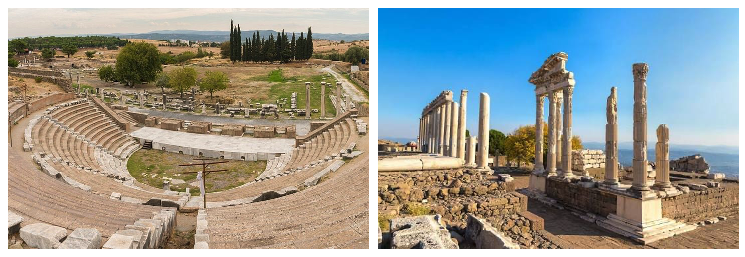
\includegraphics[
    width=1\textwidth, 
    trim=0 0 0 0, 
    clip]{images/pergamum3.png}
    \caption{別迦摩古代劇場、宙斯祭壇遺址}
    \label{fig:pergamum3}
\end{figure}

\subsection{基督的稱許}

\begin{ScriptureBox}

\item[2:12] 你要寫信給別迦摩教會的使者、說、那有兩刃利劍的說、

\item[2:13] 我知道你的居所、就是有撒但座位之處．當我忠心的見證人安提帕在你們中間、撒但所住的地方被殺之時、你還堅守我的名、沒有棄絕我的道。

\end{ScriptureBox}

別迦摩不只是文化與知識的中心，也是一座具有濃烈宗教與帝國崇拜氣氛的城市。 因此，2:13稱為「有撒但座位之處」。

\subsection{基督的責備}

\begin{ScriptureBox}

\item[2:14] 然而有幾件事我要責備你、因為在你那裡、有人服從了巴蘭的教訓．這巴蘭曾教導巴勒將絆腳石放在以色列人面前、叫他們喫祭偶像之物、行姦淫的事。

\item[2:15] 你那裡也有人照樣服從了尼哥拉一黨人的教訓。

\end{ScriptureBox}

在民數記25章，巴蘭引誘以色列人與摩押女子發生不正當的性淫亂，和陷入偶像崇拜，使他們得罪神。

以色列人在異教環境中，因為妥協而陷入偶像崇拜與淫亂。所以這裡是在告訴別迦摩教會，你們現在所面對的問題，並不是一個全新的問題。
這個問題以色列在曠野曾經面對過，而你們正在重演那個故事。
應用在今日，這如同是「妥協性的教導和門徒訓練」。是我們應當謹慎的。

\subsection{基督的命令}

\begin{ScriptureBox}

\item[2:16] 所以你當悔改、若不悔改、我就快臨到你那裡、用我口中的劍、攻擊他們。

\end{ScriptureBox}
如第一章表\ref{tab:christ-revelation-1-3}，基督口中利劍代表祂以真理審判錯謬。所以這裡是呼召教會離開錯誤的教導和行為，重新忠於基督。

\subsection{基督的應許}

\begin{ScriptureBox}

\item[2:17] 聖靈向眾教會所說的話、凡有耳的、就應當聽。得勝的、我必將那隱藏的嗎哪賜給他．並賜他一塊白石、石上寫著新名．除了那領受的以外、沒有人能認識。

\end{ScriptureBox}

嗎哪首先讓人想到以色列人在曠野中所吃的嗎哪（出埃及記16:15）。別迦摩教會在這個充斥異教崇拜的敵對環境，基督卻應許得勝者有另一種「食物」。不是向偶像妥協所得到的東西，而是從基督而來的真正生命供應。

這裡「白石」最好的理解似乎是按照羅馬人的習俗來解釋這塊「白石」。在競技比賽中，勝利者會獲頒白石。白石上刻有運動員的名字，並作為他參加特別頒獎宴席的入場券。\footnote{MacArthur, J. (2007). }
「新名」在聖經裡常常涉及新的身分、與神新的關係，所以，這裡的應許是，忠於基督的人，基督要以更深的生命供應和新的身分來代替。

\section{推雅推喇教會(2:18-29)}

\begin{DialogueBox}
\noindent\faUser\ 弟兄一：「我們推雅推喇的弟兄姊妹，殷勤服事，彼此相愛，又有信心和忍耐。近來開辦的慈善事工，也比從前更加增長。我們又透過參與城中各行各業的聚會，積極傳福音、幫助鄰舍。我想，只要我們一面持守對主的忠心，一面與眾人和睦相處，豈不是也能在這城中為主作美好的見證嗎？」

\noindent\faUser\ 弟兄二：「我也盼望如此。只是，有些事情實在叫我心裡不安。各行各業聚會的時候，常常會有向偶像獻祭的事情。我們教會甚至邀請那個自稱為先知的婦人耶洗別來教導。她勸說，信徒也可以吃祭偶像之物。」
\end{DialogueBox}


\subsection{地理背景}

推雅推喇（Thyatira／Thyateira）位於今天的土耳其西部的阿克希薩爾（Akhisar）。它不是以宏偉的政治地位或大型宗教中心聞名，而是以商業和手工業著稱。考古發現顯示，推雅推喇有非常多不同的行會（guilds），包括羊毛工人，染布工人，亞麻工人，皮革工人，銅匠等等。使徒行傳16:14 中的呂底亞（Lydia）就是一個賣紫色布匹的推雅推喇城的人。她在腓立比遇到保羅，後來成為基督徒。這些行會不只是單純的職業協會，同時也具有社交、向城市的神明獻祭或宗教宴席。此地行會工藝精湛，「腳像光明的銅」正可能是引用當地的銅匠的銅藝。這裡的銅，是一種由銅與鋅混合而成的合金，是一種較為純淨、精煉的黃銅。推測這類金屬是由推雅推喇（Thyatira）當地的工匠行會為軍事用途所製造。\footnote{Osborne, G. R. (2002).}

\subsection{基督的稱許}

\begin{ScriptureBox}

\item[2:18] … 那眼目如火焰、腳像光明銅的　神之子、說、

\item[2:19] 我知道你的行為、愛心、信心、勤勞、忍耐．又知道你末後所行的善事、比起初所行的更多。

\end{ScriptureBox}

\subsection{基督的責備}

\begin{ScriptureBox}

\item[2:20] 然而有一件事我要責備你、就是你容讓那自稱是先知的婦人耶洗別教導我的僕人、引誘他們行姦淫、喫祭偶像之物。

\item[2:21] 我曾給他悔改的機會、他卻不肯悔改他的淫行。

\item[2:22] 看哪、我要叫他病臥在床、那些與他行淫的人、若不悔改所行的、我也要叫他們同受大患難。

\item[2:23] 我又要殺死他的黨類、〔黨類原文作兒女〕叫眾教會知道、我是那察看人肺腑心腸的．並要照你們的行為報應你們各人。

\end{ScriptureBox}

耶洗別是北國以色列王亞哈的外邦王后，積極推動巴力崇拜、逼迫耶和華的先知，並因悖逆上帝而成為聖經中邪惡與淫亂的象徵。（列王紀上17–21章）。約翰刻意把一個當代教會中的人物稱為「耶洗別」，使讀者透過舊約人物來理解當前教會的問題。
這裡的「行姦淫、喫祭偶像之物」包括實際的異教祭祀以及社會生活中的宴席。在舊約中，「淫亂」又經常成為以色列背離耶和華、追隨偶像的象徵語言。
因此，這段經文的核心問題是教會是否仍然忠於基督，還是為了與周圍的文化、宗教、權力結合而妥協？

\subsection{基督的命令}

\begin{ScriptureBox}

\item[2:24] 至於你們推雅推喇其餘的人、就是一切不從那教訓、不曉得他們素常所說撒但深奧之理的人．我告訴你們、我不將別的擔子放在你們身上。

\item[2:25] 但你們已經有的、總要持守、直等到我來。

\end{ScriptureBox}
這裡的「撒但深奧之理」有兩種可能的解釋：\footnote{Osborne, G. R. (2002); Beale, G. K. (1999).}
\begin{enumerate}
\item 諷刺性的說法：這可能是在諷刺耶洗別所聲稱自己「知道神深奧之事」（參歌林多前書 2:10）。
\item 按字面理解：耶洗別可能是根據某種諾斯底主義（gnostic）\footnote{諾斯底思想主張物質世界是邪惡的、唯有靈魂才是良善的，並認為人得救是靠獲得隱祕的屬靈「知識」（希臘文 gnōsis），而非單靠信心與恩典。使徒約翰在他的書信中，指出受了諾斯底思想的假教師與假福音的謬誤。
詳見「被恩典追上」第七章「關於諾斯底主義（Gnosticism）」。}
的原則教導：基督徒應當經歷「撒但深奧之理」，藉此勝過撒但。這些活動，親身經歷異教的「深處」。
\end{enumerate}
第一種解釋似乎更為可能，尤其是它對應2:9。在那裡，猶太人的反對者被稱為「撒但一會」。有趣的是，這兩種解釋都與諾斯底主義的教導有關。諾斯底主義簡單說，就是認為人藉著獲得特殊、隱秘的「知識」（gnosis），就能認識真正的神、脫離物質世界，並得著救贖的一種思想。按照第一種理解，「神深奧之事」指的可能是原始諾斯底主義所追求的深奧、祕傳的知識（gnosis）。按照第二種理解，則可能涉及一群諾斯底式放縱主義者（約翰一書1:8–10；3:9）。這些人認為，由於自己擁有特殊的「知識」，即使參與罪惡的活動，也不會真正成為罪。

\subsection{基督的應許}

\begin{ScriptureBox}

\item[2:26] 那得勝又遵守我命令到底的、我要賜給他權柄制伏列國．

\item[2:27] 他必用鐵杖轄管他們、〔轄管原文作牧〕將他們如同窰戶的瓦器打得粉碎．像我從我父領受的權柄一樣．

\item[2:28] 我又要把晨星賜給他。

\item[2:29] 聖靈向眾教會所說的話、凡有耳的、就應當聽。

\end{ScriptureBox}

承接上文，「得勝」是在面對「耶洗別」的教訓、偶像崇拜和妥協時，仍然持守基督的命令到底。

「鐵杖」是使用了詩篇2:8–9：「你求我，我就將列國賜你為基業……你必用鐵杖打破他們。」這裡不是說信徒自己成為另一位基督，而是說
基督從父領受的權柄然後與得勝者分享。得勝者與基督一同掌王權。希臘原文「轄管」是牧養、照管、治理的意思。因此這個王權不是暴力性的脅迫統治毀滅，而是君王治理。

「晨星」在啟示錄後面會得到非常重要的解釋，是基督自己。「我是……明亮的晨星。」（22:16）因此「把晨星賜給他」最終是指向基督自己。所以最大的賞賜不只是「權柄」，而是基督自己成為得勝者的賞賜。

推雅推喇教會讓我們學習到，教會之所以必須拒絕「耶洗別」，是因為羔羊已經用自己的血買贖了屬祂的人，並且要將屬祂的人帶入榮耀中。既然羔羊配得敬拜，教會就不能把忠誠分給偶像，而應當持守對基督的忠誠，直到祂帶領祂的教會進入榮耀裡。

\section{撒狄教會(3:1-6)}


\begin{DialogueBox}
\noindent\faUser\ 弟兄一：「我們撒狄教會如今頗有名聲。每逢聚會，弟兄姊妹聚集甚多；在城中，人也知道我們是屬基督的群體。看見眾人如此熱心，我心裡便想，我們必是為主作了不少工，主也必與我們同在。」

\noindent\faUser\ 弟兄二：「從外面看，確實如此。只是我心裡卻常有一個疑問：我們裡面的生命是否也同樣興盛呢？我們在主面前的禱告、彼此的勸勉，以及在罪中的悔改，是否已漸漸冷淡？人看我們是活的，在主眼中，我們又究竟是怎樣的光景呢？」
\end{DialogueBox}

\subsection{地理背景}

撒狄（Sardis）位於推雅推喇東南方約三十至四十英里。約於主前 1200 年建立，是古代最古老的城市之一，後來成為富裕而強大的呂底亞王國（Lydian kingdom）的首都。撒狄也透過商業與貿易累積了巨大的財富，並且是最早鑄造金幣和銀幣的城市之一。

撒狄曾經是一個強大的軍事城邦，很少在戰爭中失敗。撒狄早期最著名的君王之一，是主前七世紀的吉吉斯（Gyges）；他奠定了撒狄的財富與權勢。其子克羅伊斯（Croesus）更是權勢顯赫，甚至自信有能力進攻波斯的古列王（Cyrus）。

然而，接下來的幾個世紀，撒狄卻數度防守鬆懈，遭遇重要的因軍事失敗，並逐漸失去昔日的軍事與政治地位。雖然撒狄仍然保持一定的財富與商業繁榮，但昔日作為呂底亞強權首都的榮耀已逐漸成為歷史。到了西元一世紀，撒狄基本上已經成為一座「活在過去」的城市：它仍然擁有昔日輝煌所留下的財富、文化與聲望，卻已不再是過去那個強盛的軍事與政治中心。此外，撒狄擁有一個相當大的猶太社群，其歷史可以追溯到主前五世紀或四世紀。這個猶太群體在撒狄的城市生活中具有一定的重要性，也反映出當地不同文化與宗教群體之間長期的交會。\footnote{Osborne, G. R. (2002).}

\subsection{基督的稱許}

沒有。


\subsection{基督的責備}

\begin{ScriptureBox}

\item[3:1] 你要寫信給撒狄教會的使者、說、那有　神的七靈、和七星的、說、我知道你的行為、按名你是活的、其實是死的。

\end{ScriptureBox}

「按名」表示撒狄教會在人看來是一個有名聲的教會；但基督揭露其內在實況是失去真正屬靈生命的，「死的」教會。這剛好與上文的城市歷史介紹巧合對比。撒狄曾經有輝煌的名聲，卻逐漸活在過去。當然使徒約翰並不是因為城市歷史，而說此教會是死的。

\subsection{基督的命令}

\begin{ScriptureBox}

\item[3:2] 你要儆醒、堅固那剩下將要衰微的．〔衰微原文作死〕因我見你的行為、在我　神面前、沒有一樣是完全的。

\item[3:3] 所以要回想你是怎樣領受、怎樣聽見的．又要遵守、並要悔改。若不儆醒、我必臨到你那裡如同賊一樣．我幾時臨到、你也決不能知道。

\end{ScriptureBox}

撒狄教會所需要的，是「儆醒、堅固、回想、遵守、悔改」。雖然他們表面上仍然存在，但屬靈生命已經衰微；然而，他們仍然有「剩下的」。因此，基督呼召他們抓住尚存的屬靈生命，使它重新堅固起來。這是一個從死亡邊緣回轉的呼召。

\subsection{基督的應許}

\begin{ScriptureBox}

\item[3:4] 然而在撒狄你還有幾名是未曾污穢自己衣服的．他們要穿白衣與我同行．因為他們是配得過的。

\item[3:5] 凡得勝的、必這樣穿白衣．我也必不從生命冊上塗抹他的名．且要在我父面前、和我父眾使者面前、認他的名。

\item[3:6] 聖靈向眾教會所說的話、凡有耳的、就應當聽。

\end{ScriptureBox}

\section{非拉鐵非教會(3:7-13)}


\begin{DialogueBox}
\noindent\faUser\ 弟兄一：「我們非拉鐵非是一個小教會，力量也微小，在眾教會中實在算不得甚麼。然而，主的道，我們仍當持守；主的名，我們也不敢否認。外面的患難雖然不少，我們所能作的也有限，但只要主賜我們一點力量，我們便當忠心站立，不離開祂的道。」

\noindent\faUser\ 弟兄二：「是的，我們原沒有甚麼可誇的。我們所求的，不是人的稱讚，只願在主面前忠心。若主為我們開了一扇門，我們就憑著祂所賜的力量盡力而行。」
\end{DialogueBox}


\subsection{地理背景}
非拉鐵非（Philadelphia，今日土耳其的 Alaşehir），位於撒狄東南約三十英里，處於一條主要貿易路線上，也被稱為「通往東方的門戶」。它是七座城市中建立年代最晚的一座。它大約在主前 189 年以後建立。創建者可能是帕加馬王國的歐邁尼斯二世（Eumenes II）的弟弟阿塔羅斯二世（Attalus Philadelphus）。他對哥哥具有深厚的愛與忠誠。所以將自己的名號賦予這座城市，使這城被稱為「弟兄相愛之城」。像撒狄一樣，非拉鐵非位於重要的地質斷層帶，常有地震。活躍的火山使土地肥沃，尤其適合葡萄種植。所以葡萄農業興盛。

頻繁的地震卻使當地生活非常困難。主後 17 年摧毀撒狄的那場大地震，也幾乎夷平了非拉鐵非。城市的城牆經常出現裂縫；居民住在不安全的建築物中，並且在作任何計畫時都必須考慮地震的因素。由於主後 17 年地震造成的巨大破壞，羅馬皇帝免除了非拉鐵非五年的進貢義務，使他們能夠恢復經濟並重建城市。

不過主後 92 年，在多米善（Domitian）統治期間，又發生了一件對非拉鐵非不利的事件。皇帝可能為了鼓勵種植糧食以供應羅馬軍隊，也可能是因為當時發生饑荒，下令砍掉一半的葡萄樹，並禁止種植新的葡萄樹。這項命令嚴重打擊了當地經濟，因為種植穀物的收益不如葡萄，而當地的火山土壤也並不特別適合穀物生長。由於葡萄樹需要多年才能重新生長，這項命令在整個亞細亞省引起極大憤怒，對當地而言是一場災難。\footnote{Osborne, G. R. (2002).}



\subsection{基督的稱許}

\begin{ScriptureBox}

\item[3:7] 你要寫信給非拉鐵非教會的使者、說、那聖潔、真實、拿著大衛的鑰匙、開了就沒有人能關、關了就沒有人能開的、說、

\item[3:8] 我知道你的行為、你略有一點力量、也曾遵守我的道、沒有棄絕我的名．看哪、我在你面前給你一個敞開的門、是無人能關的。

\item[3:9] 那撒但一會的、自稱是猶太人、其實不是猶太人、乃是說謊話的、我要使他們來在你腳前下拜、也使他們知道我是已經愛你了。

\end{ScriptureBox}


這裡「拿著大衛的鑰匙」直接對應以賽亞書22:22：「我必將大衛家的鑰匙放在他肩頭上；他開，無人能關；他關，無人能開。」而且這裡的重點是「那」位有權開門的人，所以是對他們說話的基督。

「略有一點力量」是指此教會因為遵守主的道而有主話語給的屬靈的力量，而不是地上的政治或是經濟力量。

「自稱是猶太人」：那些人可能掛名有社會地位，可是他們是「撒但一會」，「說謊話的」。
 
\subsection{基督的責備}

沒有。

\subsection{基督的命令}

\begin{ScriptureBox}

\item[3:10] 你既遵守我忍耐的道、我必在普天下人受試煉的時候、保守你免去你的試煉。

\item[3:11] 我必快來、你要持守你所有的、免得人奪去你的冠冕。

\end{ScriptureBox}

持守，是因為「我必快來」，所以免得人奪去你的冠冕。這是何等的盼望！

這裡的「保守你免去你的試煉」，是支持「大患難」與「災前被提」（pretribulation rapture）的關鍵。
\footnote{MacArthur, J. (2007). Osborne, G. R. (2002).}見「附錄：附錄：何時被提」。

\subsection{基督的應許}

\begin{ScriptureBox}

\item[3:12] 得勝的、我要叫他在我　神殿中作柱子、他也必不再從那裡出去．我又要將我　神的名、和我　神城的名、（這城就是從天上從我　神那裡降下來的新耶路撒冷）並我的新名、都寫在他上面。

\item[3:13] 聖靈向眾教會所說的話、凡有耳的、就應當聽。

\end{ScriptureBox}

你曾經住在地震帶嗎？像是台灣就是在地震帶，地震一來，即使是現代的鋼筋結構的高樓，仍使人害怕鋼柱斷裂，高樓墜下。
非拉鐵非教會地處地震帶，「力量」又小，神給他們的應許包括堅固的，在「神殿中做柱子」，他們必定感同身受。基督的應許給他們極大的盼望和安慰，使他們的視線到達啟示錄22章的新耶路撒冷。如表\ref{tab:Philadelphia}。

{
\renewcommand{\arraystretch}{1}
\begin{longtable}{p{4cm} | p{4cm}}
\caption{給非拉鐵非教會的應許} \label{tab:Philadelphia} \\
\hline 
非拉鐵非城市 & 
天上的城市 \\
\hline
地上的城市 &
天上的新耶路撒冷 \\
城市常有地震 &
神的城永恆穩固 \\
人可能離開城市 &
得勝者不再出去 \\
地上身份會改變 &
神的名寫在身上 \\
羅馬的城市榮譽 &
神的城的身份榮耀 \\
\hline
\end{longtable}
}


\section{老底嘉教會(3:14-22)}



\begin{DialogueBox}
\noindent\faUser\ 弟兄一：「我們老底嘉實在蒙福。城中買賣興盛，家道也多豐足；我們靠自己的勞苦置產積業，衣食無缺，生活安穩。就連我們聚集敬拜，也不缺甚麼。既沒有太多患難，也不至於放縱自己，只要安安穩穩地持守信仰，彼此和睦，不是很好嗎？」

\noindent\faUser\ 弟兄二：「我們的確甚麼都不缺。只是，我們不需要為生活掙扎，也不需要為信仰付出太多代價。我們是不是已經太習慣這樣安逸的日子了？」
\end{DialogueBox}

\subsection{地理背景}

老底嘉位於小亞細亞西部的弗呂家（Phrygia），它坐落在利庫斯（Lycus）河谷，地理位置優越，是連接東西方的重要交通與商業中心。

往東方約十英里有歌羅西（Colosse）。往北方約六英里有希拉波立（Hierapolis）。老底嘉因交通便利而非常富裕，主要發展商業與金融。其中最著名的是當地出產的黑羊毛，此羊毛柔軟、烏黑如烏鴉。因而老底嘉的紡織業超越了該地區其他服裝製造商。

老底嘉並以醫療產業著稱。有一所著名的醫學院，與米恩．卡魯（Men Karou，「河谷之神」）的神廟有關；此神祇被視為醫治之神。跟隨赫羅菲羅斯（Herophilos）醫學思想的人相信，可以使用複合藥物治療複雜疾病。他們還研發了一種治療眼疾的複合藥物，稱為「弗呂家粉末（Phrygian powder）」，使老底嘉獲得更大的聲望與財富。所以啟示錄3:18說：「買眼藥擦你的眼睛、使你能看見」，對老底嘉教會的人應該是很深刻的。當然，雖然我們不一定有老底嘉教會當地人的背景，可是我第一次讀到買眼藥能看見的比喻，也是一看就懂的。

老底嘉也在地震帶。主後 60 年左右，一次大地震重創老底嘉。不過老底嘉不需要帝國的援助，靠自己的財力就重建了城市。由此可見其財力之殷實雄厚。

老底嘉附近的希拉波立以溫泉聞名，而附近的歌羅西則有清涼的泉水。老底嘉本身的水源卻需要透過水道從遠處引進，水到達城市時可能已經變成溫溫的水，而且含有礦物質，飲用時容易令人作嘔。因此：「我知道你的行為，你也不冷也不熱……你既如溫水，也不冷也不熱，所以我必從我口中把你吐出去。」與當地的水源經驗形成生動的地方背景。\footnote{Osborne, G. R. (2002).}

\subsection{基督的稱許}

沒有。

\subsection{基督的責備}

\begin{ScriptureBox}

\item[3:14] 你要寫信給老底嘉教會的使者、說、那為阿們的、為誠信真實見證的、在　神創造萬物之上為元首的、說、

\item[3:15] 我知道你的行為、你也不冷也不熱．我巴不得你或冷或熱。

\item[3:16] 你既如溫水、也不冷也不熱、所以我必從我口中把你吐出去。

\item[3:17] 你說、我是富足、已經發了財、一樣都不缺．卻不知道你是那困苦、可憐、貧窮、瞎眼、赤身的．

\item[3:18] 我勸你向我買火煉的金子、叫你富足．又買白衣穿上、叫你赤身的羞恥不露出來．又買眼藥擦你的眼睛、使你能看見。

\end{ScriptureBox}

老底嘉的問題，是把地上的富足當成屬靈的富足。基督呼召他們悔改，可以得著真正的富足、遮蓋與看見。

{
\renewcommand{\arraystretch}{1}
\begin{longtable}{p{3cm} | p{1.4cm} p{2.2cm} p{1cm}}
\caption{給老底嘉教會責備} \label{tab:Phrygia} \\
\hline 
老底嘉教會自我感覺良好 &
基督的診斷 &
基督的供應 &
目的 \\
\hline
富足 &
貧窮 &
火煉的金子 &
富足 \\
有衣服、有羊毛 &
赤身 &
白衣 &
遮蓋 \\
有醫學、眼藥 &
瞎眼 &
眼藥 &
看見 \\
\hline
\end{longtable}
}
\subsection{基督的命令}

\begin{ScriptureBox}

\item[3:19] 凡我所疼愛的、我就責備管教他．所以你要發熱心、也要悔改。

\end{ScriptureBox}

\subsection{基督的應許}

\begin{ScriptureBox}

\item[3:20] 看哪、我站在門外叩門．若有聽見我聲音就開門的、我要進到他那裡去、我與他、他與我一同坐席。

\item[3:21] 得勝的、我要賜他在我寶座上與我同坐、就如我得了勝、在我父的寶座上與他同坐一般。

\item[3:22] 聖靈向眾教會所說的話、凡有耳的、就應當聽。

\end{ScriptureBox}

基督竟然站在祂自己教會的門外，向教會叩門。祂仍要進入屋內，與老底嘉恢復團契，使他們被恩典改變，直到得勝，與祂一同坐在寶座上，進入榮耀。

\section{七個教會的其他解釋}

有一種解讀認為，啟示錄中的七個教會不僅代表第一世紀亞細亞的七間真實教會，也預表教會歷史中的七個時代。按照這種看法，七間教會依次象徵從使徒時代直到末世的教會發展。我整理成爲表\ref{tab:7churches} 。\footnote{這種解讀與時代論傳統有密切關係，代表人物包括約翰．納爾遜達秘（John Nelson Darby）、司可福（C. I. Scofield）及克拉倫斯．拉金（Clarence Larkin）；其中拉金在《Dispensational Truth》中更以圖詳細呈現七個教會時代的解讀（Darby, n.d.; Larkin, 1920; Scofield, 1917）。}\fnsep
\footnote{Darby, J. N. (n.d.). Letters of J. N. Darby (Vol. 2).}\fnsep
\footnote{Scofield, C. I. (1917). The Scofield reference Bible: The Holy Bible, containing the Old and New Testaments. Oxford University Press.}



{
\renewcommand{\arraystretch}{1}
\begin{longtable}{p{1.8cm} | p{5cm} | p{2.2cm}}
\caption{七個教會的其他解釋} \label{tab:7churches} \\
\hline
教會 &
所代表的教會時代 &
西元 \\
\hline
以弗所 &
使徒時代 &
70–170 \\
士每拿 &
受逼迫 &
170–312 \\
別迦摩 &
帝國時代／與世界妥協 &
312–606 \\
推雅推喇 &
中世紀／教皇時代 &
606–1520 \\
撒狄 &
宗教改革時代 &
1520–1750 \\
非拉鐵非 &
福音復興／宣教時代 &
1750–1900 \\
老底嘉 &
不冷不熱／末世的教會 &
1900– \\
\hline
\end{longtable}
}

不過，啟示錄本身並沒有明確說明七間教會依次代表七個歷史時代。因此，這只是一種解經傳統。因為這解讀在近代福音派解經中，特別是在時代論傳統的發展中，具有一定的影響力，所以我也將它收錄在本章。尤其是老底嘉教會所呈現的不冷不熱、自以為富足的屬靈光景，對今日生活在和平、富足與舒適環境中的教會，仍是一個重要的提醒。這也促使我們省察，當外在環境越安逸，我們是否仍然渴慕基督、忠心持守祂的道？



\section{悔改，並持守到底}

主耶穌給七個教會的書信，不只寫給當時的教會，也向歷世歷代的教會發出呼召。雖然每間教會的處境不同，主所要求的卻有一個共同的信息：悔改，並持守到底。

{
\renewcommand{\arraystretch}{1}
\begin{longtable}{p{2.5cm} p{6cm}}
\caption{共同的信息} \label{tab:repent} \\
\hline
教會 &
基督的命令 \\
\hline
以弗所 &
記念、「悔改」、恢復起初所行 \\
士每拿 &
不要怕、「至死忠心」 \\
別迦摩 &
「悔改」、「持守」 \\
推雅推喇 &
「悔改」、「持守」 \\
撒狄 &
警醒、堅固、記念、「悔改」 \\
非拉鐵非 &
「持守」所有的 \\
老底嘉 & 
熱心、「悔改」、開門 \\
\hline
\end{longtable}
}
「悔改」和「持守」不就是我們已經熟悉的原則嗎？主耶穌在地上傳道時，就不斷呼召人悔改，並呼召門徒跟隨祂、忠心到底。如今，教會仍然活在一個充滿試探、誘惑和逼迫的世界中。悔改使我們回到基督面前，持守使我們留在基督裡，直到祂再來。

\section*{小組討論題}

\begin{enumerate}
\item 你從哪一間教會最看見「基督知道我們真正的光景」？這對我們有什麼提醒？
\item 你如何理解「基督的責備也是恩典」？在你的生命中，有沒有經歷過基督藉著責備帶你回轉？
\item 「基督站在祂自己教會的門外叩門」這個畫面給你最大的震撼是什麼？今天我們可以如何向基督重新開門？
\item 從以弗所的「生命樹」、士每拿的「生命冠冕」、別迦摩的「隱藏嗎哪」、推雅推喇與基督一同作王、非拉鐵非進入「新耶路撒冷」，直到老底嘉「與基督同坐寶座」，這些應許如何幫助我們看見：今天的悔改、持守與忠心，最終不是終點，而是基督帶我們進入榮耀的道路？
\end{enumerate}
\chapter{榮耀的寶座與羔羊（4:1-5:14）}

約翰被帶到天上，看見坐在寶座\idx{20}{寶座}上的上帝，祂是創造萬有的主，配得一切榮耀\idx{14}{榮耀}、尊貴與敬拜。
我們這些被恩典\idx{10}{恩典}追上、生命得著改變的罪人，將會如何與天上、地上一切被造之物一同敬拜祂？


\section{天上的寶座與四活物的敬拜}

\begin{ScriptureBox2}{圈出約翰在寶座周圍所看見的一切。整個景象的中心是什麼？}

\item[4:1] 此後、我觀看、見天上有門開了、我初次聽見好像吹號的聲音、對我說、你上到這裡來、我要將以後必成的事指示你。

\item[4:2] 我立刻被聖靈感動、見有一個寶座安置在天上、又有一位坐在寶座上．

\item[4:3] 看那坐著的、好像碧玉和紅寶石．又有虹圍著寶座、好像綠寶石。

\item[4:4] 寶座的周圍、又有二十四個座位、其上坐著二十四位長老、身穿白衣、頭上戴著金冠冕。

\item[4:5] 有閃電、聲音、雷轟、從寶座中發出。又有七盞火燈在寶座前點著、這七燈就是　神的七靈。

\item[4:6] 寶座前好像一個玻璃海如同水晶．寶座中、和寶座周圍有四個活物、前後遍體都滿了眼睛。

\item[4:7] 第一個活物像獅子、第二個像牛犢、第三個臉面像人、第四個像飛鷹。

\item[4:8] 四活物各有六個翅膀、遍體內外都滿了眼睛．他們晝夜不住的說、聖哉、聖哉、聖哉、主　神．是昔在今在以後永在的全能者。

\item[4:9] 每逢四活物將榮耀、尊貴、感謝、歸給那坐在寶座上、活到永永遠遠者的時候、

\end{ScriptureBox2}

約翰看到的天上的寶座\idx{20}{寶座}，與以西結\idx{05}{以西結}、以賽亞\idx{05}{以賽亞}看到的以及所描述的，是非常相像的。
如第一章所言，以西結、以賽亞都曾在艱難的時代中看見基督的榮耀\idx{14}{榮耀}。
在國家危機與百姓悖逆的背景下，神仍然要讓他們了解，神掌管歷史，以及神的榮耀、聖潔與至高主權。在啟示錄，我們何其有幸，大蒙眷顧，竟然可以了解比以西結和以賽亞更多、更詳細的描述。
表\ref{table:rev3_comp}對照此三處的描述。

\begin{ReaderQuestion}
以西結和以賽亞在以色列亡國、百姓受苦的時代，也看見上帝榮耀的寶座。這些異象如何幫助我們理解上帝掌管歷史？當我們面對生活中的困難與不確定時，這對我們有什麼提醒？
\end{ReaderQuestion}

{
\renewcommand{\arraystretch}{1}
\small
\begin{longtable}{p{0.8cm} | p{2.6cm} | p{2.6cm} | p{3cm}}
\caption{寶座異象對照：以西結書、以賽亞書與啟示錄}
\label{table:rev3_comp} \\
\hline
異象 & 以西結書 & 以賽亞書 & 啟示錄 \\
\hline
天開 &
\textsuperscript{1:1}天就開了 &
\textsuperscript{6:1}看見主坐在寶座上 &
\textsuperscript{4:1}天上有門開了 \\
寶座 &
\textsuperscript{1:26}有彷彿寶座的形像 &
\textsuperscript{6:1}主坐在高高的寶座上 &
\textsuperscript{4:2–3}有寶座安置在天上 \\
榮耀 &
\textsuperscript{1:28} 有虹的形狀 &
\textsuperscript{6:1–3} 主的榮光 &
\textsuperscript{4:3} 碧玉、紅寶石、虹圍繞 \\
活物 &
\textsuperscript{1:5–14} 四活物\idx{05}{四活物}、後稱基路伯\footnote{「這是我在迦巴魯河邊所見以色列　神榮耀以下的活物、我就知道他們是基路伯。」（以西結書10:20）} &
\textsuperscript{6:2} 撒拉弗，各有六個翅膀 &
\textsuperscript{4:6–8} 六個翅膀，遍體有眼睛 \\
宣告 &
\textsuperscript{1:24–28} 伴隨聲音與榮耀顯現 &
\textsuperscript{6:3} 聖哉！聖哉！聖哉！ &
\textsuperscript{4:8} 四活物晝夜宣告神的聖潔 \\
反應 &
\textsuperscript{1:28}俯伏在地 &
\textsuperscript{6:5}禍哉！我滅亡了！ &
\textsuperscript{1:17}就仆倒在他腳前、像死了一樣 \\
\hline
\end{longtable}
}

\begin{figure}[htbp]
    \centering
    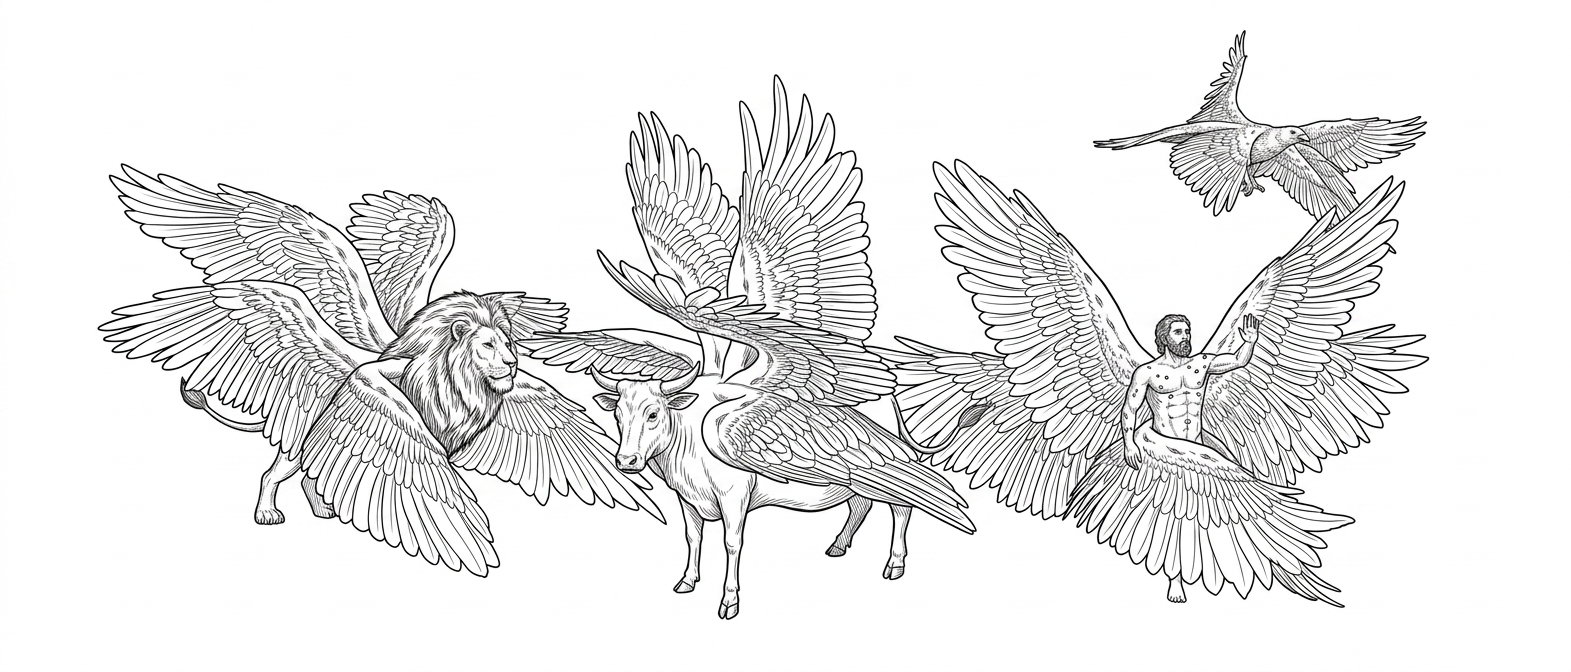
\includegraphics[
    width=1\textwidth, 
    trim=100 50 100 30, 
    clip]{images/four_living_creatures.jpg}
\end{figure}

\begin{ReaderQuestion}
表\ref{table:rev3_comp}對照此三處的異象。請圈出它們相似之處。
\end{ReaderQuestion}

這裡四個大有能力的活物，地上已經沒有任何生物如同他們。
四活物全身上下都有眼睛，牠們觀看並守望上帝所創造的一切，象徵上帝全知與無所不察。\footnote{MacArthur, J. (2007). Osborne, G. R. (2002).}
啟示錄 4:7 與以西結書1:10 是對照的。見表\ref{tab:four-living-creatures-zh}。
{
\renewcommand{\arraystretch}{1}
\small
\begin{longtable}{p{2.6cm} p{2.6cm}}
\caption{四活物：啟示錄4:7與以西結書1:10}
\label{tab:four-living-creatures-zh} \\
\hline
啟示錄 4:7 &
以西結書1:10 \\
\hline
像獅子 & 獅子臉 \\
像牛犢 & 牛臉 \\
像人 & 人臉 \\
像飛鷹 & 鷹臉 \\
\hline
\end{longtable}
}

\begin{ReaderQuestion}
四活物晝夜不住地宣告：「聖哉、聖哉、聖哉，主神是昔在、今在、以後永在的全能者。」上帝的聖潔、永恆與全能，對我們今天的敬拜生活有什麼意義？
\end{ReaderQuestion}

\section{頌讚創造萬有的主}

\begin{ScriptureBox2}{劃出二十四位長老所做的三件事，並圈出他們說上帝配得的原因。}

\item[4:10] 那二十四位長老、就俯伏在坐寶座的面前、敬拜那活到永永遠遠的、又把他們的冠冕放在寶座前、說、

\item[4:11] 我們的主、我們的　神、你是配得榮耀尊貴權柄的．因為你創造了萬物、並且萬物是因你的旨意被創造而有的。

\end{ScriptureBox2}

舊約聖經中，尤其是詩篇，有豐富的頌讚是關於神的創造的。我們在讀啟示錄時，更應該將舊約相關的經文放在一起，形成一個更豐富的認識。
這裡4:11的創造主題可以同時使人想到創世記 1 章、詩篇 33 篇、95 篇及 96 篇。\footnote{Bauckham, R. (1993).}
創世記1章說起初神創造天地，並創造人類。 
詩篇 33 篇說耶和華說有就有．命立就立。
詩篇 95:3–7讚美耶和華是大君王；海洋、山嶺與地的深處都屬於祂，因祂創造萬有，百姓當敬拜祂。
詩篇 96:4–5讚美耶和華超越列國的神明，因祂創造諸天，配受列國敬拜。
上帝不僅是創造萬物的主，也是整個受造界的君王。二十四位長老\idx{02}{二十四位長老}將冠冕放在寶座\idx{20}{寶座}前。一切受造者的尊榮與權柄都源於上帝，最終也當歸於祂。

\begin{ReaderQuestion}
創世記 1 章、詩篇 33、95、96 篇，都從不同角度頌讚上帝的創造。當我們真正認識上帝是萬物的創造主，這會如何改變我們看待自己的生命、工作，以及受造世界的態度？
\end{ReaderQuestion}

\section{沒有配展開書卷的}

\begin{ScriptureBox2}{圈出每一個「配」字，並劃出三個找不到任何人的地方。約翰為什麼大哭？}

\item[5:1] 我看見坐寶座的右手中有書卷、裡外都寫著字、用七印封嚴了。

\item[5:2] 我又看見一位大力的天使、大聲宣傳說、有誰配展開那書卷、揭開那七印呢。

\item[5:3] 在天上、地上、地底下、沒有能展開能觀看那書卷的。

\item[5:4] 因為沒有配展開、配觀看那書卷的、我就大哭。

\end{ScriptureBox2}
\begin{figure}[htbp]
    \centering
    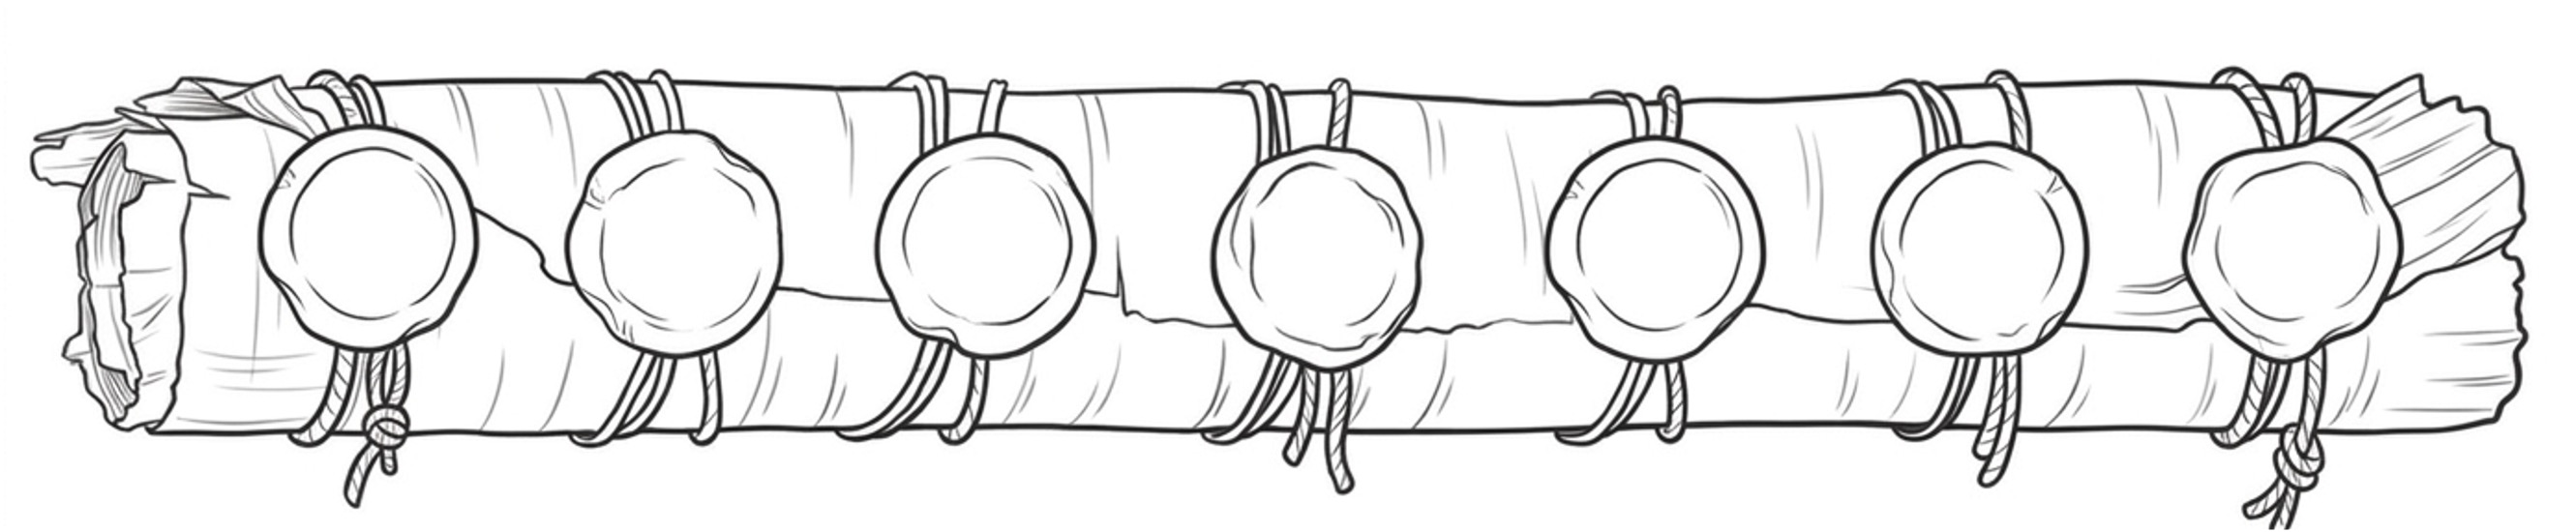
\includegraphics[
    width=1\textwidth, 
    trim=0 0 0 0, 
    clip]{images/scroll_light.jpg}
\end{figure}

歷史掌握在神的手中，並且藉著書卷\idx{10}{書卷}頒給出來。然而，誰配得揭開書卷，使神的旨意進入實現？受造界中竟然無人配得。這使的約翰大哭。
這不僅是因為他無法看見書卷的內容，更是因為若無人配得揭開書卷，上帝的救贖\idx{11}{救贖}與審判\idx{15}{審判}計畫便無法由任何受造者展開。\footnote{這讓我們想到以西結書也有書卷，也都內外寫著字。可是那個書卷是展開的，不是這裡的書卷。以西結書2:9-10：「我觀看、見有一隻手向我伸出來、手中有一書卷。
他將書卷在我面前展開、內外都寫著字、其上所寫的有哀號、歎息、悲痛的話。」}

為什麼是古代的書卷？如果讀者是現代的人或是未來的人，那就不是書卷了。當然，約翰不是在描寫未來的出版科技，而是在使用他所處時代可理解的啟示媒介。
古代以蒲草紙或其他材料製成卷軸。因此，約翰看見的不是一本現代裝訂的書，更不是一份現代的數位文件。


\section{被殺的羔羊才是真正的得勝君王}

\begin{ScriptureBox2}

\item[5:5] 長老中有一位對我說、不要哭．看哪、猶大支派中的獅子、大衛的根、他已得勝、能以展開那書卷、揭開那七印。

\item[5:6] 我又看見寶座與四活物並長老之中、有羔羊站立、像是被殺過的、有七角七眼、就是　神的七靈、奉差遣往普天下去的。

\item[5:7] 這羔羊前來、從坐寶座的右手裡拿了書卷。

\end{ScriptureBox2}
這裡又讓我們看見本書第一章所說的耶穌的形象：祂既是曾經受苦、被殺的主，也是從死裡復活、滿有榮耀\idx{14}{榮耀}與權柄的主。

羔羊\idx{10}{羔羊}使我們想到祂的受死、犧牲與救贖\idx{11}{救贖}；猶大的獅子\idx{12}{猶大的獅子}則使我們想到祂的君王身分、權柄與得勝\idx{11}{得勝}。猶大的獅子，竟以被殺羔羊的形象出現。
基督藉著祂的受死與復活，成就救贖，並顯明君王的權柄。

接著，約翰看見羔羊有「七角七眼」。七眼就是上帝的七靈\idx{02}{七靈}，奉差遣往普天下去。
在舊約中，「角」常用來象徵力量、能力與王權。所以這裡說明基督的權柄與聖靈的工作。

\section{羔羊以自己的血買贖萬民}

\begin{ScriptureBox2}{圈出羔羊配得的原因，並劃出祂為祂的子民所做的事。將此與4:11中上帝配得的原因比較。}

\item[5:8] 他既拿了書卷、四活物和二十四位長老、就俯伏在羔羊面前、各拿著琴、和盛滿了香的金爐．這香就是眾聖徒的祈禱。

\item[5:9] 他們唱新歌、說、你配拿書卷、配揭開七印．因為你曾被殺、用自己的血從各族各方、各民各國中買了人來、叫他們歸於　神、

\item[5:10] 又叫他們成為國民、作祭司、歸於　神．在地上執掌王權。

\end{ScriptureBox2}

羔羊\idx{10}{羔羊}藉著自己的血買贖萬民，使他們歸於上帝。
這救贖\idx{11}{救贖}的歌是蒙恩的罪人能唱的。他們的歌聲中，唱出神對人奇異的恩典\idx{10}{恩典}，唱出人生命的改變，最後在神的榮耀\idx{14}{榮耀}裡。
祂不僅赦免我們的罪，更賜給我們新的身分，使我們成為屬上帝的國度和祭司。從前遠離上帝的人，如今得以親近祂；從前不配敬拜的人，如今竟能與天上的敬拜者一同頌讚羔羊！

\section{從約翰的哭泣到全宇宙的敬拜}

\begin{ScriptureBox2}{圈出每一個參與敬拜的群體。}

\item[5:11] 我又看見、且聽見、寶座與活物並長老的周圍、有許多天使的聲音．他們的數目有千千萬萬．

\item[5:12] 大聲說、曾被殺的羔羊、是配得權柄、豐富、智慧、能力、尊貴、榮耀、頌讚的。

\item[5:13] 我又聽見、在天上、地上、地底下、滄海裡、和天地間一切所有被造之物、都說、但願頌讚、尊貴、榮耀、權勢、都歸給坐寶座的和羔羊、直到永永遠遠。

\item[5:14] 四活物就說、阿們。眾長老也俯伏敬拜。

\end{ScriptureBox2}

%\begin{figure}[htbp]
%    \centering
%    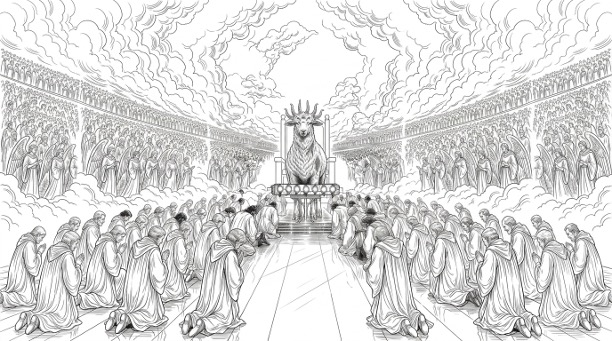
\includegraphics[
%    width=1\textwidth, 
%    trim=0 0 0 0, 
%    clip]{images/lamb_get_scroll2.jpg}
%\end{figure}

這真是偉大的頌讚。敬拜的範圍從千千萬萬的天使，擴展到天上、地上、地底下、滄海裡一切被造之物。萬有都將頌讚、尊貴、榮耀\idx{14}{榮耀}、權勢歸給坐寶座\idx{20}{寶座}的和羔羊\idx{10}{羔羊}，直到永永遠遠。
第四章呈現上帝因創造萬有而配得的敬拜，第五章則呈現羔羊因完成救贖\idx{11}{救贖}而配得的敬拜。
見表\ref{tab:rev4-5-worship-zh} 。

{
\renewcommand{\arraystretch}{1}
\small
\begin{longtable}{p{1cm} p{4cm} p{4cm}}
\caption{啟示錄4--5章的兩首頌讚：創造與救贖}
\label{tab:rev4-5-worship-zh} \\
\hline
敬拜 &
第四章：創造的頌讚 &
第五章：救贖的頌讚 \\
\hline
對象 &
坐寶座的主 &
坐寶座的主與羔羊\\

原因 &
上帝創造了萬物 &
羔羊曾被殺，以自己的血買贖萬民 \\

內容 &
榮耀、尊貴、權柄、創造萬有 &
權柄、豐富、智慧、能力、尊貴、榮耀、頌讚 \\

群體 &
四活物\idx{05}{四活物}、二十四位長老\idx{02}{二十四位長老} &
四活物、二十四位長老、千千萬萬天使，一切被造之物 \\

信息 &
萬有因上帝的旨意而被創造 &
萬民因羔羊的血蒙救贖，歸於上帝 \\
\hline
\end{longtable}
}

\begin{ReaderQuestion}
在你自己的生命中，你可以為什麼事讚美上帝是創造主？又可以為什麼事感謝羔羊是你的救贖主？
\end{ReaderQuestion}

創造與救贖在此交會：那位曾被殺、如今仍然活著的羔羊，與坐在寶座上的上帝一同接受萬有永遠的敬拜。願我們日日敬拜讚美祂創造的大能，讚美的言詞，如海洋般澎湃。願我們日日稱頌祂救贖的恩典\idx{10}{恩典}，感恩的聲音，如江河般奔流，永不止息。

\chapter{羔羊展開書卷（6:1-7:17）}
羔羊在天上揭印，地上展開審判。
前四印給地上的審判是戰爭、饑荒與死亡。第五印轉向為上帝的道和作見證而殉道的聖徒。第六印揭開之後，天地震動、星辰墜落。羔羊忿怒的大日來到。地上的人驚問：「誰能站得住？」所以啟示錄第七章回答這個問題：唯有蒙羔羊寶血潔淨、屬於神的百姓，才能站在寶座和羔羊面前。因此，七印不僅揭示可畏的審判，也見證神對祂子民的保守，以及羔羊所成就的救恩與永恆盼望。

\section{第一印到第四印：四騎士}

\begin{ScriptureBox2}{圈出每匹馬的顏色，並劃出每位騎馬者被賜予的或所做的事。每匹馬出來以前，是誰揭開每一印？}

\item[6:1] 我看見羔羊揭開七印中第一印的時候、就聽見四活物中的一個活物、聲音如雷、說、你來。

\item[6:2] 我就觀看、見有一匹白馬、騎在馬上的拿著弓．並有冠冕賜給他．他便出來、勝了又要勝。

\item[6:3] 揭開第二印的時候、我聽見第二個活物說、你來。

\item[6:4] 就另有一匹馬出來、是紅的．有權柄給了那騎馬的、可以從地上奪去太平、使人彼此相殺．又有一把大刀賜給他。

\item[6:5] 揭開第三印的時候、我聽見第三個活物說、你來。我就觀看、見有一匹黑馬．騎在馬上的手裡拿著天平。

\item[6:6] 我聽見在四活物中、似乎有聲音說、一錢銀子買一升麥子、一錢銀子買三升大麥．油和酒不可蹧蹋。

\item[6:7] 揭開第四印的時候、我聽見第四個活物說、你來。

\item[6:8] 我就觀看、見有一匹灰色馬．騎在馬上的、名字叫作死．陰府也隨著他．有權柄賜給他們、可以用刀劍、饑荒、瘟疫、〔瘟疫或作死亡〕野獸、殺害地上四分之一的人。
\end{ScriptureBox2}

\begin{figure}[htbp]
    \centering
    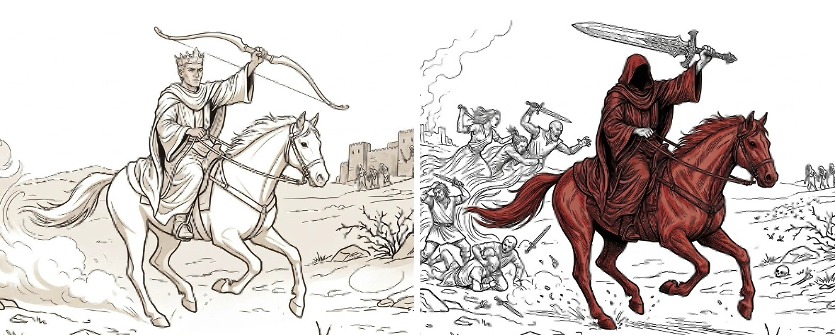
\includegraphics[
    width=1\textwidth, 
    trim=0 0 0 00, 
    clip]{images/horses_white_red.png}
    \caption{第一、二印：白馬勝、紅馬殺}
    \label{fig:horses_white_red.png}
\end{figure}

四匹馬和騎士，帶來地上接連出現的征服、戰爭、饑荒與死亡。
白馬是勝了又勝，紅馬帶來殺戮。
黑馬帶來飢荒使人貧窮，灰馬帶來死亡。
我使用一個口訣，記住它們的特徵。
\begin{center}
\begin{tabular}{ll}
\hline
中文 & English \\
\hline
白馬勝 & White to conquer \\
紅馬殺 & Red to kill \\
黑馬窮 & Black to famine \\
灰馬死 & Pale to die
\end{tabular}
\end{center}


\begin{figure}[htbp]
    \centering
    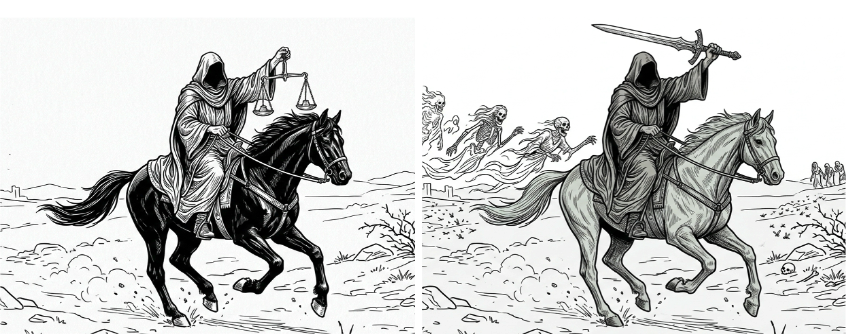
\includegraphics[
    width=1\textwidth, 
    trim=0 0 0 0, 
    clip]{images/horses_black_gray.png}
    \caption{第三、四印：黑馬窮、灰馬死}
    \label{fig:horses_black_gray.png}
\end{figure}

「一錢銀子買一升麥子」形容戰爭之後隨之而來的饑荒，糧食匱乏，物價暴漲。戰爭期間，軍隊往往透過掠奪鄉村取得糧食，甚至以武力奪取食物，使鄉野遭到洗劫。饑荒便成為戰爭帶來的嚴重後果之一。

小麥和大麥是羅馬帝國重要的糧食來源。小麥品質較好，是主要的主食；大麥價格較低，通常是較貧困者食用的穀物。一升小麥大約足夠一個人一天的口糧，而三升大麥則大致相當於一個人一天的口糧。

「一錢銀子」（denarius）通常相當於一個工人一天的工資。因此，一個人辛苦工作一整天，所得幾乎只夠購買自己一天所需的小麥；若買大麥，也只能勉強維持基本的口糧。若還要養活家人，支付住房及其他日常開銷，便更加困難。這正是經文所描繪的饑荒景況：糧食仍然可以買到，卻已昂貴到一般人難以負擔。
至於更稀缺的橄欖油和酒，在糧食匱乏的時候，更是「不可蹧蹋。」

紅、黑、灰馬在經文中寫的相當清楚，那白馬是誰呢？解經家一般有三種解釋。
{
\small
\renewcommand{\arraystretch}{1.1}
\setlength{\tabcolsep}{4pt}
\begin{longtable}{>{\raggedright\arraybackslash}p{2.4cm}|
                  >{\raggedright\arraybackslash}p{7.2cm}}
\caption{白馬騎士的三種解釋}
\label{tab:white-horse} \\
\hline
解釋 & 主要理由 \\
\hline
\endfirsthead

\multicolumn{2}{l}{\small\itshape 表~\thetable（續）} \\
\hline
解釋 & 主要理由 \\
\hline
\endhead

\hline
\endfoot

\hline
\endlastfoot

代表假基督或敵基督勢力

\smallskip
{\color{burgundy}\small\faStar} &
這是許多未來論（Futurist）解經家所持的觀點，見「附錄：各種末世論觀點」。\footnote{MacArthur, J. (2007).}
因為白馬騎士拿著弓，卻沒有提到箭，象徵用欺騙或政治手段征服，並且啟示錄後面出現獸和敵基督的勢力。因此有些解經者認為第一印是末世敵基督活動的開始。馬太福音 24:4-5 先提到假基督迷惑多人，之後才提到戰爭和饑荒，次序與四騎士相近。 \\
\hline
代表軍事征服 &
有些解經者認為白馬不一定是敵基督，因為經文直接提到「勝了又要勝」，所以他們認為是象徵一般性的軍事擴張與帝國征服。征服往往引發戰爭、饑荒和死亡。後面的紅馬、黑馬和灰馬都是有關於戰爭、饑荒和死亡的災難。 \\
\hline
代表基督或福音得勝 &
這是較少數的觀點。支持者認為白色在啟示錄中常象徵聖潔與得勝，因爲啟示錄 19:11 的基督也是騎著白馬。「勝了又要勝」可理解為福音不斷擴展。
可是多數現代解經者不同意此觀點，因為四騎士是一組，應當一起看。而且此處的白馬騎士與啟示錄19章白馬上的基督之間仍存在許多差異。 \\
\end{longtable}
}
\section{第五印：殉道者的呼求}

\begin{ScriptureBox2}{劃出這些人被殺的原因。他們向主求什麼？他們得著什麼，又被告知什麼？}
\item[6:9] 揭開第五印的時候、我看見在祭壇底下、有為　神的道、並為作見證、被殺之人的靈魂．

\item[6:10] 大聲喊著說、聖潔真實的主阿、你不審判住在地上的人給我們伸流血的冤、要等到幾時呢。

\item[6:11] 於是有白衣賜給他們各人．又有話對他們說、還要安息片時、等著一同作僕人的、和他們的弟兄、也像他們被殺、滿足了數目。
\end{ScriptureBox2}

在羅馬人眼中，耶穌的跟隨者是迷信的，為了效忠一位被釘十字架的彌賽亞而犧牲性命，是荒謬可笑的。歷史上的記載也是如此。\footnote{Koester, C. R. (2014).}\footnote{Tacitus, \textit{Ann.} 15.44（塔西佗，《編年史》15.44）；Pliny the Younger, \textit{Ep.} 10.96.8（小普林尼，《書信集》10.96.8）。}\footnote{\textit{Mart. Carp.} 9（《卡爾波殉道記》9）。}

殉道者是「為神的道」並且「作見證」就被殺害。也就是說，他們是專心教導神純全的話語，並做個人見證，這樣子就被殺害，可見是多麼的不公不義。

這段經文對於第一世紀殉道的基督徒，是何等的安慰。祭壇底下的殉道者雖然在地上遭人拒絕，卻蒙上帝悅納。
殉道者的呼求，使我們學到：

\begin{ReaderQuestion}[殉道者給我們的三個功課]
\begin{enumerate}
\item 忠心作見證，即使付上生命的代價（6:9）。
\item 將冤屈帶到聖潔、公義的主面前（6:10）。
\item 在尚未完全成就的公義中，領受上帝的肯定，繼續忍耐等候（6:11）。
\end{enumerate}

\smallskip
這三個功課中，哪一個是你現在最難活出來的？這週你可以怎樣實踐它？
\end{ReaderQuestion}

可是，你可能會問主耶穌不是教導我們要愛仇敵，為逼迫我們的人禱告嗎？那麼，我們該如何理解殉道者的呼求呢？這裡的關鍵在於，我們是否也看見了受害者所承受的不義。

這些殉道者因忠於基督而遭受逼迫，甚至被殺害。他們求上帝伸冤，並不是要親自報復，而是將審判交託給公義的上帝。這段經文說的是一位公義的上帝，也不會忘記那些忠心跟隨祂、為祂作見證的人。
如果殉道者所承認的上帝是「聖潔真實」的，那麼，當惡人殺害無辜者、流無辜人的血時，上帝難道會一直袖手旁觀嗎？
\footnote{Koester, C. R. (2014)}

神的審判有祂所定的時候，甚至要等到殉道者的數目滿足了，才進入祂所定的終局。

神沒有立即執行最後的審判，並不表示祂忽略罪惡或耽延應許，而是因著祂的憐憫與寬容，仍然給人悔改的機會。正如彼得後書 3:9–10 所說：
「主所應許的尚未成就、有人以為他是耽延．其實不是耽延、乃是寬容你們、不願有一人沉淪、乃願人人都悔改。
但主的日子要像賊來到一樣．那日天必大有響聲廢去、有形質的都要被烈火銷化、地和其上的物都要燒盡了。」

\begin{ReaderQuestion}
當我們面對不公義時，可以如何效法第五印的殉道者呢？
\end{ReaderQuestion}

\section{第六印：星辰落地}

\begin{ScriptureBox2}{圈出每一個被震動的受造之物，並劃出每一群躲藏的人。他們在躲避誰的面目？}
\item[6:12] 揭開第六印的時候、我又看見地大震動．日頭變黑像毛布、滿月變紅像血．

\item[6:13] 天上的星辰墜落於地、如同無花果樹被大風搖動、落下未熟的果子一樣。

\item[6:14] 天就挪移、好像書卷被捲起來．山嶺海島都被挪移離開本位。

\item[6:15] 地上的君王、臣宰、將軍、富戶、壯士、和一切為奴的、自主的、都藏在山洞、和巖石穴裡．

\item[6:16] 向山和巖石說、倒在我們身上罷、把我們藏起來、躲避坐寶座者的面目、和羔羊的忿怒．

\item[6:17] 因為他們忿怒的大日到了、誰能站得住呢。
\end{ScriptureBox2}

\begin{figure}[htbp]
    \centering
    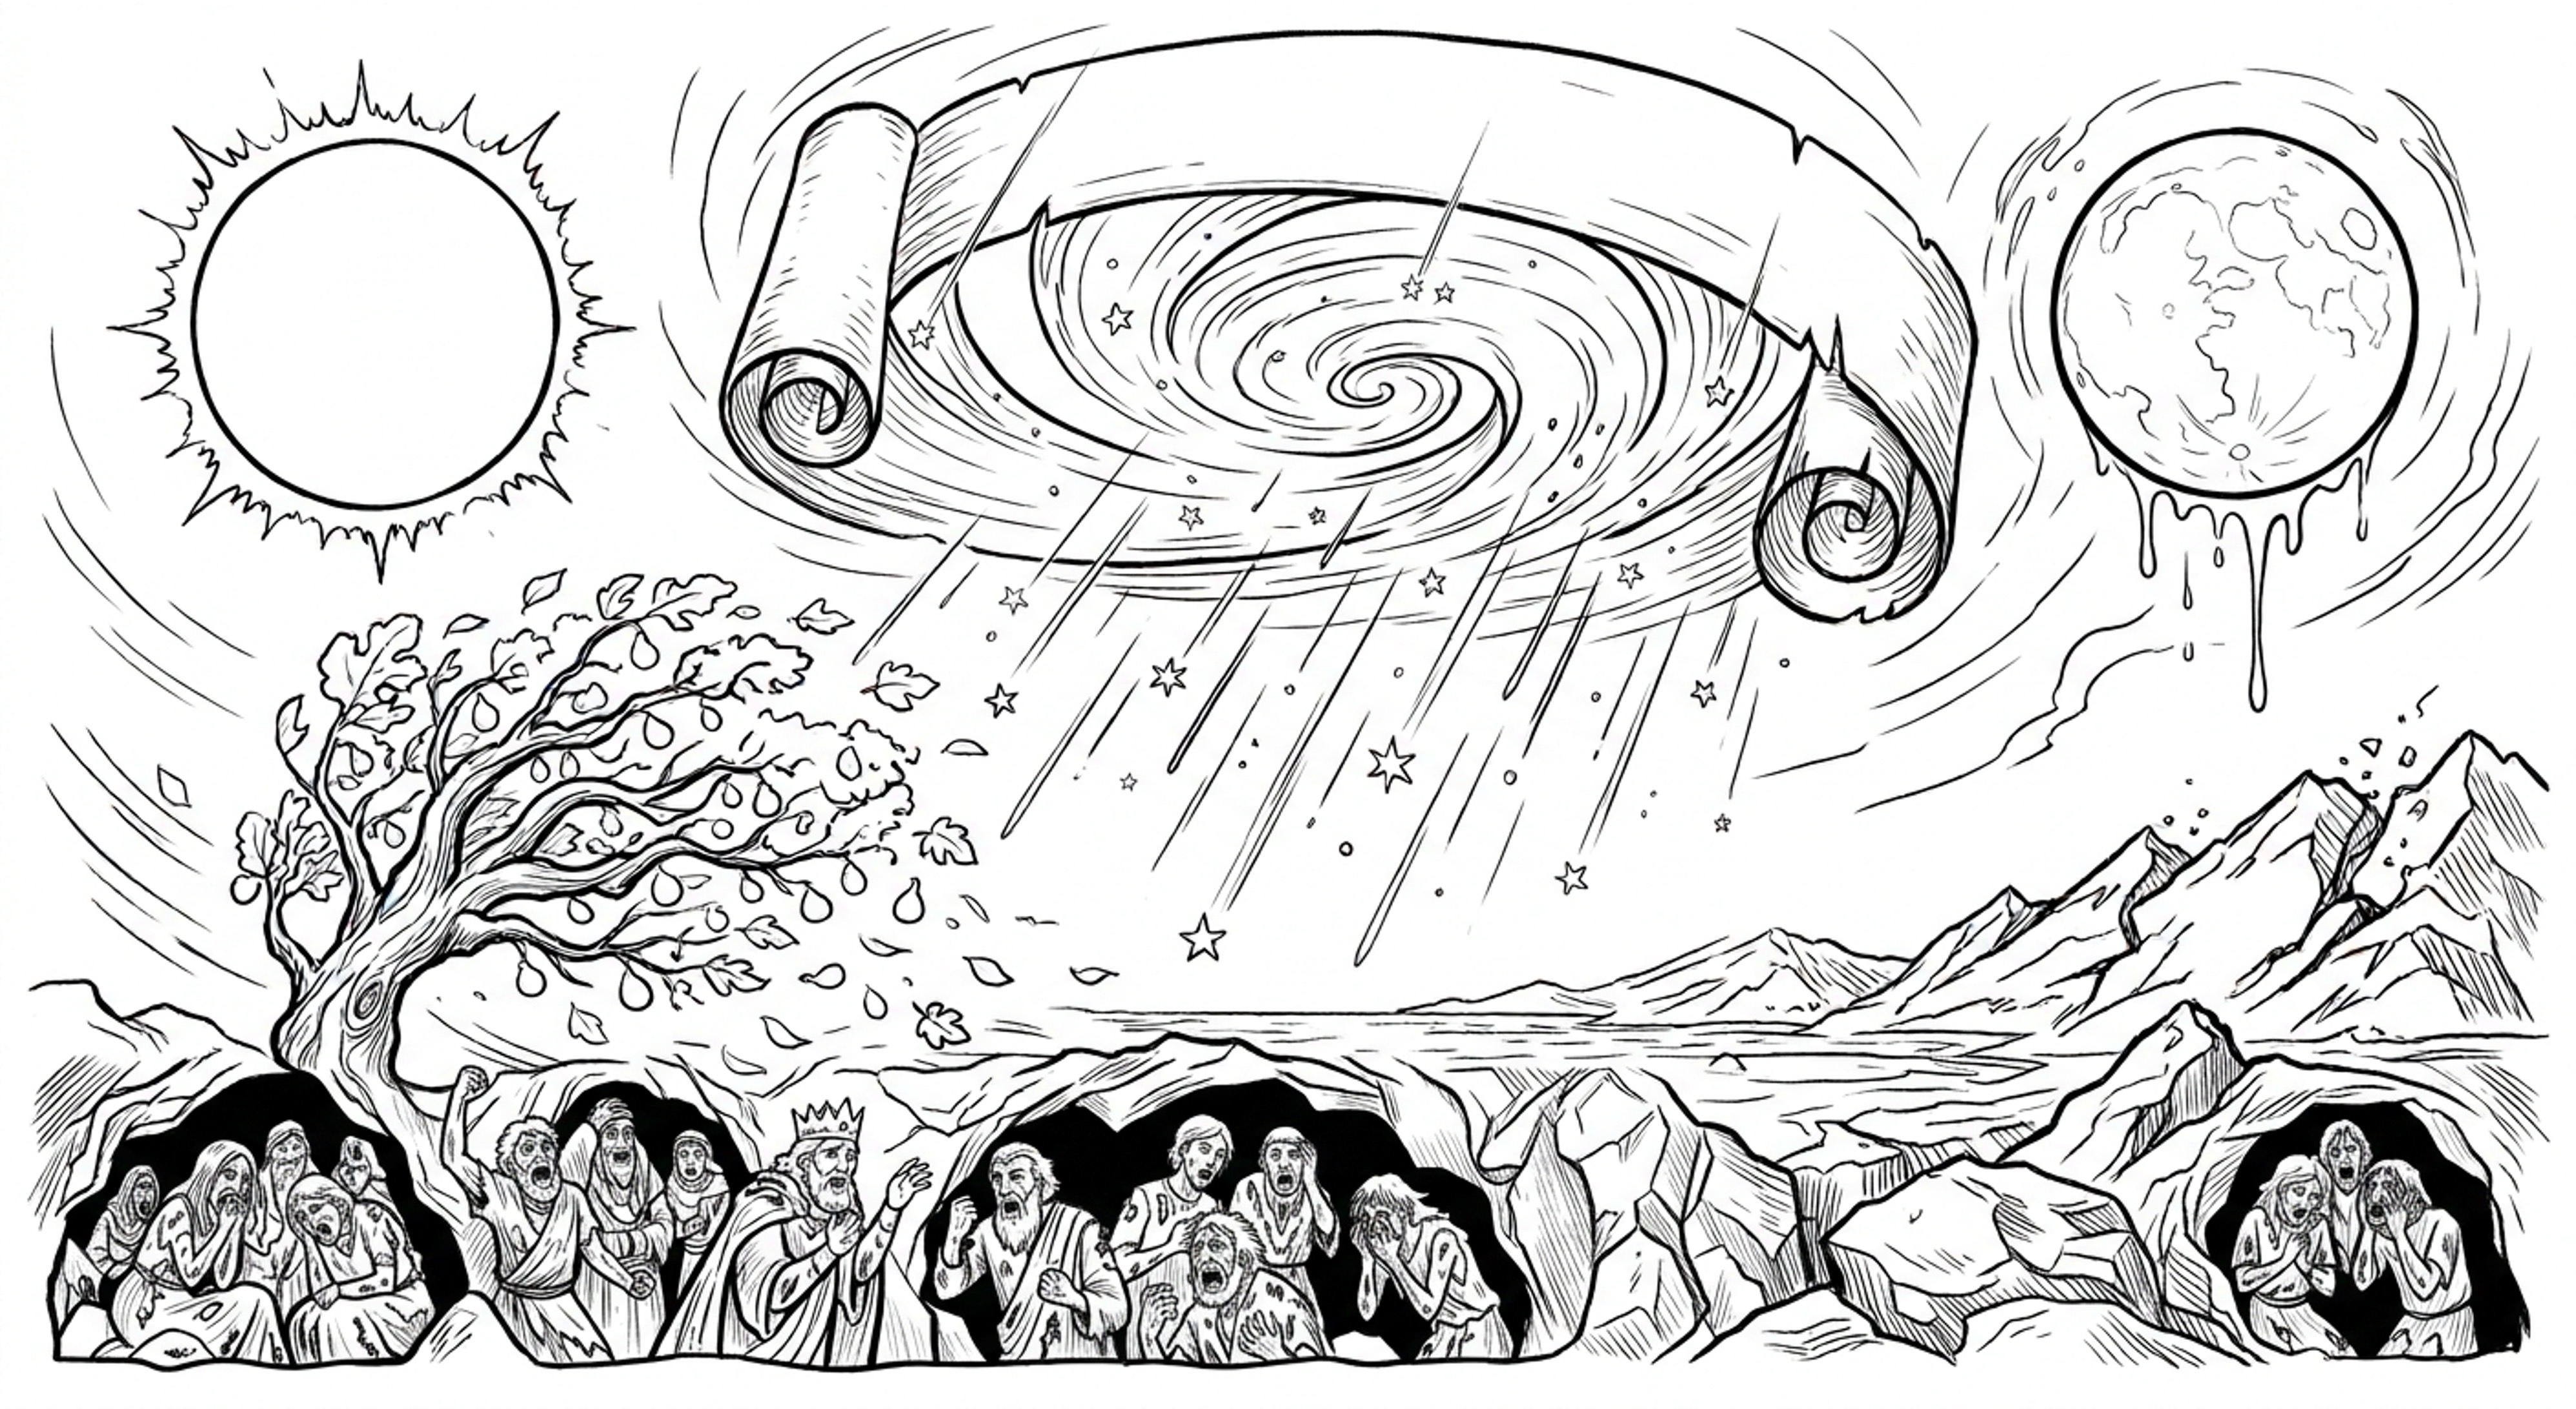
\includegraphics[
    width=1\textwidth, 
    trim=0 0 0 0, 
    clip]{images/seal_6th.jpg}
    \caption{第六印：星辰落地}
    \label{fig:seal_6th}
\end{figure}

我們看到天地震動，地上的人無處可藏，
地上的人恐懼地問，在羔羊公義的憤怒下，誰能站得住？可是到啟示錄第七章我們會看見，那些蒙救贖的人，因為羔羊的血救贖，而得以站立。

{
\small
\renewcommand{\arraystretch}{1}
\begin{center}
\begin{tabular}{ll}
\hline
啟示錄 6:15--17 & 啟示錄 7:9--14 \\
\hline
人躲避上帝和羔羊的面 & 群眾站在上帝和羔羊面前 \\
因忿怒的大日而恐懼 & 穿白衣敬拜上帝 \\
問「誰能站得住？」 & 羔羊的血使蒙救贖人得以站立
\end{tabular}
\end{center}
}

以上的表，可以說是本章主要的信息。
當我們面對羔羊公義的憤怒時，能否坦然站立？
答案不在於我們自己的善行或力量，而在於羔羊已經為我們流血，使我們得蒙救贖、罪得潔淨。

今天，基督仍向我們發出恩典的邀請。
願此書的讀者都接受羔羊的邀請，
不要等到那日才恐懼躲避。
如果你願意的話，現在就悔改、信靠祂的救恩。
因羔羊的恩典，你我都成為那群穿著白衣、站在祂面前，將榮耀和頌讚歸給上帝的人。

\begin{ReaderQuestion}
第六印為什麼使地上的人恐懼？「誰能站得住呢？」這個問題對今天的我們有什麼提醒？
\end{ReaderQuestion}

\subsection*{第一到第六印與馬太福音24章對應}

耶穌在馬太福音24章講的「橄欖山預言」（Olivet Discourse），與啟示錄的第一到第六印，有非常明顯的對應，我列表\ref{tab:seals-matthew24-zh}。

{
\small
\renewcommand{\arraystretch}{1}
\begin{longtable}{p{0.3\textwidth}p{0.4\textwidth}p{0.2\textwidth}}
\caption{啟示錄6章的六印與馬太福音24章的預兆}
\label{tab:seals-matthew24-zh} \\
\hline
\ding{172}-\ding{177}印 & 馬太福音 24 章 & 對應 \\
\hline
\ding{172}白馬，騎馬者出去勝了又要勝 & \textsuperscript{4-5}有人冒基督的名來，迷惑多人 & 假基督、假和平。 \\
\hline
\ding{173}紅馬，奪去太平，使人彼此相殺 & \textsuperscript{6-7}打仗和打仗的風聲，民要攻打民，國要攻打國 & 戰爭、暴力與社會動盪。 \\
\hline
\ding{174}黑馬，天平、糧食昂貴 & \textsuperscript{7}多處必有饑荒 & 糧食短缺及經濟壓力。 \\
\hline
\ding{175}灰馬，死亡及陰間的權柄 & \textsuperscript{7-9}饑荒、地震，並有信徒被交在患難中 & 死亡、災難及苦難。 \\
\hline
\ding{176}殉道者呼求伸冤 & \textsuperscript{9-13}信徒遭患難、被殺、被恨惡，並要忍耐到底 & 信徒受逼迫、殉道及忍耐。 \\
\hline
\ding{177}地震、日月變色、星辰墜落 & \textsuperscript{29-30}日月昏暗、星辰墜落，人子顯在天上 & 同左 \\
\hline
\end{longtable}
}

馬太福音二十四章與啟示錄七印的異象，各有自己的重點。馬太福音強調門徒要謹慎、忍耐到底，並等候人子的來臨。啟示錄進一步以羔羊揭開書卷的異象，表明歷史與審判都在基督的主權之下。

\section{第七印}

\begin{ScriptureBox2}
\item[8:1] 羔羊揭開第七印的時候、天上寂靜約有二刻。
\end{ScriptureBox2}

第七印是在啟示錄8:1，我們放在這裡，與前面六印一起介紹。

第七印沒有像前六印一樣，直接呈現一項災難，而是引出七號的異象（8:2）。七號接續展開上帝的審判，將異象帶入新的階段。

羔羊揭開第七印時，天上寂靜約有二刻。這寂靜如同交響樂中的休止符。眾天使屏息安靜，整個天庭彷彿都在等候，預備迎接接下來大而可畏的審判樂章。這不是審判的終止，而是更猛烈的審判即將展開之前，莊嚴而令人敬畏的停頓。

\subsection*{七印、七號、七碗的順序}

第七印引出七號，第七號吹響時，天上宣告上帝和基督的國度，並提到上帝的忿怒、審判死人及賞賜眾先知和聖徒（11:18）。

但第七號之後沒有立即進入七碗。中間有第12至14章的異象，包括婦人與龍、兩個獸、羔羊與十四萬四千人，以及三位天使的信息。到第15章，約翰看見七位天使拿著末了的七災，並說：「因為　神的大怒在這七災中發盡了。」（15:1）第16章才正式描述七碗倒下。

為了給讀者預覽，我用圖\ref{fig:seals_trumpets_bowls} 解釋七印、七號、七碗的順序。也在下一段順便解釋有關的問題。
\begin{figure}[htbp]
    \centering
    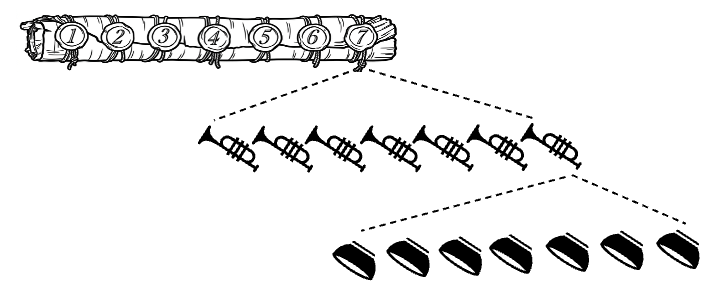
\includegraphics[
    width=1\textwidth, 
    trim=0 0 0 0, 
    clip]{images/seals_trumpets_bowls.png}
    \caption{七印、七號、七碗的順序}
    \label{fig:seals_trumpets_bowls}
\end{figure}

因為七印、七號、七碗有許多審判似乎是類似的場景，就自然的產生了以下的問題。

\begin{InDepth}
\InDepthHeading{七印、七號、七碗是連續發生，還是重述同一個末日審判？}

從字面上來讀，七印、七號、七碗是前後依續發生的。但是會不會是同樣的事件，只是重述，並逐步加深呢？因此，解經者對這三組異象的時間關係，主要有以下兩種理解。

% The table is built row by row, so the box can break between rows.
\par\medskip
{\small\renewcommand{\arraystretch}{1}\setlength{\tabcolsep}{4pt}%
\noindent\begin{minipage}{\linewidth}
\centering
\captionof{table}{七印、七號、七碗的兩種解讀}
\label{tab:seals-trumpets-bowls-zh}
\noindent\rule{\linewidth}{0.4pt}%
\InDepthRow{}{不同審判依序發生}{同樣的審判重述加深}
\InDepthRow{七印}{引出七號。}{敘述上帝的審判。}
\end{minipage}
\InDepthRow{七號}{承接第七印。}{另一角度重述加深審判。}
\InDepthRow{七碗}{承接七號，神的忿怒完全展現。}{再次重述審判。}
\InDepthRow{依據}{第七印引出七號；七號之後出現七碗。}{第六印、第七號、第七碗都出現終局性審判語言。}
\InDepthRow{優點}{重視經文清楚的先後次序。}{能解釋反覆出現的天地震動、上帝忿怒及列國受審判。}
}
\par\medskip

這兩種理解並非在所有方面完全互斥。而採取重述觀點的解經者，也不一定否認經文所呈現的次序。
因此，我們不宜只根據異象的排列，便將每一災精確對應到某個現代歷史事件。
\end{InDepth}

還有，這七印將會如何發生呢？
是在末世大災難期間才會到來，
或是從使徒時代已經開始，一直延伸至基督再來。
或是歷史上反覆出現？
這在神學家有幾個解釋。我特別放在「附錄：各種末世論觀點」。


現在我們繼續讀啟示錄第七章。啟示錄第七章講到有十四萬四千受印，然後有數不清的、各國各族各民各方來的，站在寶座和羔羊面前。

\section{永生神的印保守神的僕人}

\begin{ScriptureBox2}{四位天使執掌著什麼？在地、海和樹木受傷害以前，必須先發生什麼事？}
\item[7:1] 此後我看見四位天使站在地的四角、執掌地上四方的風、叫風不吹在地上、海上、和樹上。

\item[7:2] 我又看見另有一位天使、從日出之地上來、拿著永生　神的印．他就向那得著權柄能傷害地和海的四位天使、大聲喊著說、

\item[7:3] 地與海並樹木、你們不可傷害、等我們印了我們　神眾僕人的額。
\end{ScriptureBox2}

你可能會注意到，在第六印與第七印之間，
怎麼突然插入啟示錄第七章，敘述永生神的印保守神的僕人？

\begin{figure}[htbp]
    \centering
    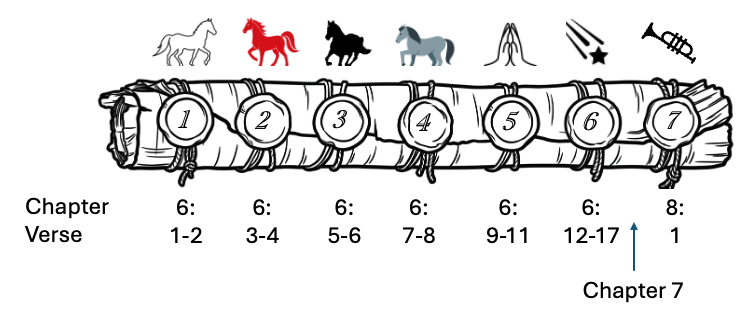
\includegraphics[
    width=1\textwidth,
    trim=0 0 0 0,
    clip]{images/chapter7_insert.png}
    \caption{第六印與第七印之間插入的第七章}
    \label{fig:chapter7_insert}
\end{figure}

這是因為啟示錄6:17以一個尖銳的問題結束：「因為他們忿怒的大日到了，誰能站得住呢？」啟示錄第七章立刻回答這個問題。只有受印的神的僕人以及穿著白衣的數不清的人可以站在寶座和羔羊面前。\footnote{Beale, G. K. (1999).}

「四方的風」是古代舊約常用的語彙，用以表達涵蓋全地的力量。\footnote{但以理書7:2「天的四風颳在大海之上。」耶利米書49:36：「神要使四方的風臨到以攔，將其分散到天下各方。」}因此，此處無須從現代地球幾何或氣象學的角度，質疑「地的四角」與「四方的風」的字面合理性。這裡的重點是神對全地及審判時機的主權。

為什麼先印額，然後施行審判？這是重點。神的印記不是審判的附屬物，而是審判中的身分辨認與救贖安排。我們來看是哪些人受印。

\section{以色列十二支派}

\begin{ScriptureBox2}{數一數支派的數目和每個支派受印的人數。哪一個支派最先被提到？受印的共有多少人？}
\item[7:4] 我聽見以色列人、各支派中受印的數目、有十四萬四千。

\item[7:5] 猶大支派中受印的有一萬二千．流便支派中有一萬二千．迦得支派中有一萬二千．

\item[7:6] 亞設支派中有一萬二千．拿弗他利支派中有一萬二千．瑪拿西支派中有一萬二千．

\item[7:7] 西緬支派中有一萬二千．利未支派中有一萬二千．以薩迦支派中有一萬二千．

\item[7:8] 西布倫支派中有一萬二千．約瑟支派中有一萬二千．便雅憫支派中受印的有一萬二千．
\end{ScriptureBox2}

這裡記載著十四萬四千人受印。他們是誰？這個數字可以是照字面解釋，或也很可能是有象徵的意義。所以一般有三種解釋如表\ref{tab:144000-zh}。

\begin{table}[htbp]
\centering
\renewcommand{\arraystretch}{1}
\caption{十四萬四千人的三種解釋}
\label{tab:144000-zh}
\begin{tabular}{p{2.2cm} p{6.8cm}}
\hline
解釋 & 內容 \\
\hline
以色列 & 指末世從以色列十二支派中受印的十四萬四千人。 \\
象徵教會 & 指由猶太人與外邦信徒組成、屬於神的完整的子民。 \\
象徵以色列 & 以以色列支派象徵末世神的子民，強調神完整地保守祂的子民。 \\
\hline
\end{tabular}
\end{table}





就啟示錄整體而言，十二這個數字反覆出現：十二支派、十二使徒、十二個門、十二個根基，以及新耶路撒冷的十二個城門（啟示錄21:12--14）。
因此，十四萬四千的整齊結構，與啟示錄以十二象徵神子民的完整性，有明顯的呼應。
有些文章試圖直接對應哪一些人才是這十四萬四千人，這裡似乎也不太適合做此對應。
這段經文所強調的重點是神認識屬於祂的子民，並且在審判臨到之際，仍然記念、保守他們。

\section{萬國萬民的敬拜與羔羊的救恩}

\begin{ScriptureBox2}{圈出描述這群人從哪裡來的四個詞，並劃出他們所穿的和手裡所拿的。他們說救恩歸與誰？}
\item[7:9] 此後、我觀看、見有許多的人、沒有人能數過來、是從各國各族各民各方來的、站在寶座和羔羊面前、身穿白衣、手拿棕樹枝．

\item[7:10] 大聲喊著說、願救恩歸與坐在寶座上我們的　神、也歸與羔羊。

\item[7:11] 眾天使都站在寶座和眾長老並四活物的周圍、在寶座前、面伏於地、敬拜　神、

\item[7:12] 說、阿們．頌讚、榮耀、智慧、感謝、尊貴、權柄、大力、都歸與我們的　神、直到永永遠遠。阿們。
\end{ScriptureBox2}

這是多麼壯觀的畫面，那是興奮、有秩序、唱歌的人流。各國各族各民各方的被救贖的人，真正的合一。

\begin{ReaderQuestion}
你得救了嗎？你是不是有確信，將來的你，就會在那個壯闊的人流裡？
如果你還沒有接受基督的救恩，今天就是一個可以認真思想、轉向祂的時刻。耶穌基督為罪人捨命，又從死裡復活；祂邀請你悔改、信靠祂，領受祂白白賜下的恩典。
現在我邀請你接受祂的恩典好嗎？
\end{ReaderQuestion}

我特別寫了以下有關的問題，放在「附錄：常見的問題」：
\begin{itemize}
\item 當你深愛的弟兄（或是姐妹）離世了，可是你走不出傷痛，如何面對？
\item 當復活的時候，人也不娶也不嫁，乃像天上的使者一樣（馬太福音 22:30）
\item 如果將來我在天國，所愛的家人卻不在那裡，我還能快樂嗎？
\end{itemize}

\section{從大患難到永恆安息}

\begin{ScriptureBox2}{劃出這些穿白衣的人是從哪裡來的，以及他們的衣裳是怎樣洗白淨的。然後圈出神和羔羊要為他們所做的一切。}
\item[7:13] 長老中有一位問我說、這些穿白衣的是誰、是從那裡來的。

\item[7:14] 我對他說、我主、你知道．他向我說、這些人是從大患難中出來的、曾用羔羊的血、把衣裳洗白淨了。

\item[7:15] 所以他們在　神寶座前、晝夜在他殿中事奉他．坐寶座的要用帳幕覆庇他們。

\item[7:16] 他們不再飢、不再渴．日頭和炎熱、也必不傷害他們．

\item[7:17] 因為寶座中的羔羊必牧養他們、領他們到生命水的泉源．　神也必擦去他們一切的眼淚。
\end{ScriptureBox2}

血通常使衣裳染紅，可是這裡說，羔羊的血使衣裳洗白淨。在以賽亞書1:18也說到：「你們的罪雖像硃紅、必變成雪白．雖紅如丹顏、必白如羊毛。」

這裡所描繪的得勝，不是信徒憑自己的力量逃離患難，而是羔羊藉著祂的血成就救贖，使神的子民得以進入祂永恆的同在。

\begin{ReaderQuestion}
羔羊的血使衣裳洗白淨，這如何幫助我們理解基督的救恩，並應用在日常生活中？
\end{ReaderQuestion}

從出埃及的拯救，到先知的復興應許，再到羔羊的犧牲與新創造，整個救贖歷史都指向同一個終極盼望：神親自作祂子民的神，羔羊親自作他們的牧者，並擦去他們一切的眼淚。\footnote{
吳榮滁，〈《啟示錄》第12集：額頭蓋印免受傷害〉，台北懷恩堂，2021年9月1日，
https://www.gbc.org.tw/2021/09/20210902/。}

\chapter{基督審判世界（8:1-9:21）}

第七印\idx{02}{七印}揭開之後，天上寂靜約有二刻（8:1）。在這片肅靜之中，約翰看見七位天使領受了七枝號，審判\idx{15}{審判}即將展開。
然後，七號\idx{02}{七號}依次吹響。前四號擊打地、海、江河與天體，第五號和第六號則直接臨到人類。第五、六、七號，又有一隻鷹呼喊為「禍哉、禍哉、禍哉」，顯見審判程度之嚴峻。\footnote{參閱拙著《鷹眼中的榮耀》（\textit{The Eyes of the Eagle: See the Glory}），ISBN 979-8-9907810-9-2，https://drdataman01-ai.github.io/eagle-en-game/。}


不過值得注意的是，這些審判反覆以「三分之一」為限。雖然神的審判是嚴厲的，可是神仍然有節制，留下悔改\idx{10}{悔改}的餘地。只是令人驚訝的是，經歷了這一切之後，人仍舊不悔改（9:20--21）。

\section{禱告如香，升到神面前}

\begin{ScriptureBox2}{天使把什麼和香一同獻上？它升到哪裡？天使接著用香爐做了什麼？}

\item[8:2] 我看見那站在　神面前的七位天使、有七枝號賜給他們。\footnote{啟示錄8:1已於前一章介紹過}

\item[8:3] 另有一位天使拿著金香爐、來站在祭壇旁邊．有許多香賜給他、要和眾聖徒的祈禱一同獻在寶座前的金壇上。

\item[8:4] 那香的煙、和眾聖徒的祈禱、從天使的手中一同升到　神面前。

\item[8:5] 天使拿著香爐、盛滿了壇上的火、倒在地上．隨有雷轟、大聲、閃電、地震。

\item[8:6] 拿著七枝號的七位天使、就預備要吹。

\end{ScriptureBox2}


我們的禱告，上帝認真在聽。禱告如香煙裊裊而上，蒙神悅納。禱告，在舊約中常被用「香煙」形容。詩篇 141:2：「願我的禱告、如香陳列在你面前．願我舉手祈求、如獻晚祭。」在出埃及記 30:1--8和利未記 16:12--13敘述香壇和祭司的禮儀，象徵祈禱。到了啟示錄 8:3--4，地上會幕的金香壇，就象徵天上的敬拜。

\begin{figure}[htbp]
    \centering
    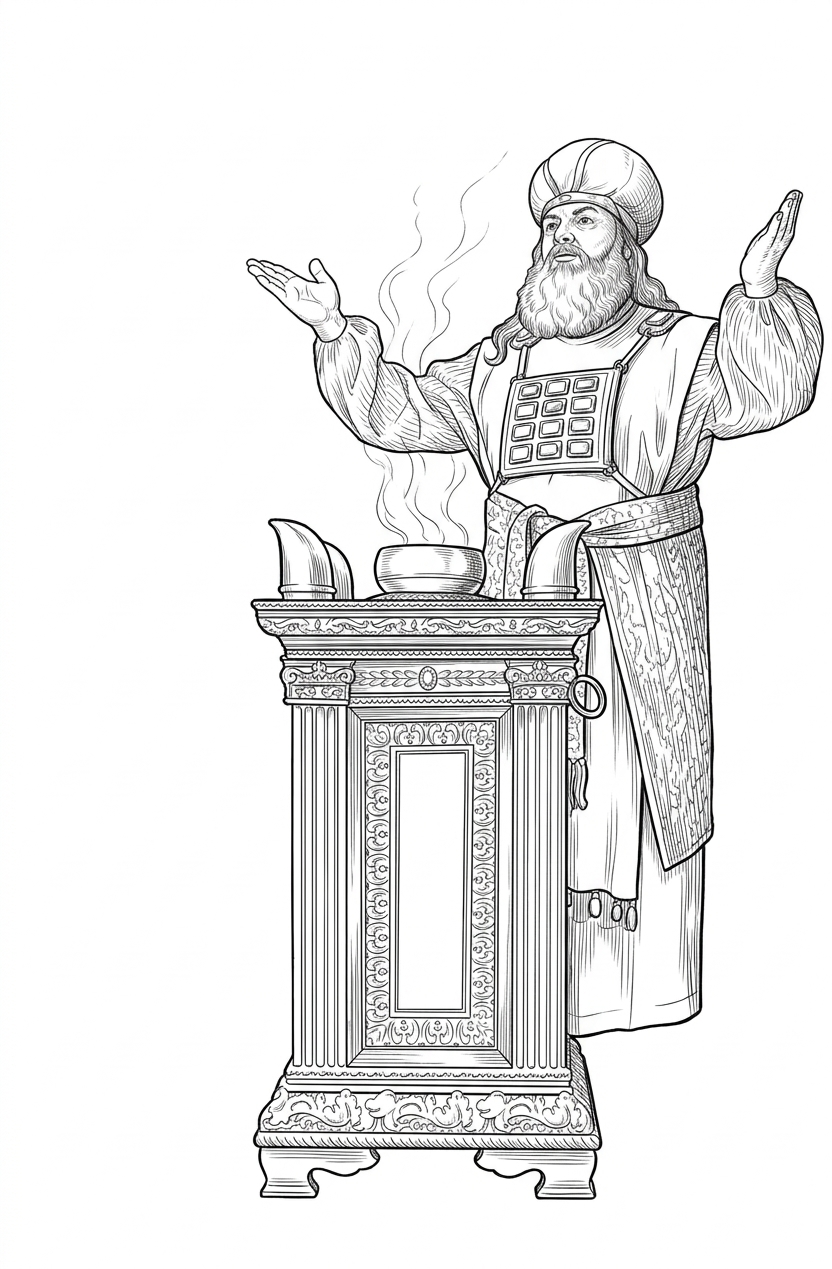
\includegraphics[
    width=0.4\textwidth,
    trim=0 0 0 0,
    clip]{images/golden_altar.jpg}
\end{figure}

\begin{ReaderQuestion}
禱告如香升到神面前（8:3–4）對你而言有什麼意義？當你禱告很久卻看不見改變時，你會如何理解「神聽見了我的禱告」？
\end{ReaderQuestion}

\section{第一號}

\begin{ScriptureBox2}{有什麼丟在地上？圈出地和樹被燒了多少，以及什麼全被燒了。}

\item[8:7] 第一位天使吹號、就有雹子與火攙著血丟在地上．地的三分之一和樹的三分之一被燒了、一切的青草也被燒了。

\end{ScriptureBox2}



\begin{figure}[htbp]
    \centering
    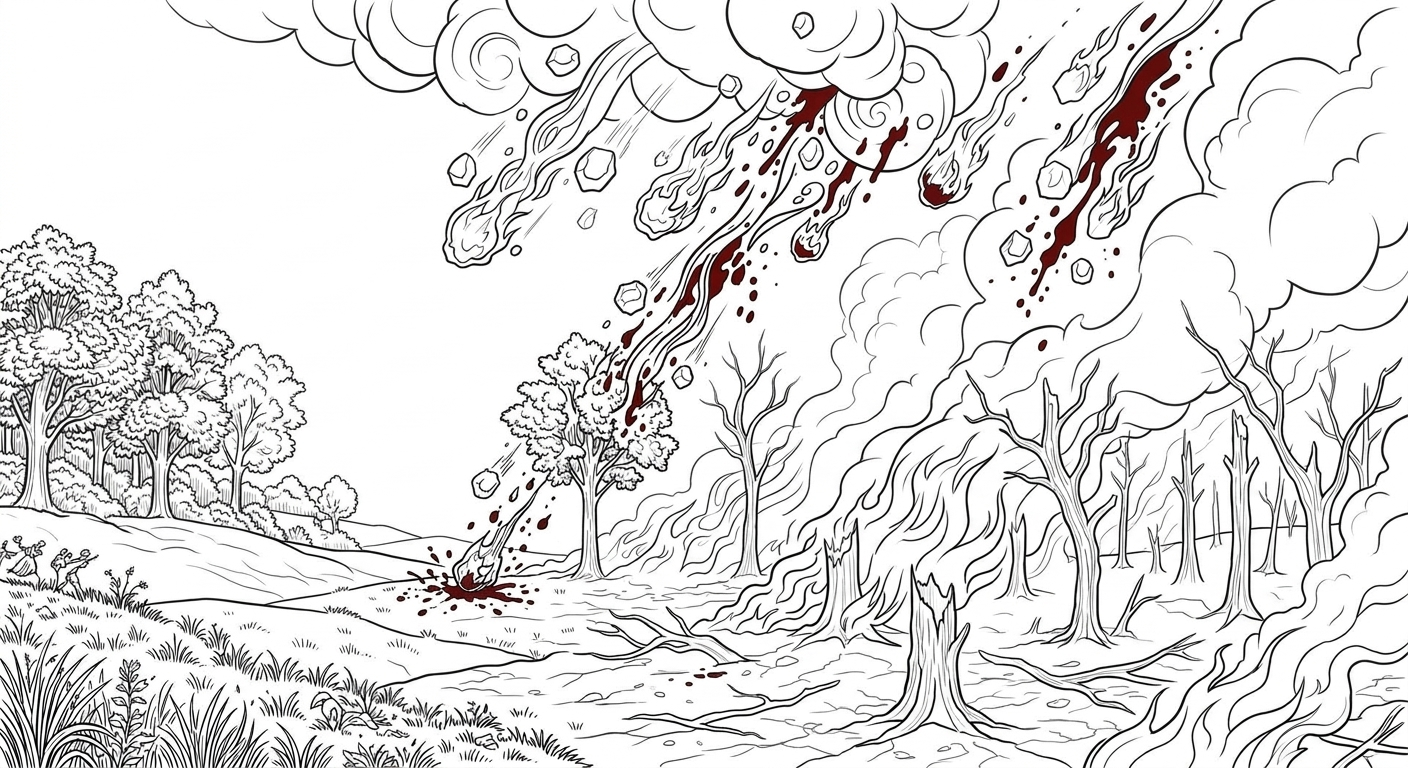
\includegraphics[
    width=1\textwidth, 
    trim=0 0 0 0, 
    clip]{images/trumpet_1st.jpg}
\end{figure}


\section{第二號}

\begin{ScriptureBox2}{數一數8:8–9中「三分之一」出現了幾次。海中有哪三樣受到擊打？}

\item[8:8] 第二位天使吹號、就有彷彿火燒著的大山扔在海中．海的三分之一變成血．

\item[8:9] 海中的活物死了三分之一．船隻也壞了三分之一。

\end{ScriptureBox2}


\begin{figure}[htbp]
    \centering
    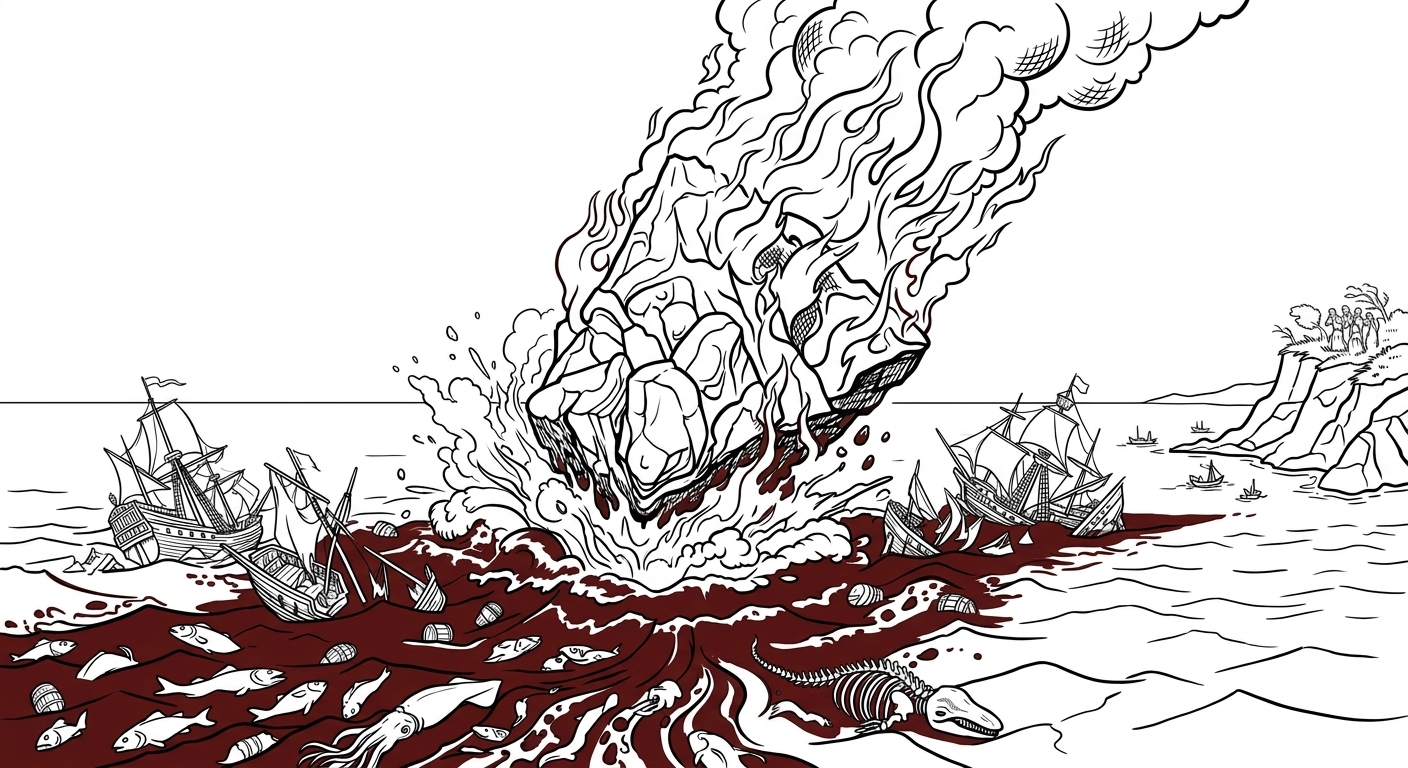
\includegraphics[
    width=1\textwidth, 
    trim=0 0 0 0, 
    clip]{images/trumpet_2nd.jpg}
\end{figure}


\section{第三號}

\begin{ScriptureBox2}{那落下來的星名叫什麼？眾水變成怎樣？喝了那水的人又怎樣？}

\item[8:10] 第三位天使吹號、就有燒著的大星、好像火把從天上落下來、落在江河的三分之一、和眾水的泉源上．

\item[8:11] 這星名叫茵蔯．眾水的三分之一變為茵蔯．因水變苦、就死了許多人。

\end{ScriptureBox2}


\begin{figure}[htbp]
    \centering
    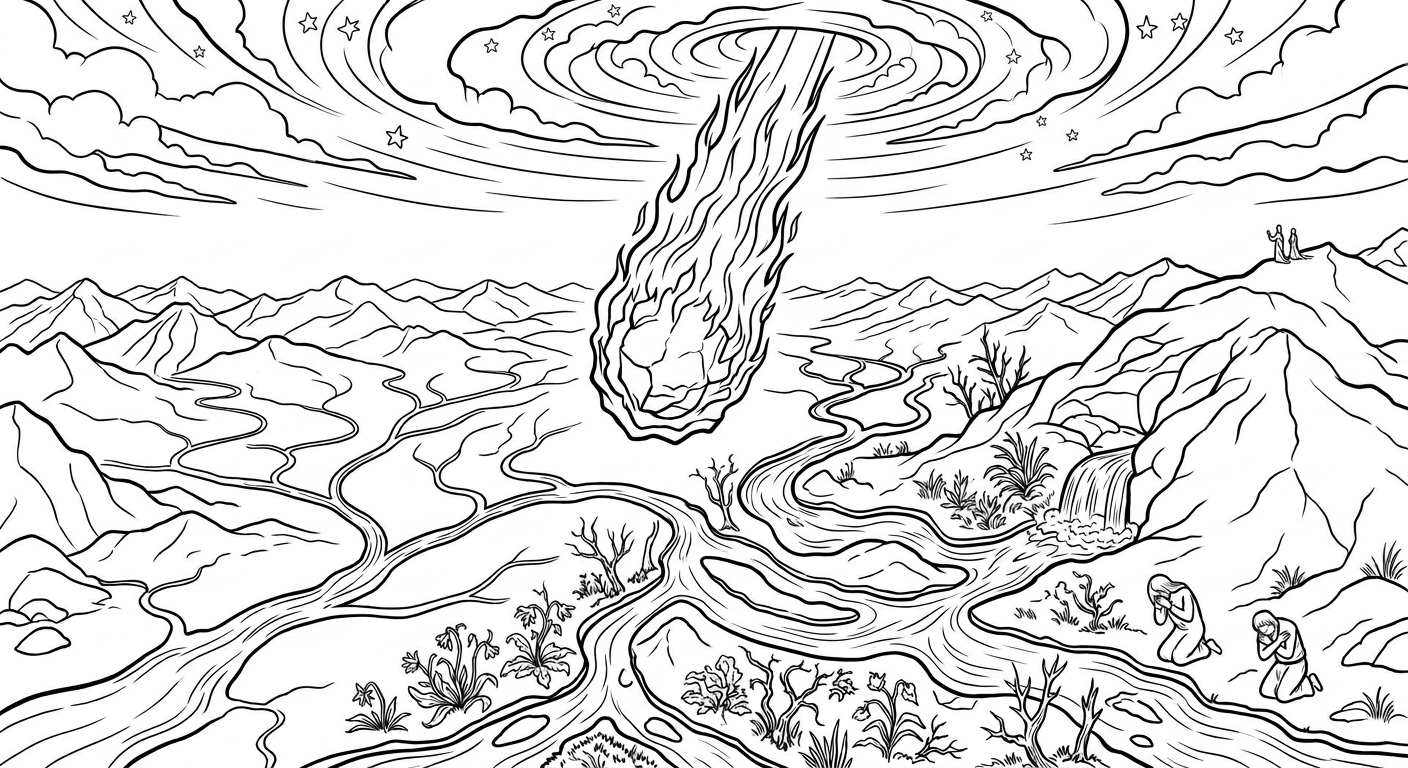
\includegraphics[
    width=1\textwidth, 
    trim=0 0 0 0, 
    clip]{images/trumpet_3rd.jpg}
\end{figure}

「茵蔯\idx{10}{茵蔯}」也叫苦艾、洋艾，希臘文是 apsinthos，英文是wormwood。
這是味道極苦的植物。古代用來驅蟲、入藥，後來也用來製作苦艾酒（absinthe）。
茵蔯在舊約中象徵苦難與審判\idx{15}{審判}。例如耶利米書 9:15說：「我必將茵蔯給這百姓吃，又將苦膽水給他們喝」，以及耶利米哀歌 3:15、阿摩司書 5:7。所以這裡說眾水變為茵蔯，重點在於水變苦、不能喝，帶來死亡。

\section{第四號}

\begin{ScriptureBox2}{天上哪些光體被擊打？各被擊打了多少？白晝和黑夜變成怎樣？}

\item[8:12] 第四位天使吹號、日頭的三分之一、月亮的三分之一、星辰的三分之一、都被擊打．以致日月星的三分之一黑暗了、白晝的三分之一沒有光、黑夜也是這樣。

\end{ScriptureBox2}


\begin{figure}[htbp]
    \centering
    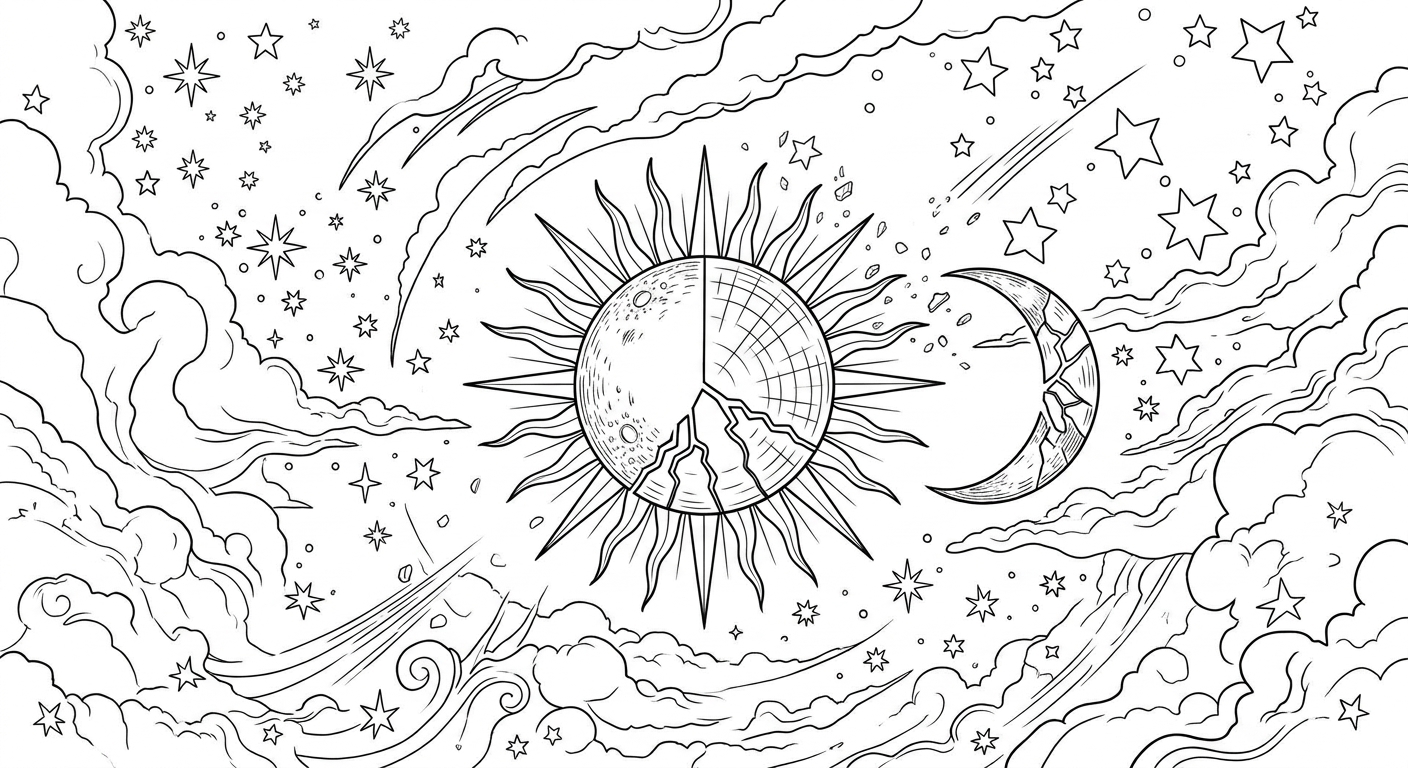
\includegraphics[
    width=1\textwidth, 
    trim=0 0 0 0, 
    clip]{images/trumpet_4th.jpg}
\end{figure}


\section{第五號}

\begin{ScriptureBox2}{在約翰對蝗蟲的描述中，圈出每一個「好像」和「像」。蝗蟲可以傷害誰？牠們又被禁止做什麼？}

\item[8:13] 我又看見一個鷹飛在空中、並聽見他大聲說、三位天使要吹那其餘的號、你們住在地上的民、禍哉、禍哉、禍哉。

\item[9:1] 第五位天使吹號、我就看見一個星從天落到地上．有無底坑的鑰匙賜給他。

\item[9:2] 他開了無底坑、便有煙從坑裡往上冒、好像大火爐的煙．日頭和天空、都因這煙昏暗了。

\item[9:3] 有蝗蟲從煙中出來飛到地上．有能力賜給他們、好像地上蠍子的能力一樣。

\item[9:4] 並且吩咐他們說、不可傷害地上的草、和各樣青物、並一切樹木、惟獨要傷害額上沒有　神印記的人。

\item[9:5] 但不許蝗蟲害死他們、只叫他們受痛苦五個月．這痛苦就像蠍子螫人的痛苦一樣。

\item[9:6] 在那些日子、人要求死、決不得死．願意死、死卻遠避他們。

\item[9:7] 蝗蟲的形狀、好像預備出戰的馬一樣、頭上戴的好像金冠冕、臉面好像男人的臉面。

\item[9:8] 頭髮像女人的頭髮、牙齒像獅子的牙齒。

\item[9:9] 胸前有甲、好像鐵甲．他們翅膀的聲音、好像許多車馬奔跑上陣的聲音。

\item[9:10] 有尾巴像蠍子．尾巴上的毒鉤能傷人五個月。

\item[9:11] 有無底坑的使者作他們的王．按著希伯來話、名叫亞巴頓、希利尼話、名叫亞玻倫。

\item[9:12] 第一樣災禍過去了、還有兩樣災禍要來。

\end{ScriptureBox2}


\begin{figure}[htbp]
    \centering
    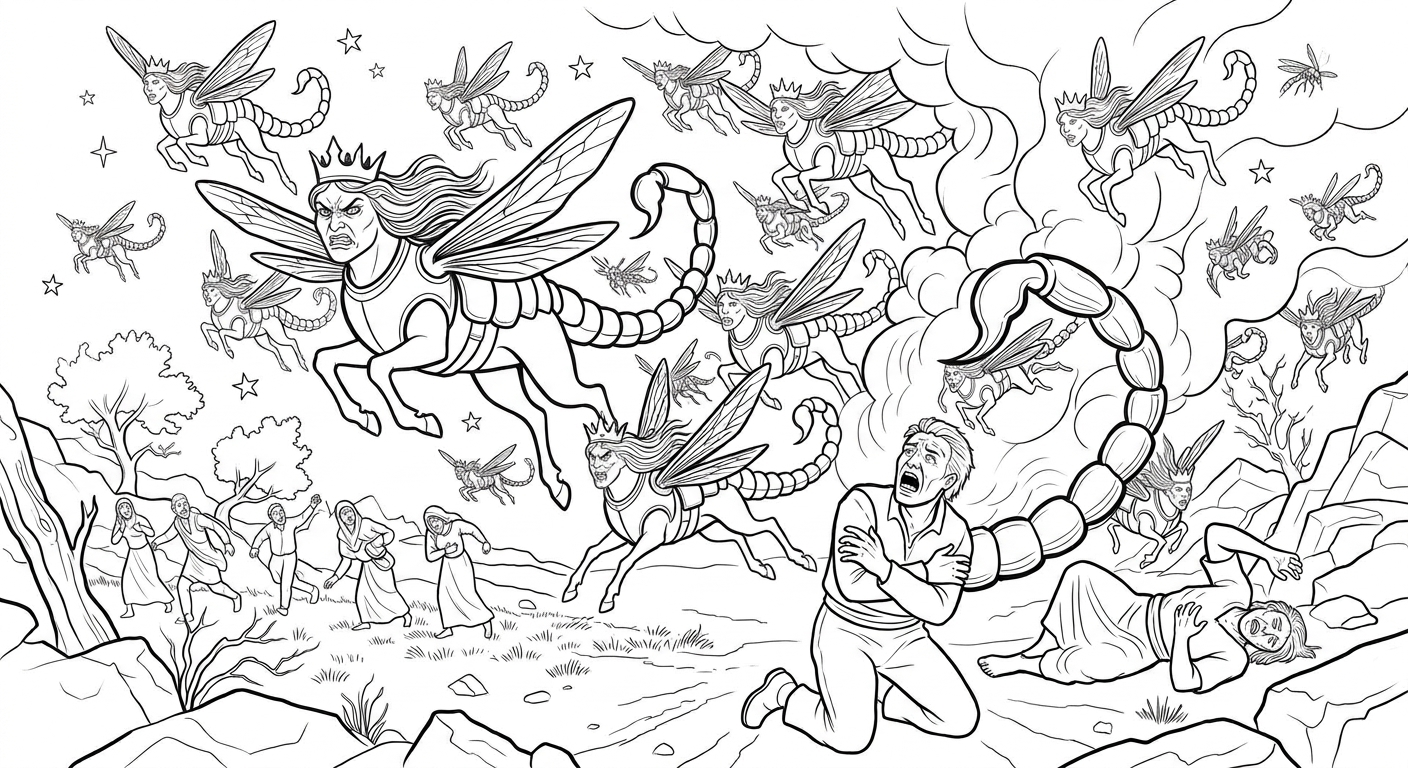
\includegraphics[
    width=1\textwidth, 
    trim=0 0 0 0, 
    clip]{images/trumpet_5th.jpg}
\end{figure}


\section{第六號}

\begin{ScriptureBox2}{9:13的聲音從哪裡出來？將它與8:3比較。然後劃出9:20–21中，那些沒有被殺的人仍然不肯悔改的一切事。}

\item[9:13] 第六位天使吹號、我就聽見有聲音、從　神面前金壇的四角出來、

\item[9:14] 吩咐那吹號的第六位天使、說、把那捆綁在伯拉大河的四個使者釋放了。

\item[9:15] 那四個使者就被釋放．他們原是預備好了、到某年某月某日某時、要殺人的三分之一。

\item[9:16] 馬軍有二萬萬．他們的數目我聽見了。

\item[9:17] 我在異象中看見那些馬和騎馬的、騎馬的胸前有甲如火、與紫瑪瑙、並硫磺．馬的頭好像獅子頭、有火、有煙、有硫磺、從馬的口中出來。

\item[9:18] 口中所出來的火、與煙、並硫磺、這三樣災殺了人的三分之一。

\item[9:19] 這馬的能力、是在口裡、和尾巴上．因這尾巴像蛇、並且有頭用以害人。

\item[9:20] 其餘未曾被這些災所殺的人、仍舊不悔改自己手所作的、還是去拜鬼魔、和那些不能看、不能聽、不能走、金、銀、銅、木、石、的偶像。

\item[9:21] 又不悔改他們那些凶殺、邪術、姦淫、偷竊的事。

\end{ScriptureBox2}


\begin{figure}[htbp]
    \centering
    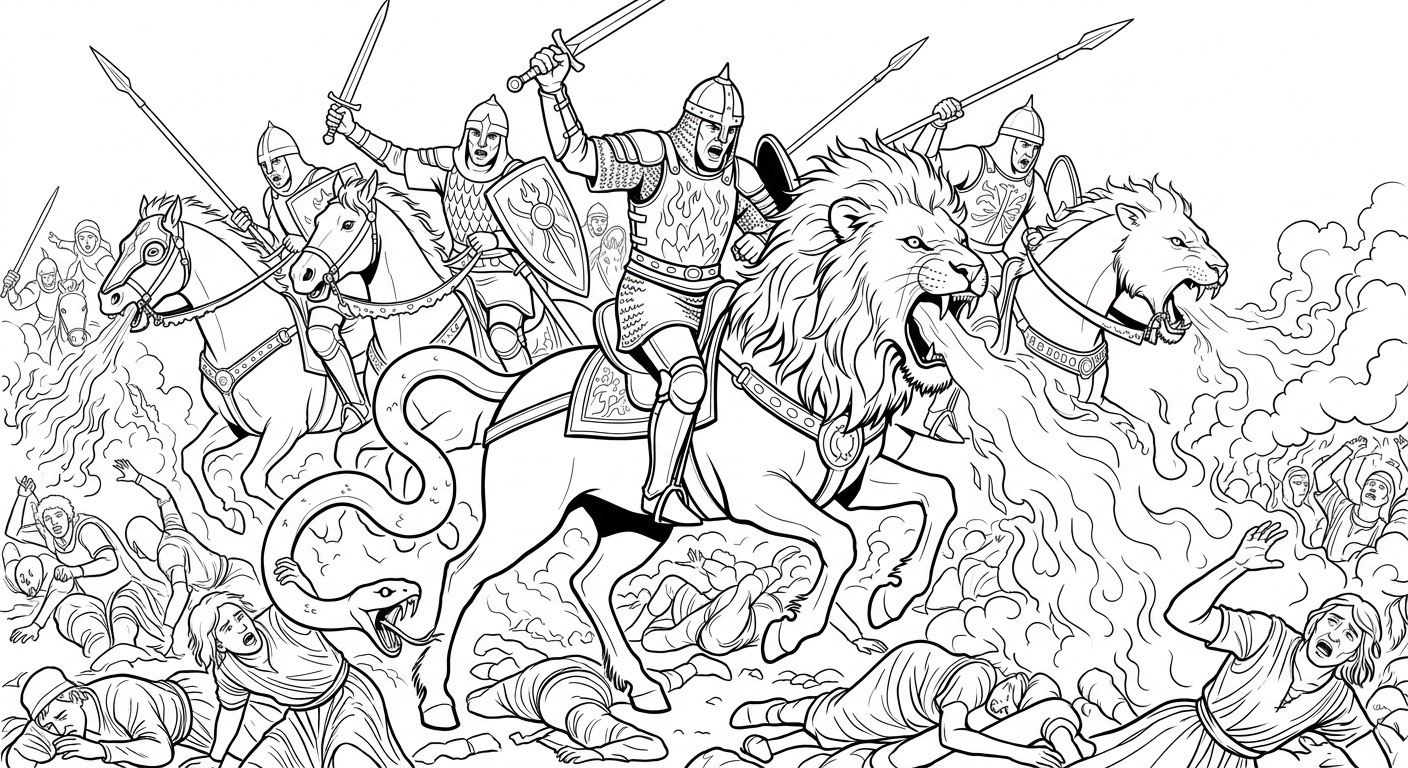
\includegraphics[
    width=1\textwidth, 
    trim=0 0 0 0, 
    clip]{images/trumpet_6th.jpg}
\end{figure}

「那捆綁在伯拉大河\idx{07}{伯拉大河}的四個使者」現在被放出來，執行任務。他們可能是被捆綁的墮落天使或邪靈，或是歷史上的軍事勢力。他們組織了二萬萬的馬軍，是要殺死人類的三分之一。
「馬軍有二萬萬」希臘文直譯是「萬萬的萬萬」，即數量極大的軍隊。所以不一定是 20,000 乘以 20,000 等於 400,000,000。

「伯拉大河」（Euphrates）不僅是以色列\idx{05}{以色列}東北方的重要地理界線，也與神所應許的疆界，以及從東北方而來的外敵和審判\idx{15}{審判}有關。\footnote{例如，神與亞伯拉罕立約時，應許將從埃及河直到伯拉大河一帶的土地賜給他的後裔（創世記 15:18）。另一方面，以賽亞書以伯拉大河水勢洶湧、氾濫溢出的景象，比喻亞述王及其軍隊的勢力，並描寫這股勢力如洪水般臨到猶大（以賽亞書 8:7–8）。} 在這裡，這場審判的範圍已超越古代以色列的疆界，涉及全人類。

這麼大的災禍應該是帶來悔改\idx{10}{悔改}吧？可是災難不能取代悔改。這裡讓我們了解人最大的危機是拒絕悔改。

\begin{ReaderQuestion}
9:20–21特別指出，人經歷災禍之後仍然「不悔改」。為什麼苦難與災難不一定使人悔改？這段經文對我們今天理解「悔改」有什麼提醒？
\end{ReaderQuestion}

值得注意的是，「三分之一」反覆出現。神在七號\idx{02}{七號}中仍然限制。並沒有毀滅整個受造界。


\begin{figure}[htbp]
    \centering
    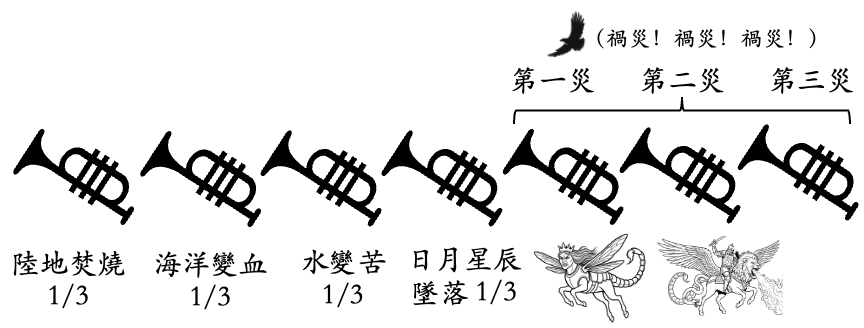
\includegraphics[
    width=1\textwidth, 
    trim=0 0 0 0, 
    clip]{images/trumpets_woes.png}
    \caption{第一號到第七號}
    \label{fig:trumpets_woes}
\end{figure}



\section{未來的事件，古老的語言}

你可能會注意到，神仍讓約翰以馬匹、騎兵和刀劍等第一世紀所熟悉的戰爭武器來描述這些未來事件。可是現在的戰爭已經不使用馬匹和刀劍，而是使用無人機與戰鬥機。以後的戰爭更應該是高度發展的軍事科技。你可能會問，如果啟示錄中的異象確實是未來事件，那麼，為甚麼約翰仍然使用馬匹和刀劍來描述這些異象？神怎麼不直接讓約翰看見並描述未來的軍事科技？甚至可能有人會問，馬是不是坦克？火是不是導彈？蝗蟲\idx{15}{蝗蟲}是不是直升機？

一個比較中肯的答案是，神不是要約翰傳講「未來的武器科技」，而是「神的審判\idx{15}{審判}」。
我們需要了解，看見未來科技未必就是明白神的啟示。神用約翰能傳達的方式給他當時的人以及後來的人。
例如，啟示錄9:7說：「蝗蟲的形狀好像預備出戰的馬。」啟示錄9:17又說「馬的頭好像獅子的頭……」啟示錄9:19則說：「牠們的尾巴好像蛇。」約翰不是說「我看見了馬。」而是不斷使用「好像」的語言來描述他所看見的異象。試想神真的讓約翰看到一架F-35戰機，約翰會怎樣描述？他可能會說：「我看見一隻巨大的鐵鳥，有兩個翅膀，口中吐火，從天上飛過。」啟世錄中大量使用「好像」、「如同」等等，顯示約翰是以他的時代的語言描述所看見的異象。因此，我們如果把啟示錄的敘述直接轉換成阿帕契（Apache）直升機、現代坦克等，並不是好的解經方法。\footnote{Beale, G. K. (1999). Bauckham, R. (1993).}

我們再舉一個例子。例如啟示錄9章的「蝗蟲像戰馬」幾乎明顯對應約珥書中預言關於末世的審判的場景「牠們的形狀如馬，奔跑如馬兵。」（約珥書2:4）
收到約翰書信的讀者就會聯想到約珥書的「 耶和華的日子」「審判 」「末世」。因此神若讓約翰看到一架「F-35」，反而可能破壞了其中跟舊約的關係。

\chapter{在苦難中忠心作見證（10:1-11:19）}

上一章我們讀了第一號到第六號，現在該輪到第七號了吧？然而，啟示錄在第七號之前，插入了兩段故事：「約翰再多說預言」和「兩位見證人」，然後才進入第七號。為什麼要插入這兩個故事呢？這兩段經文都讓我們看見，在神的審判進行之時，祂的子民仍然肩負為祂作見證的使命。即使面對苦難與逼迫，他們仍要忠心見證神的話語，直到基督的國度完全顯明。

\section{約翰再多說預言}

\begin{ScriptureBox}

\item[10:1] 我又看見另有一位大力的天使、從天降下、披著雲彩、頭上有虹．臉面像日頭、兩腳像火柱．

\item[10:2] 他手裡拿著小書卷是展開的．他右腳踏海、左腳踏地．

\item[10:3] 大聲呼喊、好像獅子吼叫、呼喊完了、就有七雷發聲。

\item[10:4] 七雷發聲之後、我正要寫出來、就聽見從天上有聲音說、七雷所說的你要封上、不可寫出來。

\item[10:5] 我所看見的那踏海踏地的天使、向天舉起右手來、

\item[10:6] 指著那創造天和天上之物、地和地上之物、海和海中之物、直活到永永遠遠的、起誓說、不再有時日了．〔或作不再耽延了〕

\item[10:7] 但在第七位天使吹號發聲的時候、　神的奧秘、就成全了、正如　神所傳給他僕人眾先知的佳音。

\item[10:8] 我先前從天上所聽見的那聲音、又吩咐我說、你去把那踏海踏地之天使手中展開的小書卷取過來．

\item[10:9] 我就走到天使那裡、對他說、請你把小書卷給我．他對我說、你拿著喫盡了、便叫你肚子發苦、然而在你口中要甜如蜜。

\item[10:10] 我從天使手中把小書卷接過來、喫盡了．在我口中果然甜如蜜．喫了以後、肚子覺得發苦了。

\item[10:11] 天使〔原文作他們〕對我說、你必指著多民多國多方多王再說預言。

\end{ScriptureBox}

\begin{figure}[htbp]
    \centering
    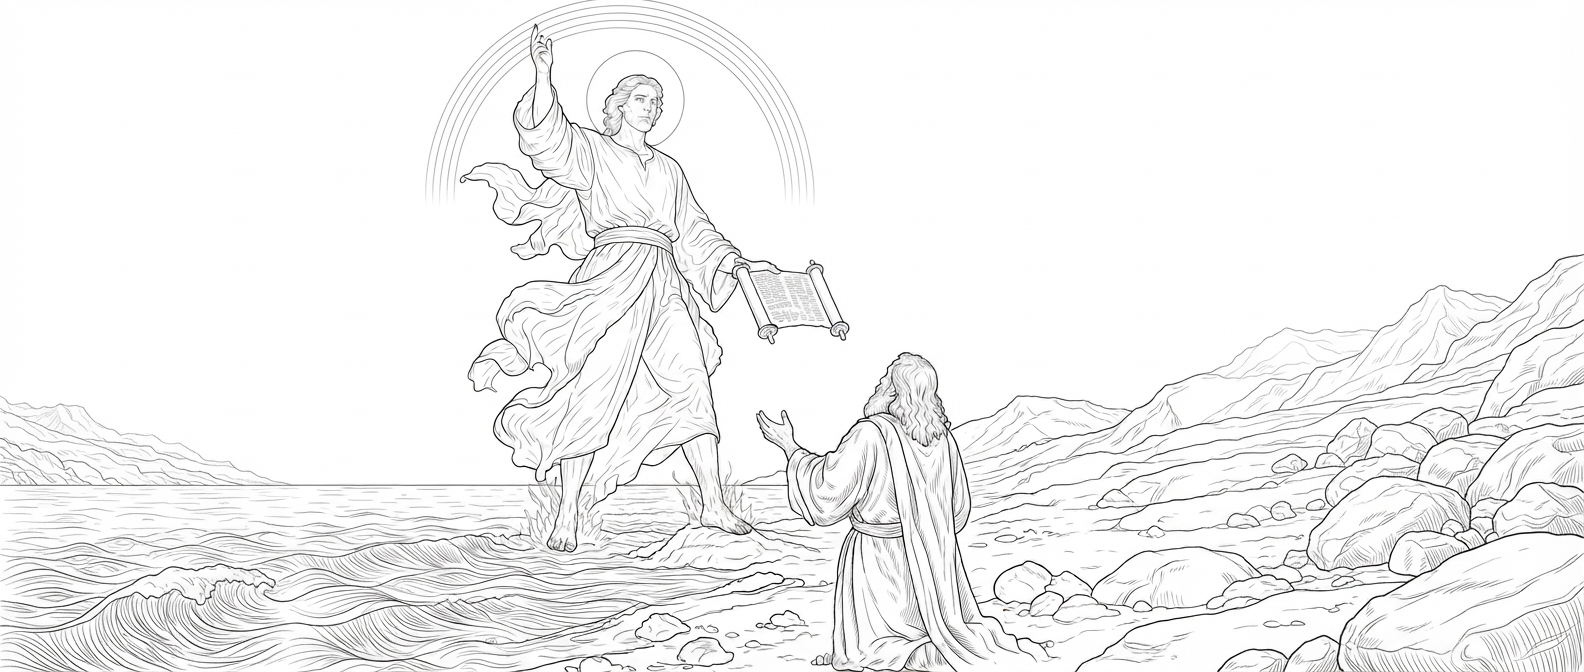
\includegraphics[
    width=1\textwidth, 
    trim=200 0 200 0, 
    clip]{images/small_scroll2.jpg}
\end{figure}

神的話在口中甜如蜜，因為它帶來神的真理並帶來安慰。神的話使得約翰腹中發苦，因為忠心傳揚這真理，也意味著面對審判、苦難與逼迫。

約翰正要寫下所聽見的內容時，卻有聲音從天上吩咐他「不可寫出來。」這表明神決定哪些事情可以讓約翰知道，哪些事情仍然隱藏。
申命記29:29說：「隱祕的事是屬耶和華我們神的；惟有明顯的事是永遠屬我們和我們子孫的。」
我們信仰的重點不在於知道每一個末世細節，而在於相信神掌管歷史，並忠心領受祂已經啟示的真理。
這裡有一個重要的屬靈功課，就是我們要以謙卑的心面對尚未顯明的事，專注遵行神已經向我們啟示的話語。


\section{兩個見證人}

\begin{ScriptureBox}

\item[11:1] 有一根葦子賜給我、當作量度的杖．且有話說、起來、將　神的殿、和祭壇、並在殿中禮拜的人、都量一量。

\item[11:2] 只是殿外的院子、要留下不用量．因為這是給了外邦人的．他們要踐踏聖城四十二個月。

\item[11:3] 我要使我那兩個見證人、穿著毛衣、傳道一千二百六十天。

\item[11:4] 他們就是那兩棵橄欖樹、兩個燈臺、立在世界之主面前的。

\item[11:5] 若有人想要害他們就有火從他們口中出來、燒滅仇敵．凡想要害他們的、都必這樣被殺。

\item[11:6] 這二人有權柄、在他們傳道的日子叫天閉塞不下雨．又有權柄、叫水變為血．並且能隨時隨意用各樣的災殃攻擊世界。

\item[11:7] 他們作完見證的時候、那從無底坑裡上來的獸、必與他們交戰、並且得勝、把他們殺了。

\item[11:8] 他們的屍首就倒在大城裡的街上．這城按著靈意叫所多瑪、又叫埃及、就是他們的主釘十字架之處。

\item[11:9] 從各民各族各方各國中、有人觀看他們的屍首三天半、又不許把屍首放在墳墓裡。

\item[11:10] 住在地上的人、就為他們歡喜快樂、互相餽送禮物．因這兩位先知曾叫住在地上的人受痛苦。

\item[11:11] 過了這三天半、有生氣從　神那裡進入他們裡面、他們就站起來、看見他們的人甚是害怕。

\item[11:12] 兩位先知聽見有大聲音從天上來、對他們說、上到這裡來。他們就駕著雲上了天．他們的仇敵也看見了。

\item[11:13] 正在那時候、地大震動、城就倒塌了十分之一．因地震而死的有七千人．其餘的都恐懼、歸榮耀給天上的　神。

\end{ScriptureBox}

\subsection{量度神的殿和聖城被踐踏}

在聖經的異象中，我們會讀到量度聖殿。例如，以西結書40–48章量度聖殿，撒迦利亞書2:1–5也記載量度耶路撒冷的異象。
那象徵神對祂所量度之物的認定、分別或保守。
殿外的院子不量，因為它被交給外邦人，聖城也要被踐踏四十二個月。神的子民雖然屬於神，卻仍可能在地上遭受逼迫。

多久呢？聖經在不同的異象中，提到幾個彼此呼應的時間：「四十二個月」（啟示錄 11:2）、「一千二百六十天」（啟示錄 11:3），以及「一載、二載、半載」（1+2+$\frac{1}{2}=3\frac{1}{2}$）（啟示錄 12:14）。按照一年十二個月、每月三十天計算，這些時間都相當於三年半。對於這三年半應如何理解，不同的解經觀點有不同的解釋與應用。相關的討論，我放在「附錄：大災難多久？但以理書的七十個七」。無論採取哪一種解經觀點，此三年半都代表一段有限的受苦時期，也就是說敵對神的勢力不是無限期的。


\begin{figure}[htbp]
    \centering
    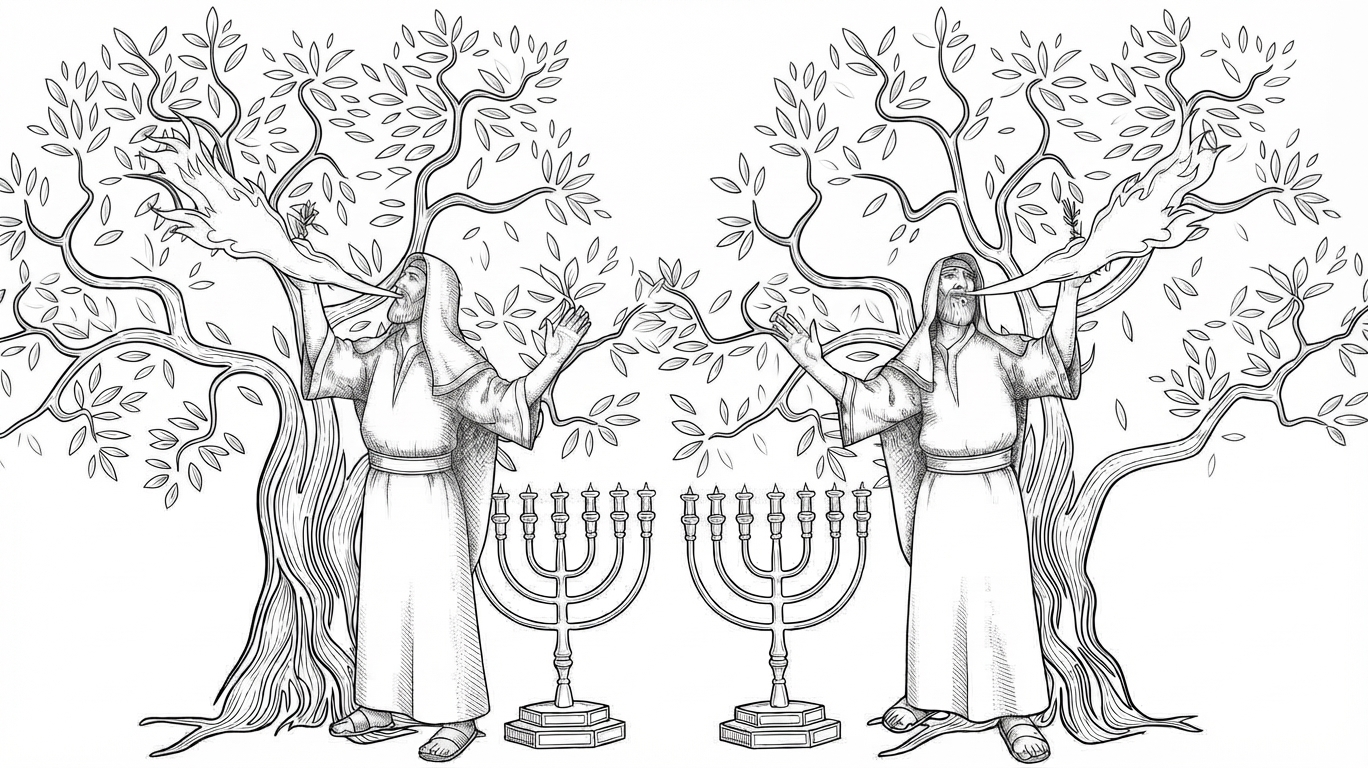
\includegraphics[
    width=1\textwidth, 
    trim=0 0 0 0, 
    clip]{images/two_witnesses.jpg}
\end{figure}


\subsection{兩位見證人是誰？}

此處約翰的預言有大量使用舊約的背景。所以我用表\ref{tab:rev11-ot-background-zh}來了解這些背景以及意涵。


{
\small
\renewcommand{\arraystretch}{1}
%\setlength{\LTpre}{0pt}
%\setlength{\LTpost}{0pt}

\begin{longtable}{
    @{}
    p{0.24\textwidth} |
    p{0.30\textwidth}
    p{0.36\textwidth}
    @{}
}
\caption{啟示錄11章的舊約背景}
\label{tab:rev11-ot-background-zh} \\
\hline 
啟示錄 11 & 舊約背景 & 意涵 \\
\hline
\endfirsthead

啟示錄 11 & 舊約背景 & 意涵 \\
\hline
\endhead

兩個見證人
& 申命記 19:15
& 兩三個見證人的原則 \\

兩棵橄欖樹
& 撒迦利亞 4:1--14
& 橄欖樹、燈臺 \\

兩個燈臺
& 撒迦利亞 4 章；啟示錄 1:20
& 見證與神的子民 \\

火從口中出來
& 耶利米書 5:14
& 神話語審判能力 \\

天閉塞
& 列王紀上 17:1
& 以利亞 \\

水變為血
& 出埃及記7:14-25
& 摩西 \\

各樣災殃
& 出埃及記
& 出埃及記的災禍 \\

無底坑的獸
& 但以理書7章
& 敵對神的政權 \\

所多瑪、埃及
& 創世記、出埃及記
& 敗壞與壓迫神子民的世界 \\

復活
& 以西結書 37 章
& 神使死人得生命 \\

駕雲上天
& 但以理書 7:13；列王紀下 2 章
& 神的榮耀與升天 \\
\hline
\end{longtable}
}

有了以上的舊約背景，我們才能了解不同神學家所提出的，關於兩位見證人是誰的假設。我列表\ref{tab:two-witnesses-zh}如下。

{
\small
\renewcommand{\arraystretch}{1}

\begin{longtable}{
    @{}
    p{0.3\textwidth} |
    p{0.66\textwidth}
    @{}
}
\caption{兩個見證人是誰？}
\label{tab:two-witnesses-zh} \\
\hline 
人物 & 主要依據  \\
\hline
\endfirsthead

兩個見證人是誰？ & 主要依據 \\

\endhead
以諾、以利亞
& 二人都沒有經歷死亡而被神接去 \\

摩西、以利亞
& 火、旱災、降災等神蹟呼應以利亞與摩西；二人一同出現在登山變像。\footnote{Grant R. Osborne、John MacArthur} \\

神將在末世興起的兩位實際人物
& 其具體的傳道、受死、復活與升天。\footnote{John MacArthur 等前千禧年派解經家} \\

忠心的教會和神的子民
& 橄欖樹、燈臺象徵教會。\footnote{G. K. Beale、Craig R. Koester} \\
\hline
\end{longtable}
}

\subsection{第二、三樣災禍包括什麼？}

\begin{ScriptureBox}
\item[11:14] 第二樣災禍過去．第三樣災禍快到了。
\end{ScriptureBox}

第二樣災禍包括第六號所帶來的審判，以及兩位見證人的異象。
第三樣災禍是由第七號吹響開始的。見圖\ref{fig:trumpets_woes}。

\section{第七號響}


\begin{ScriptureBox}

\item[11:15] 第七位天使吹號、天上就有大聲音說、世上的國、成了我主和主基督的國．他要作王、直到永永遠遠。

\item[11:16] 在　神面前、坐在自己位上的二十四位長老、就面伏於地敬拜　神、

\item[11:17] 說、昔在今在的主　神、全能者阿、我們感謝你、因你執掌大權作王了。

\item[11:18] 外邦發怒、你的忿怒也臨到了．審判死人的時候也到了．你的僕人眾先知、和眾聖徒、凡敬畏你名的人連大帶小得賞賜的時候也到了．你敗壞那些敗壞世界之人的時候也就到了。

\item[11:19] 當時　神天上的殿開了．在他殿中現出他的約櫃．隨後有閃電、聲音、雷轟、地震、大雹。

\end{ScriptureBox}

第七號吹響，天上首先宣告的不是另一場災難，而是基督必然掌權的事實。
這裡宣告，神的忿怒已經臨到，審判的時刻已經到了。這不再只是「三分之一」所代表的局部災難，而是神對邪惡施行完全的審判、追討罪惡的時刻。下一章，我們將進一步看見這場爭戰的屬靈本質，以及敵對神的勢力如何走向敗亡。

\section*{小組討論題}

\begin{enumerate}
\item 為什麼神的話會同時「甜如蜜」又「發苦」？
\item 兩個見證人被獸殺害，而且世上的人因他們死亡而歡喜。今天我們是否也會因為害怕人的反應，而不敢忠於基督？
\item 如果神今天要你在自己的家庭、教會、職場或朋友圈中作一個忠心的見證人，你覺得祂可能要你持守什麼、改變什麼，或勇敢說出什麼？
\end{enumerate}


\chapter{龍與獸的權勢，羔羊得勝（12:1–14:20）}

啟示錄第12至13章大量引用或呼應創世記與但以理\idx{07}{但以理}書的異象。若忽略這些舊約背景，我們很容易按照自己的想像解讀，甚至誤解經文的意思。因此，本章將帶領讀者從舊約出發，認識這些異象的背景與象徵，進而理解啟示錄所描繪的屬靈爭戰，以及敵對神的勢力如何與神的救贖\idx{11}{救贖}計畫相抗衡。

那麼，屬神的子民為什麼能勝過魔鬼呢？啟示錄12:11給出了關鍵的一句話：「弟兄勝過他，是因羔羊\idx{10}{羔羊}的血，和自己所見證的道。」基督徒所面對的爭戰，不只是看得見的人事物，也涉及更深的屬靈爭戰。因此，教會的得勝\idx{11}{得勝}不是靠自己的力量擊敗龍，而是因著羔羊的血，並在苦難中仍然持守所見證的道。

接著，第14章描繪天使在天上傳揚永遠的福音\idx{05}{永遠的福音}，呼召地上的人敬畏神，將榮耀\idx{14}{榮耀}歸給祂。為什麽到了這個時候，神還要差派天使給人傳福音？

在這短暫的世上，什麼能存留到永恆？
正是接受神浩大的恩典\idx{10}{恩典}，並且蒙召忠心跟隨基督。基督徒在地上為主作工、為主作見證、培育門徒，都是福分。正如啟示錄14:13所說：「他們息了自己的勞苦，作工的果效也隨著他們。」這提醒我們，為主所作的工不會徒然；即使信徒在世上經歷苦難，仍可以存著盼望，忠心持守到底。

為了幫助讀者掌握這些異象的背景與意義，同時不偏離「羔羊的得勝」這一主題，我整理了以下表格，放在此章的開始，讓讀者先對相關異象、舊約出處及其象徵意義有整體的認識。

{
\small
\renewcommand{\arraystretch}{1}
\setlength{\tabcolsep}{4pt}

\begin{longtable}{
  p{0.21\textwidth}
  p{0.25\textwidth}
  p{0.39\textwidth}
}
\caption{啟示錄12--13章異象的舊約背景}
\label{tab:rev12-13-ot-background-zh} \\
\hline
啟示錄異象 &
舊約背景 &
象徵意義\\
\hline
\endfirsthead

啟示錄異象 &
舊約背景 &
象徵意義 \\
\hline
\endhead

婦人 &
創 37:9-11；賽 54:1-8；66:7-9 &
以色列\idx{05}{以色列}與神的約民 \\

龍 &
創 3:1-15 &
古蛇、撒但\idx{15}{撒但}，以及敵對神的勢力 \\

七頭十角 &
但 7:7-8、24 &
象徵敵對神的帝國權勢 \\

男孩子 &
詩 2:7-9 &
彌賽亞君王耶穌基督 \\

鐵杖 &
詩 2:9 &
彌賽亞統治萬國 \\

一千二百六十天\idx{01}{一千二百六十天}、四十二個月、三年半\idx{03}{三年半} &
但 7:25；12:7 &
一段有限的受苦時期；敵對神的勢力受神限制 \\

天上爭戰 &
但 10:13、20-21；12:1 &
天上屬靈爭戰的背景 \\

海獸\idx{10}{海獸} &
但 7:2-8 &
敵對神及神的子民的帝國權力 \\

十角 &
但 7:7、24 &
君王的政治權勢 \\

地獸\idx{06}{地獸} &
但7章；啟13:11 &
模仿羔羊的外貌，卻傳達龍的權勢，迷惑世人 \\

額上與手上的記號 &
出 13:9、16；申 6:8；11:18 &
神子民將神的話記在手上與額上；
獸的印記\idx{19}{獸的印記}呈現對獸的歸屬與效忠 \\

666 & &
象徵敵對神的權勢及其不完全
\\
\hline
\end{longtable}
}

\begin{ReaderQuestion}
表\ref{tab:rev12-13-ot-background-zh}中幾乎每一個象徵都根源於舊約。將啟示錄與聖經其他部分一同閱讀，如何能保護我們免於揣測或誤解？
\end{ReaderQuestion}

\section{婦人：以色列}

\begin{ScriptureBox2}{圈出婦人和龍各自的樣子。龍等著要做什麼？}

\item[12:1] 天上現出大異象來．有一個婦人、身披日頭、腳踏月亮、頭戴十二星的冠冕．

\item[12:2] 他懷了孕、在生產的艱難中疼痛呼叫。

\item[12:3] 天上又現出異象來．有一條大紅龍、七頭十角、七頭上戴著七個冠冕。

\item[12:4] 他的尾巴拖拉著天上星辰的三分之一、摔在地上．龍就站在那將要生產的婦人面前、等他生產之後、要吞喫他的孩子。

\end{ScriptureBox2}

\begin{figure}[htbp]
    \centering
    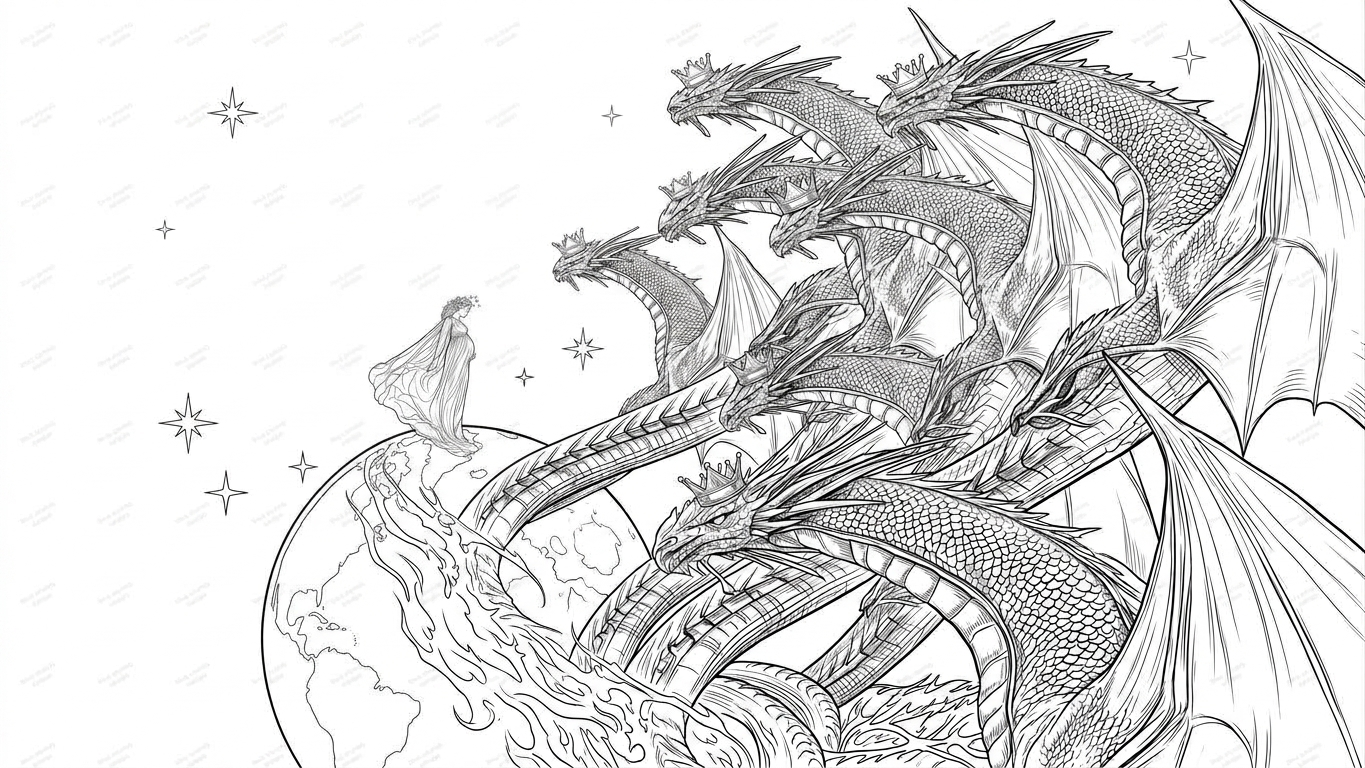
\includegraphics[
    width=1\textwidth, 
    trim=0 0 0 0, 
    clip]{images/woman_and_dragon2.jpg}
\end{figure}

此婦人身披日頭、腳踏月亮、頭戴十二星的冠冕，很容易讓熟悉聖經的讀者想到創世記37:9–11約瑟的夢。夢中出現太陽、月亮和十一顆星，分別代表雅各、拉結與約瑟的十一個哥哥；連同約瑟自己，十二顆星也使人聯想到以色列\idx{05}{以色列}十二支派。
此外，以賽亞\idx{05}{以賽亞}書多次將神的子民或錫安描寫成婦人，描繪神與祂子民的關係（賽 26:17–18；49:14–23；54:1–8；66:7–9）。
尤其是以賽亞66:7-9說「婦人尚未劬勞就生產」，
所以這裡的婦人應當廣義的代表以色列及神的約民。\footnote{G. K. Beale, The Book of Revelation: A Commentary on the Greek Text (Grand Rapids, MI: Eerdmans, 1999), 625.}

當然，由於婦人生下的男孩子是彌賽亞耶穌基督，也有人將婦人理解為耶穌的母親馬利亞。然而，日頭、月亮、頭戴十二星的異象，似乎是廣義的以色列比較妥當。


\section{男孩子：耶穌基督}

\begin{ScriptureBox2}{這男孩子將來要做什麼？他被提到哪裡去了？}

\item[12:5] 婦人生了一個男孩子、是將來要用鐵杖轄管萬國的．〔轄管原文作牧〕他的孩子被提到　神寶座那裡去了。

\end{ScriptureBox2}

這裡直接引用詩篇2:7-9：「你是我的兒子，我今日生你……你必用鐵杖打破他們……」所以男孩子即是彌賽亞君王，是基督。

這裡從男孩子的出生，就接著是龍對男孩子的攻擊，然後就直接說結局「男孩子被提到神寶座\idx{20}{寶座}」，而省略了降生、受死、復活、升天。是把救贖\idx{11}{救贖}歷史事件高度濃縮了。
約翰的焦點不是要講耶穌地上的生平，而是要說龍沒有能力消滅神所立的彌賽亞君王。
\footnote{這正是「預表性／救贖歷史性」的讀法。
預表性：看舊約的人物、事件或制度如何預先指向基督。
救贖歷史性（redemptive-historical）：把經文放在神救贖計畫的整條時間線上來讀，看這段經文在創造、墮落、救贖、成全中位於哪個階段。重點是「進程」。}

\begin{ScriptureBox2}{劃出12:11中弟兄勝過那控告者的三個原因。婦人如何得保護、躲避那龍？龍接著去與誰爭戰？}

\item[12:6] 婦人就逃到曠野、在那裡有　神給他預備的地方、使他被養活一千二百六十天。

\item[12:7] 在天上就有了爭戰．米迦勒同他的使者與龍爭戰．龍也同他的使者去爭戰．

\item[12:8] 並沒有得勝、天上再沒有他們的地方。

\item[12:9] 大龍就是那古蛇、名叫魔鬼、又叫撒但、是迷惑普天下的．他被摔在地上、他的使者也一同被摔下去。

\item[12:10] 我聽見在天上有大聲音說、我　神的救恩、能力、國度、並他基督的權柄、現在都來到了．因為那在我們　神面前晝夜控告我們弟兄的、已經被摔下去了。

\item[12:11] 弟兄勝過他、是因羔羊的血、和自己所見證的道．他們雖至於死、也不愛惜性命。

\item[12:12] 所以諸天和住在其中的、你們都快樂罷．只是地與海有禍了、因為魔鬼知道自己的時候不多、就氣忿忿的下到你們那裡去了。

\item[12:13] 龍見自己被摔在地上、就逼迫那生男孩子的婦人。

\item[12:14] 於是有大鷹的兩個翅膀賜給婦人、叫他能飛到曠野、到自己的地方、躲避那蛇．他在那裡被養活一載二載半載。

\item[12:15] 蛇就在婦人身後、從口中吐出水來像河一樣、要將婦人沖去。

\item[12:16] 地卻幫助婦人、開口吞了從龍口吐出來的水。〔原文作河〕

\item[12:17] 龍向婦人發怒、去與他其餘的兒女爭戰、這兒女就是那守　神誡命、為耶穌作見證的。那時龍就站在海邊的沙上。

\end{ScriptureBox2}


\begin{figure}[htbp]
    \centering
    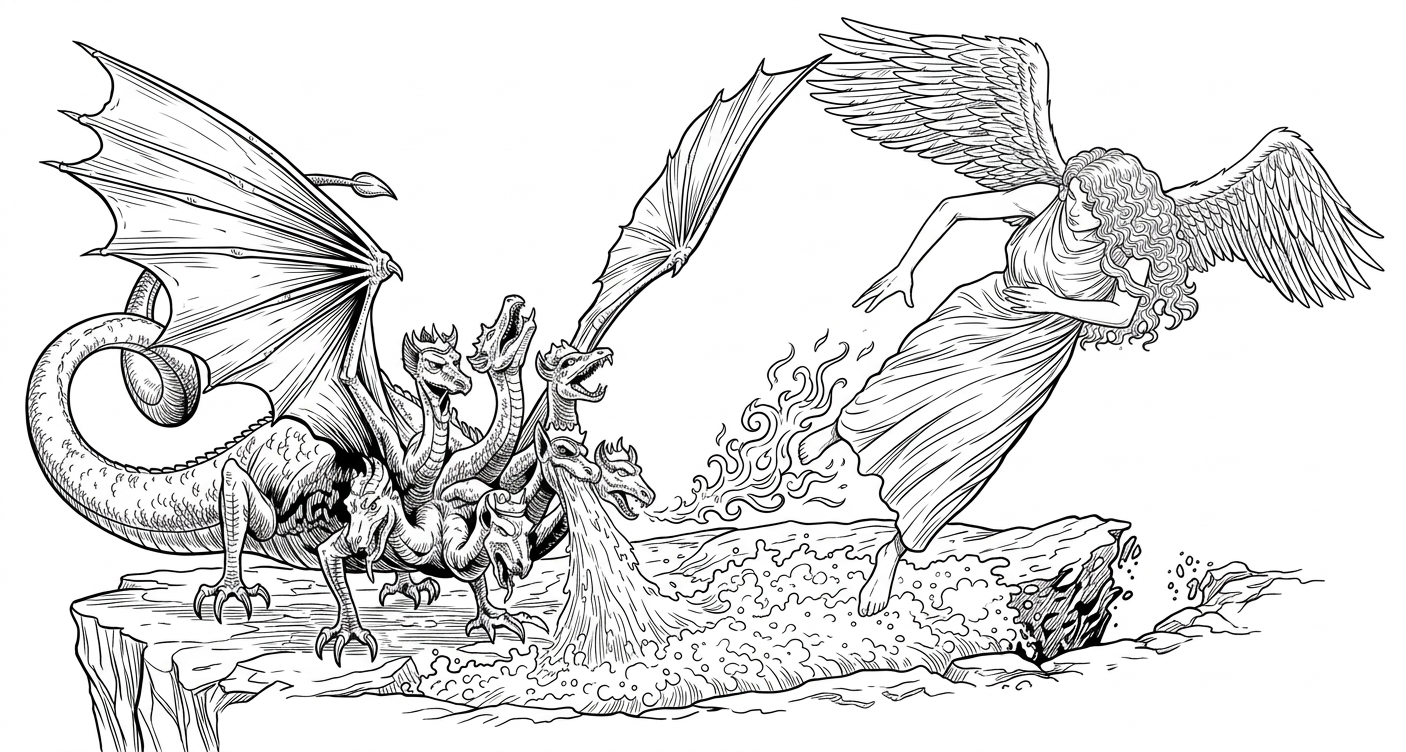
\includegraphics[
    width=1\textwidth, 
    trim=0 0 0 0, 
    clip]{images/woman_fly_away.jpg}
\end{figure}


「一千二百六十天\idx{01}{一千二百六十天}」，是三年半\idx{03}{三年半}（1260/360 = 3.5）。但以理\idx{07}{但以理}書有多處提到三年半。不過如果我們試圖去用某一個世代的三年半來解釋，就常常變得牽強而且失去焦點。最好的解釋就是字面的解釋，是神限制了獸的時間。在此三年半，婦人受神的保護，之後，龍被摔下去，並加緊逼迫\idx{13}{逼迫}婦人和她其餘的兒女。

\begin{ReaderQuestion}
龍的怒氣越來越大，但牠的時候受神限制，婦人也在曠野被養活。當你面對一段似乎越來越艱難、而非逐漸緩和的試煉時期，知道神為它設定了界限，並且一路扶持你，會如何改變你忍耐的方式？
\end{ReaderQuestion}

\section{海獸：地上敵對神的帝國權勢}


\begin{ScriptureBox2}{圈出這獸所像的動物。誰把能力給了這獸？牠可以任意而行多久？}

\item[13:1] 我又看見一個獸從海中上來、有十角七頭、在十角上戴著十個冠冕、七頭上有褻瀆的名號。

\item[13:2] 我所看見的獸、形狀像豹、腳像熊的腳、口像獅子的口．那龍將自己的能力、座位、和大權柄、都給了他。

\item[13:3] 我看見獸的七頭中、有一個似乎受了死傷．那死傷卻醫好了。全地的人、都希奇跟從那獸．

\item[13:4] 又拜那龍、因為他將自己的權柄給了獸．也拜獸說、誰能比這獸、誰能與他交戰呢。

\item[13:5] 又賜給他說誇大褻瀆話的口．又有權柄賜給他、可以任意而行四十二個月。

\item[13:6] 獸就開口向　神說褻瀆的話、褻瀆　神的名、並他的帳幕、以及那些住在天上的。

\item[13:7] 又任憑他與聖徒爭戰、並且得勝．也把權柄賜給他、制伏各族各民各方各國。

\item[13:8] 凡住在地上、名字從創世以來、沒有記在被殺之羔羊生命冊上的人、都要拜他。

\item[13:9] 凡有耳的、就應當聽。

\item[13:10] 擄掠人的必被擄掠．用刀殺人的、必被刀殺。聖徒的忍耐和信心、就是在此。

\end{ScriptureBox2}

「獸」象徵地上的帝國勢力。這是我們從但以理\idx{07}{但以理}書得知的。
但以理書第七章敘述有四個獸從海中上來，但以理書並且解釋那四個獸就是在世上興起的四個王。
接著但以理書第八章以公綿羊與公山羊的異象，預言瑪代波斯與希臘的興起，以及希臘君王的崛起與後續帝國的分裂。\footnote{通常被認為是亞歷山大大帝（但以理書 8:21）。亞歷山大大帝於主前四世紀征服波斯，是約在但以理兩百年之後。}
所以「獸」是指地上的帝國勢力。

這裡的啟示錄，龍被摔下去之後，就站在海邊的沙上。它開始做什麼呢？
它結合海上來的獸與地上來的獸。這裡的海獸\idx{10}{海獸}代表什麼呢？它直接對應但以理書七章。

這裡的「海」代表多國多民。根據啟示錄17:15的解釋，「眾水」就是「多民、多人、多國、多方」。
因此，海獸從「海」中上來，代表從列國中興起、並敵對神和祂子民的地上權勢。
此海獸直接對應但以理書7章的描述。

我製表\ref{tab:rev13-daniel7-zh}來對應此處的異象在兩書中的章節。
{
\renewcommand{\arraystretch}{1}
\small
\begin{longtable}{p{3cm} p{3.5cm} p{2.7cm}}
\caption{啟示錄13章的獸與但以理書7章的四獸}
\label{tab:rev13-daniel7-zh} \\
\hline
啟示錄13 &
但以理書7 &
代表 \\
\hline
1 獸從海中上來 &
2-3 四獸從海上來 &
列國帝國 \\
2 獸有像獅子的口 &
4 第一獸像獅子 &
獅子的意象 \\
2 獸有像熊的腳 &
5 第二獸像熊 &
熊的意象 \\
2 獸的形狀像豹 &
6 第三獸像豹 &
豹的意象 \\
1 可怕權勢 &
7 第四獸極其可怕 &
勝過過去的帝國\\
1 獸有十角 &
7 第四獸有十角 &
帝國性權力 \\
6 獸說褻瀆的話 &
8 小角說誇大的話 &
僭越神的權柄 \\
7 獸與聖徒爭戰 &
21 小角與聖民爭戰 &
逼迫\idx{13}{逼迫}神子民 \\
7 獸「得勝\idx{11}{得勝}」 &
21 小角「勝了他們」 &
暫時性勝利 \\
羔羊\idx{10}{羔羊}最終審判\idx{15}{審判}獸 &
22 「亙古常在者」 &
最終審判 \\
5 四十二個月 &
25 一載、二載、半載 &
逼迫時期有限制 \\
7 任憑獸與聖徒爭戰 &
25 聖民交在獸手中 &
神容許但限制其權勢 \\
獸面對神的審判 &
26-27 獸的權柄最終被除滅 &
獸終必敗亡 \\
\hline
\end{longtable}
}

\begin{ReaderQuestion}
在表\ref{tab:rev13-daniel7-zh}中，啟示錄13章的獸結合了但以理書7章四獸的特徵：獅子、熊、豹和十角。牠甚至「勝過聖徒」，但表格最後卻以牠的權柄被除滅作結。今天世上有哪些權勢在你看來顯得強大或可怕？這個表如何幫助你從神最終審判的角度來看待它們？
\end{ReaderQuestion}

更讓人驚訝的是，龍把權柄給海獸，這海獸受傷又醫好了，結果全地的人都希奇跟從那獸。這裡形成一個很明顯的基督受死又復活的仿冒者。
真正的基督是受死、復活、得榮耀\idx{14}{榮耀}，可是這海獸是似乎死、卻恢復、然後得到普世敬拜。


\begin{figure}[htbp]
    \centering
    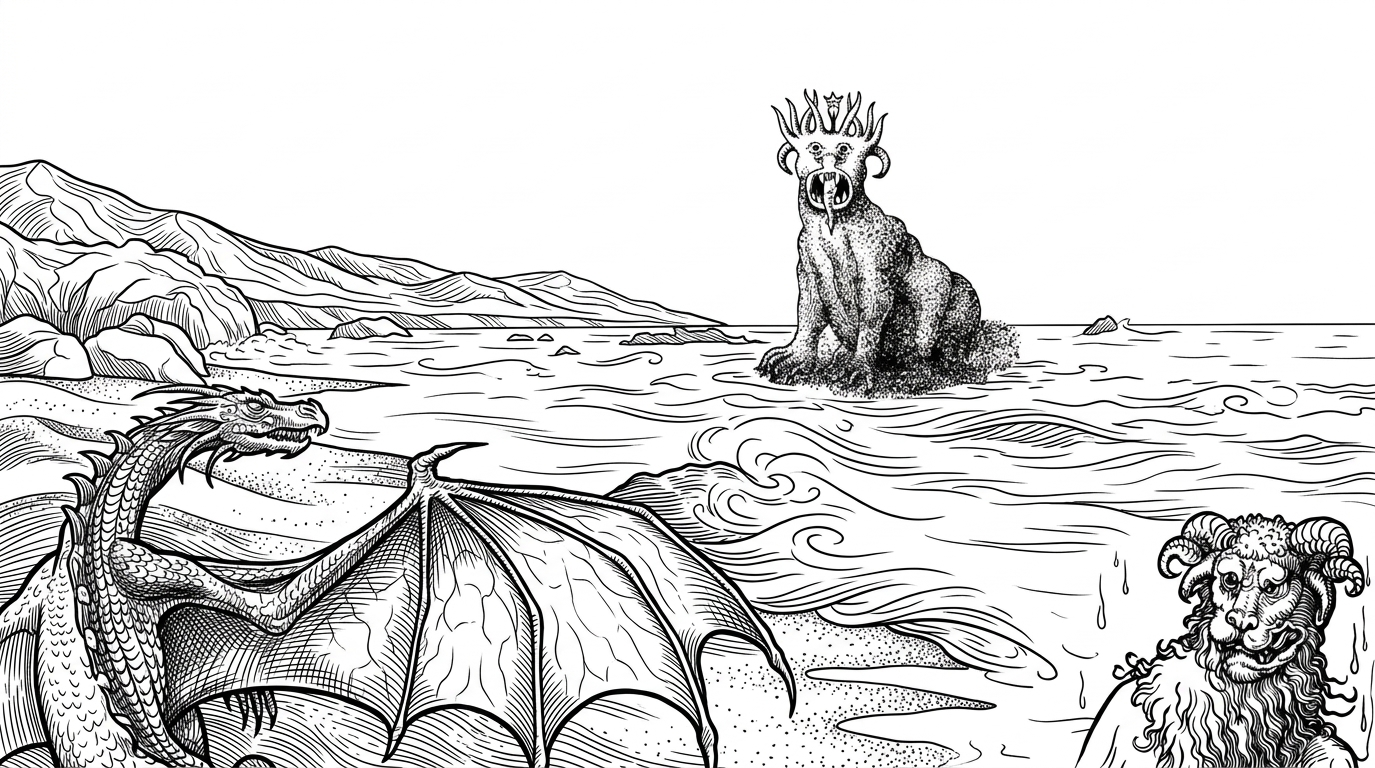
\includegraphics[
    width=1\textwidth, 
    trim=0 0 0 0, 
    clip]{images/dragon_and_breast.jpg}
\end{figure}

\section{從地上來的獸：假先知}

\begin{ScriptureBox2}{第二個獸是什麼樣子？牠說話像什麼？劃出牠叫住在地上的人所做的一切事。}

\item[13:11] 我又看見另有一個獸從地中上來．有兩角如同羊羔、說話好像龍。

\item[13:12] 他在頭一個獸面前、施行頭一個獸所有的權柄．並且叫地和住在地上的人、拜那死傷醫好的頭一個獸。

\item[13:13] 又行大奇事、甚至在人面前、叫火從天降在地上。

\item[13:14] 他因賜給他權柄在獸面前能行奇事、就迷惑住在地上的人、說、要給那受刀傷還活著的獸作個像。

\item[13:15] 又有權柄賜給他叫獸像有生氣、並且能說話、又叫所有不拜獸像的人都被殺害。

\end{ScriptureBox2}

現在我們來看地上的獸。它有像羔羊\idx{10}{羔羊}的外表，但說話像龍。所以這是一個欺騙性的宗教。啟示錄16:13、19:20、20:10後來稱它為假先知\idx{11}{假先知}。

\begin{ReaderQuestion}
地獸外貌像羔羊，說話卻像龍。這提醒我們如何分辨表面敬虔、實際上卻迷惑人的教導？
\end{ReaderQuestion}

因此地獸\idx{06}{地獸}不是單純另一個政治帝國，而是依附在第一獸的統治下行神蹟、欺騙人、推動敬拜獸、使人接受獸的印記\idx{19}{獸的印記}。

所以龍、海獸\idx{10}{海獸}、地獸，形成一個假冒的三位一體\idx{11}{假冒的三位一體}。龍模仿神，獸模仿羔羊，假先知模仿聖靈的工作。

\begin{ReaderQuestion}
龍、海獸與地獸如何彼此配合，形成對神的模仿與敵對？這對我們認識屬靈爭戰有什麼幫助？
\end{ReaderQuestion}

\section{人的數目：666}

\begin{ScriptureBox2}{誰被迫受印記？印記在哪裡？沒有印記的人不能做什麼？}

\item[13:16] 他又叫眾人、無論大小貧富、自主的為奴的、都在右手上、或是在額上、受一個印記。

\item[13:17] 除了那受印記、有了獸名、或有獸名數目的、都不得作買賣。

\item[13:18] 在這裡有智慧。凡有聰明的、可以算計獸的數目．因為這是人的數目、他的數目是六百六十六。

\end{ScriptureBox2}

受了獸的印記\idx{19}{獸的印記}的人，才能夠做買賣。而在此段期間出生的，不接受獸的印記的神的僕人，是不能做買賣的。
因此不接受獸的印記的神的僕人，所受到的逼迫\idx{13}{逼迫}是很大的。他們受到嚴重的經濟排斥，甚至可能必須依靠以物易物的方式維持生活。

但是他們持守真理，只有被殺的羔羊\idx{10}{羔羊}配得敬拜，祂的子民靠著羔羊的血與忠心見證，在獸的逼迫中得勝\idx{11}{得勝}。

為什麼是「666」而不是「777」？這裡比較不適合用666去解釋某種密碼。
我們知道聖經中「7」常與完整、圓滿有關。「666」卻是三重的「不完全」，這裡形成一種強烈的對比：神的完全是「7」，而獸的極度自我高舉是「666」。

有人把獸的印記與當代科技、條碼、晶片、身分證或無現金支付等聯繫起來；這些可以作為現代人的聯想，卻不能直接當作啟示錄對未來科技的預言。經文真正強調的，是對獸的敬拜、效忠，以及由此產生的社會與經濟逼迫。

\begin{ReaderQuestion}
獸的印記與神子民對神的忠心有什麼對比？當信仰與經濟利益或社會壓力發生衝突時，我們應當如何持守信仰？
\end{ReaderQuestion}


\section{羔羊與祂的百姓同在}

龍、海獸\idx{10}{海獸}、地獸\idx{06}{地獸}，形成的假冒的三位一體\idx{11}{假冒的三位一體}的異象令人震撼。
然而，第14章把我們的目光重新帶回羔羊\idx{10}{羔羊}。

約翰看見羔羊站在錫安山，與祂同在的有十四萬四千人\idx{02}{十四萬四千人}。他們額上寫著羔羊和祂父的名，表明他們真正所屬的不是獸，而是神。他們跟隨羔羊，無論祂往哪裡去；他們在患難中仍然持守神的誡命和耶穌的真道。

第13章的假冒的三位一體，與第14章真正的羔羊，成為一個重要的對比。獸要求人敬拜牠，可是我們看見羔羊的百姓敬拜祂。世界可能用權勢、恐懼和利益逼迫\idx{13}{逼迫}人妥協，但神認得屬祂的人。

接著，三位天使宣告審判\idx{15}{審判}已經來到。第一位天使宣告永遠的福音\idx{05}{永遠的福音}，呼召萬民敬畏神、將榮耀\idx{14}{榮耀}歸給祂；第二位宣告巴比倫\idx{04}{巴比倫}傾倒；第三位警告拜獸的人將面對神的審判。最後，兩幅收割\idx{06}{收割}的圖畫把我們帶到歷史的終局：莊稼成熟了，葡萄也熟透了，神的審判必然來到。

然而，在這些嚴肅的審判信息中，神特別賜下一句安慰：

「從今以後，在主裡面而死的人有福了。」

他們雖然在地上經歷勞苦，甚至為基督而死，但他們的勞苦並沒有徒然。他們「息了自己的勞苦」，「作工的果效也隨著他們」。


\begin{ScriptureBox2}{十四萬四千人的額上寫著什麼？劃出14:4–5中描述他們的每一句話。}
\item[14:1] 我又觀看、見羔羊站在錫安山、同他又有十四萬四千人、都有他的名、和他父的名、寫在額上。

\item[14:2] 我聽見從天上有聲音、像眾水的聲音、和大雷的聲音．並且我所聽見的好像彈琴的所彈的琴聲。

\item[14:3] 他們在寶座前、並在四活物和眾長老前唱歌、彷彿是新歌．除了從地上買來的那十四萬四千人以外、沒有人能學這歌。

\item[14:4] 這些人未曾沾染婦女、他們原是童身。羔羊無論往那裡去、他們都跟隨他。他們是從人間買來的、作初熟的果子歸與　神和羔羊。

\item[14:5] 在他們口中察不出謊言來．他們是沒有瑕疵的。

\end{ScriptureBox2}



%\begin{figure}[htbp]
%    \centering
%    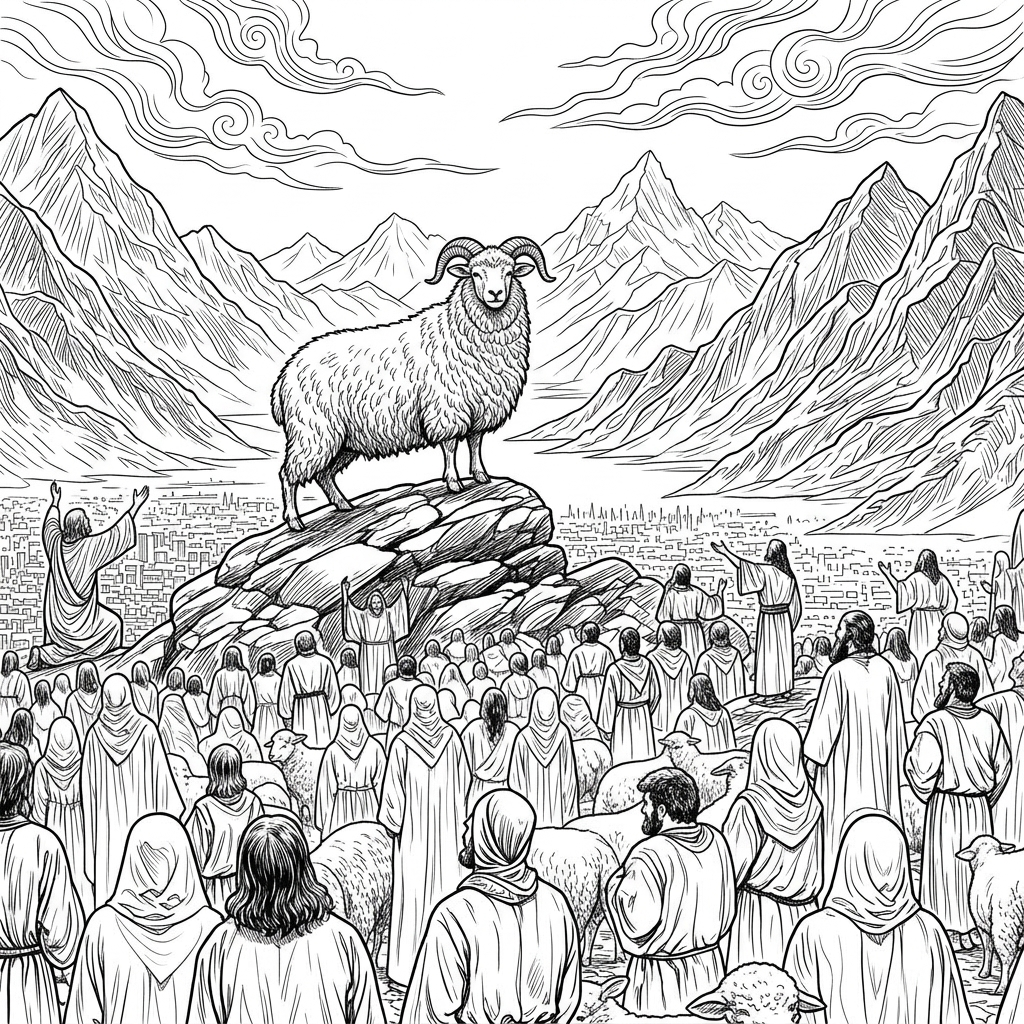
\includegraphics[
%    width=1\textwidth, 
%    trim=0 0 0 0, 
%    clip]{images/lamb_14400.jpg}
%\end{figure}


他們是「從人間買來的、作初熟的果子歸與　神和羔羊」，表示他們也是被耶穌救贖\idx{11}{救贖}的人。「在他們口中察不出謊言來．他們是沒有瑕疵的」是說在耶穌的眼中，他們是
沒有瑕疵的。
他們是「未曾沾染婦女、他們原是童身」的，可能就是獨身，沒有沾染婦女者。
因為舊約以婚姻與淫亂描寫對神忠誠或不忠，這裡表示，他們是忠誠於羔羊的人。無論羔羊往那裡去、他們都跟隨他。

\begin{ReaderQuestion}
「羔羊無論往那裡去，他們都跟隨他」（14:4）對你而言意味著什麼？
\end{ReaderQuestion}

他們的歌，有天地間的獨特。是只有親身走過救贖之路、在考驗中堅定跟隨羔羊的人，才能從靈魂深處唱出的生命讚美。沒有人能學他們的新歌。

\section{天使傳永遠的福音}

\begin{ScriptureBox2}{劃出三位天使各自宣告的內容。14:13中誰是有福的？為什麼？}


\item[14:6] 我又看見另有一位天使飛在空中、有永遠的福音要傳給住在地上的人、就是各國各族各方各民．

\item[14:7] 他大聲說、應當敬畏　神、將榮耀歸給他．因他施行審判的時候已經到了．應當敬拜那創造天地海和眾水泉源的。

\item[14:8] 又有第二位天使、接著說、叫萬民喝邪淫大怒之酒的巴比倫大城傾倒了、傾倒了。

\item[14:9] 又有第三位天使、接著他們、大聲說、若有人拜獸和獸像、在額上、或在手上、受了印記、

\item[14:10] 這人也必喝　神大怒的酒、此酒斟在　神忿怒的杯中純一不雜．他要在聖天使和羔羊面前、在火與硫磺之中受痛苦．

\item[14:11] 他受痛苦的煙往上冒、直到永永遠遠．那些拜獸和獸像受他名之印記的、晝夜不得安寧。

\item[14:12] 聖徒的忍耐就在此．他們是守　神誡命、和耶穌真道的。

\item[14:13] 我聽見從天上有聲音說、你要寫下、從今以後、在主裡面而死的人有福了．聖靈說、是的、他們息了自己的勞苦、作工的果效也隨著他們。

\end{ScriptureBox2}

\begin{figure}[h]
    \centering
    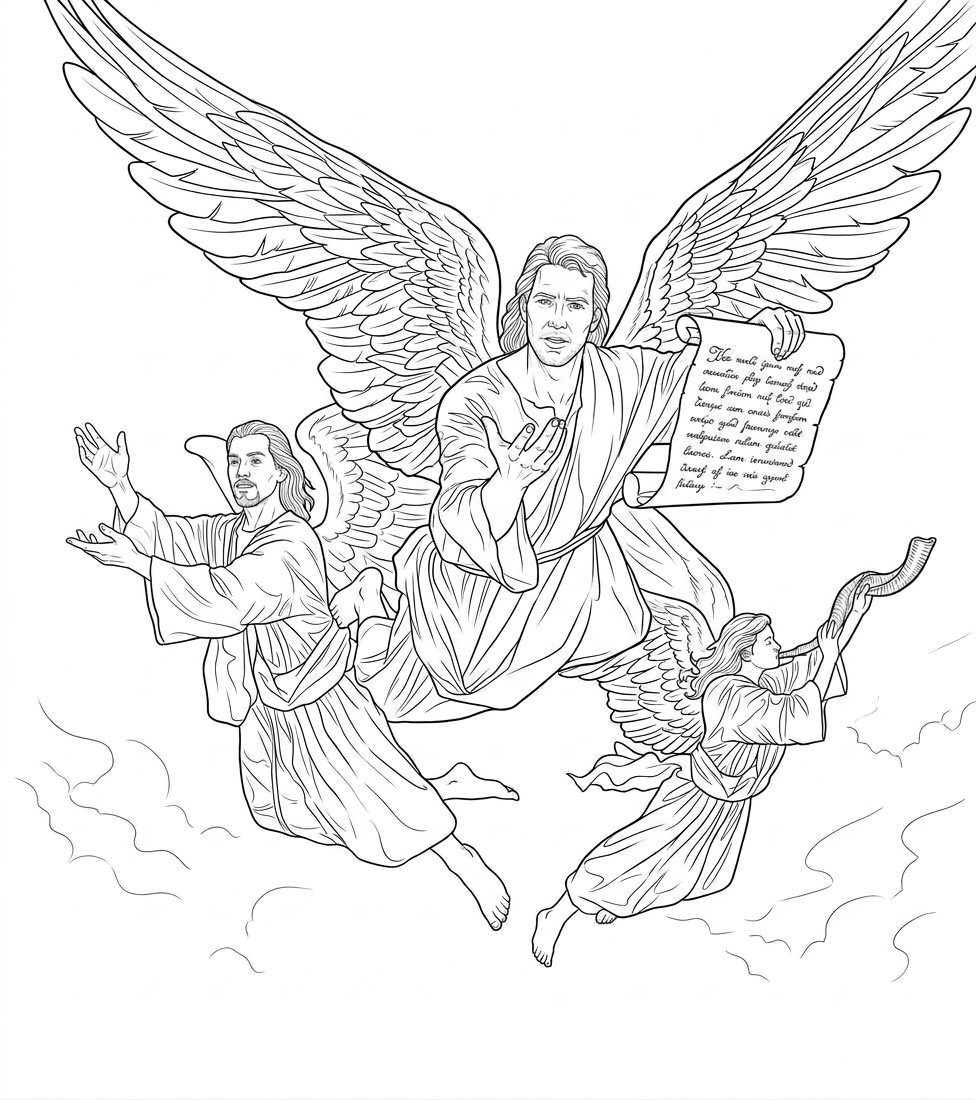
\includegraphics[
    width=0.8\textwidth, 
    trim=0 0 0 0, 
    clip]{images/eternal_gospel.jpg}
\end{figure}

到了這個時候，天上仍然有福音傳給地上的人。這福音是什麼呢？就是人應當要「敬畏神，將榮耀\idx{14}{榮耀}歸給他」，要敬拜祂，因為祂是「創造天地海和眾水泉源的。」
人受造，就是生命的恩典\idx{10}{恩典}，人敬拜神並歸榮耀與神，是受造之人應當對造物主回應。

\begin{ReaderQuestion}
第一位天使所宣告的「永遠的福音」包括哪些內容？（14:6–7）為什麼「敬畏神、將榮耀歸給祂、敬拜創造主」與福音的信息有關？
\end{ReaderQuestion}

接著其他兩位天使宣判公義的審判\idx{15}{審判}。悖逆的受造之人不只拒絕受造之恩典，
拒絕耶穌的救贖\idx{11}{救贖}的寶血，
而且拜獸，在手上接受印記，逼迫\idx{13}{逼迫}聖徒。所以拜獸之人受痛苦，直到永永遠遠，這樣的審判豈不公義嗎？

而忍耐持守的人，在主裡面而死的人，有福了。他們真的息了自己的勞苦，他們一生為主做工的果效也隨著他們，這是多大的安慰！

\section{兩幅收割的異象}


\begin{ScriptureBox2}{比較這兩次收割。誰揮出第一把鐮刀？第二次收割收取的是什麼？又被丟在哪裡？}

\item[14:14] 我又觀看、見有一片白雲、雲上坐著一位好像人子、頭上戴著金冠冕、手裡拿著快鐮刀。

\item[14:15] 又有一位天使從殿中出來、向那坐在雲上的大聲喊著說、伸出你的鐮刀來收割．因為收割的時候已經到了、地上的莊稼已經熟透了。

\item[14:16] 那坐在雲上的、就把鐮刀扔在地上．地上的莊稼就被收割了。

\item[14:17] 又有一位天使從天上的殿中出來、他也拿著快鐮刀。

\item[14:18] 又有一位天使從祭壇中出來、是有權柄管火的、向拿著快鐮刀的大聲喊著說、伸出快鐮刀來收取地上葡萄樹的果子．因為葡萄熟透了。

\item[14:19] 那天使就把鐮刀扔在地上、收取了地上的葡萄、丟在　神忿怒的大酒醡中。

\item[14:20] 那酒醡踹在城外、就有血從酒醡裡流出來、高到馬的嚼環、遠有六百里。

\end{ScriptureBox2}

前面幾章我們已經講過，這裡的「人子\idx{02}{人子}」就是耶穌基督。莊稼已經熟了，所以祂手裡拿著快鐮刀要收割\idx{06}{收割}了。
耶穌在約翰福音4:35說：「你們豈不說、到收割的時候、還有四個月麼．我告訴你們、舉目向田觀看、莊稼已經熟了、〔原文作發白〕可以收割了。」
滿滿金黃色的麥子低垂，工人們拿著快鐮刀收割，這是多麼快樂的場景！

收割的時候，也是審判\idx{15}{審判}的時候。工人們會將麥子和稗子分別開來，麥子收在倉裡，稗子燒掉。
這就是主耶穌在馬太福音13:24-30，用農家最能夠了解的比喻，
農夫不需要在幼苗的時候就分別麥子和稗子。要容許這兩樣一齊長。在收割的時候，就可以分別出來。\footnote{馬太福音13:24-30：「耶穌又設個比喻對他們說、天國好像人撒好種在田裡．
及至人睡覺的時候、有仇敵來、將稗子撒在麥子裡、就走了。
到長苗吐穗的時候、稗子也顯出來。
田主的僕人來告訴他說、主阿、你不是撒好種在田裡麼、從那裡來的稗子呢。
主人說、這是仇敵作的。僕人說、你要我們去薅出來麼。
主人說、不必、恐怕薅稗子、連麥子也拔出來。
容這兩樣一齊長、等著收割．當收割的時候、我要對收割的人說、先將稗子薅出來、捆成捆、留著燒．惟有麥子、要收在倉裡。」}

收割和審判，在約珥書3:13講的明明白白：「開鐮罷．因為莊稼熟了．踐踏罷。因為酒醡滿了、酒池盈溢．他們的罪惡甚大。」
啟示錄這裡有天使把鐮刀扔在地上，是要收取地上的葡萄，然後丟在神忿怒的大酒醡中。審判的時候到了。
審判罪大惡極的惡人，就像醡葡萄酒一樣，酒池盈溢流出，竟然高至馬的嚼環，遠達六百里。

\begin{ReaderQuestion}
啟示錄14章呈現兩次收割：人子收割的莊稼，以及被丟在神忿怒大酒醡中的葡萄。既然最後的收割還沒有來到，神今天的忍耐應當如何影響你回應祂的方式，以及你向別人談論祂的方式？
\end{ReaderQuestion}

\begin{figure}[htbp]
    \centering
    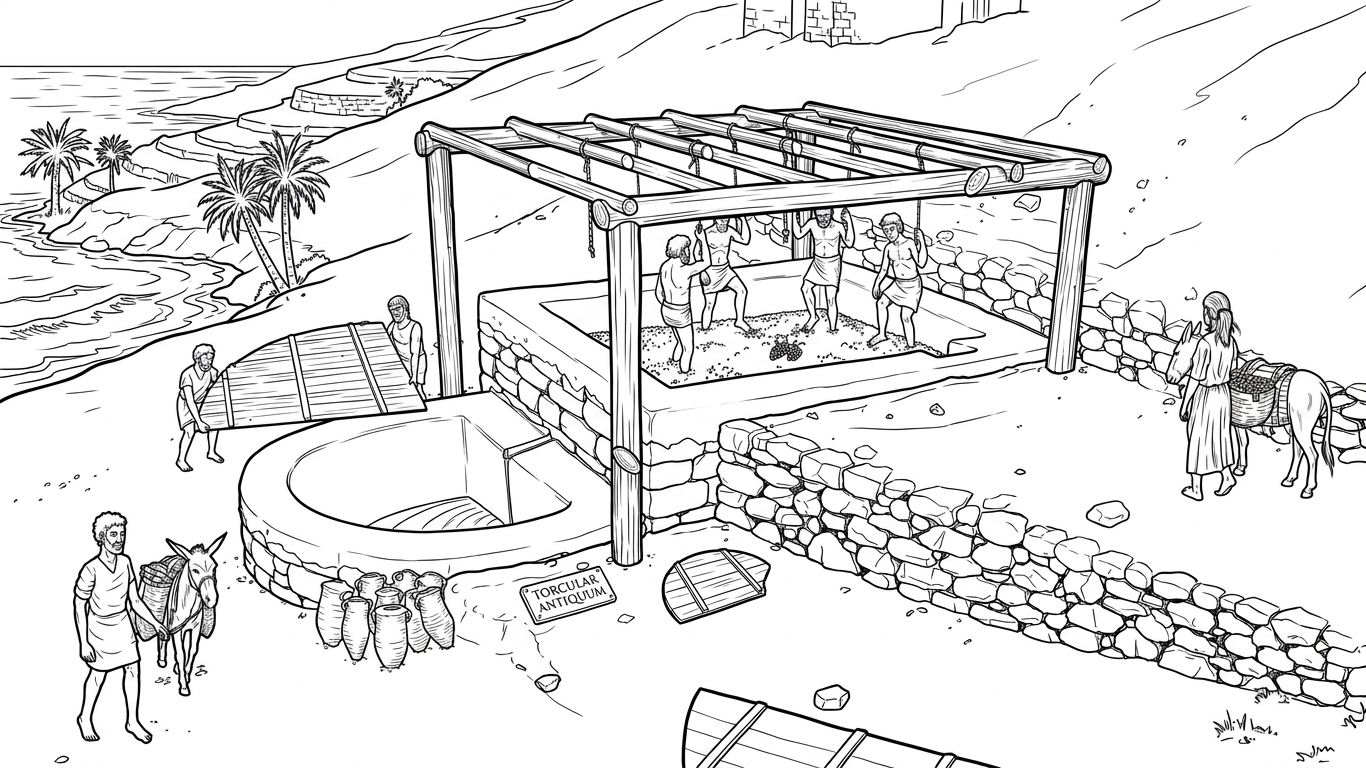
\includegraphics[
    width=1\textwidth, 
    trim=0 0 0 0, 
    clip]{images/wine_pressing.jpg}
\end{figure}

\chapter{神完全的憤怒施行公義審判（15:1-16:21）}

如果說前面的七印與七號讓我們逐步看見神的審判，那麼到了啟示錄第15、16章，審判進入最後的階段。約翰看見七位天使掌管末了的七災，並將七個金碗盛滿神的忿怒，傾倒在地上。

在可怕的審判之前，約翰先讓我們看見一幅得勝的畫面：那些勝過獸、勝過獸的像和牠名字數目的人，站在玻璃海上，手拿著神的琴，唱著「摩西的歌，又唱羔羊的歌」。這個安排非常重要。審判臨到之前，約翰先讓我們看見得勝的教會。屬於羔羊的人不是在神的忿怒之下，而是在祂的保守中。他們經過患難，卻並沒有向獸屈服，所以最終站在神面前歡喜的敬拜祂。

\section{唱羔羊的新歌}

\begin{ScriptureBox2}{圈出站在玻璃海上的人手裡拿著什麼，以及他們唱的是誰的歌。劃出15:3中描述神的作為和道途的字句。}
\item[15:1] 我又看見在天上有異象、大而且奇、就是七位天使掌管末了的七災．因為　神的大怒在這七災中發盡了。

\item[15:2] 我看見彷彿有玻璃海、其中有火攙雜．又看見那些勝了獸和獸的像、並他名字數目的人、都站在玻璃海上、拿著　神的琴．

\item[15:3] 唱　神僕人摩西的歌、和羔羊的歌、說、主　神、全能者阿、你的作為大哉、奇哉、萬世之王阿、〔世或作國〕你的道途義哉、誠哉。

\item[15:4] 主阿、誰敢不敬畏你、不將榮耀歸與你的名呢．因為獨有你是聖的．萬民都要來在你面前敬拜．因你公義的作為已經顯出來了。

\item[15:5] 此後、我看見在天上那存法櫃的殿開了．

\item[15:6] 那掌管七災的七位天使、從殿中出來、穿著潔白光明的細麻衣、〔細麻衣有古卷作寶石〕胸間束著金帶。

\item[15:7] 四活物中有一個把盛滿了活到永永遠遠之　神大怒的七個金碗給了那七位天使。

\item[15:8] 因　神的榮耀、和能力、殿中充滿了煙．於是沒有人能以進殿、直等到那七位天使所降的七災完畢了。
\end{ScriptureBox2}

\begin{InDepth}
\InDepthHeading{摩西的歌與羔羊的歌}

啟示錄15章與出埃及記15章有明顯對照。如表\ref{tab:rev_exdus_15}。當摩西與百姓過紅海，法老及埃及軍隊被淹沒在紅海裡。摩西與百姓雀躍，唱新歌。到了啟示錄15章，是羔羊救贖祂的百姓、勝過一切敵對勢力的終極勝利之歌。

\par\medskip\noindent
\begin{minipage}{\linewidth}
\centering\small
\renewcommand{\arraystretch}{1}\setlength{\tabcolsep}{4pt}
\captionof{table}{啟示錄15章與出埃及記15章}
\label{tab:rev_exdus_15}
\begin{tabularx}{\linewidth}{@{}>{\raggedright\arraybackslash}X
                               >{\raggedright\arraybackslash}X
                               >{\raggedright\arraybackslash}X@{}}
\hline
啟示錄15 & 出埃及15 & 內容 \\
\hline
1 七災 & 埃及十災 & 神對仇敵施行審判 \\
2 站在玻璃海上 & 過紅海 & 神拯救祂的百姓 \\
2 獸 & 法老及埃及軍隊 & 神與仇敵爭戰 \\
3 摩西的歌 & 摩西的歌 & 救贖後的勝利之歌 \\
5 存法櫃的殿 & 會幕／聖所 & 神的同在 \\
8 煙充滿殿 & 神的榮耀 & 神臨在並施行審判 \\
\hline
\end{tabularx}
\end{minipage}
\end{InDepth}

這歌唱的不是稱讚人的勇敢，而是宣告神的作為「大哉、奇哉」、「義哉、誠哉」。我們在患難中容易把注意力放在自己的處境上，這首歌使我們的眼目重新定睛在神身上。

\begin{ReaderQuestion}
啟示錄15:3-4的歌頌不是稱讚人的勇敢，而是宣告神的作為「大哉、奇哉」、「義哉、誠哉」。我們在患難中容易把注意力放在自己的處境上，這首歌如何把我們的眼目重新轉向神？
\end{ReaderQuestion}

天使接了碗去傾倒在地上。地上有災，天上有殿，直到七位天使所降的七災完畢了。

\section{第1-5碗}

\begin{figure}[htbp]
    \centering
    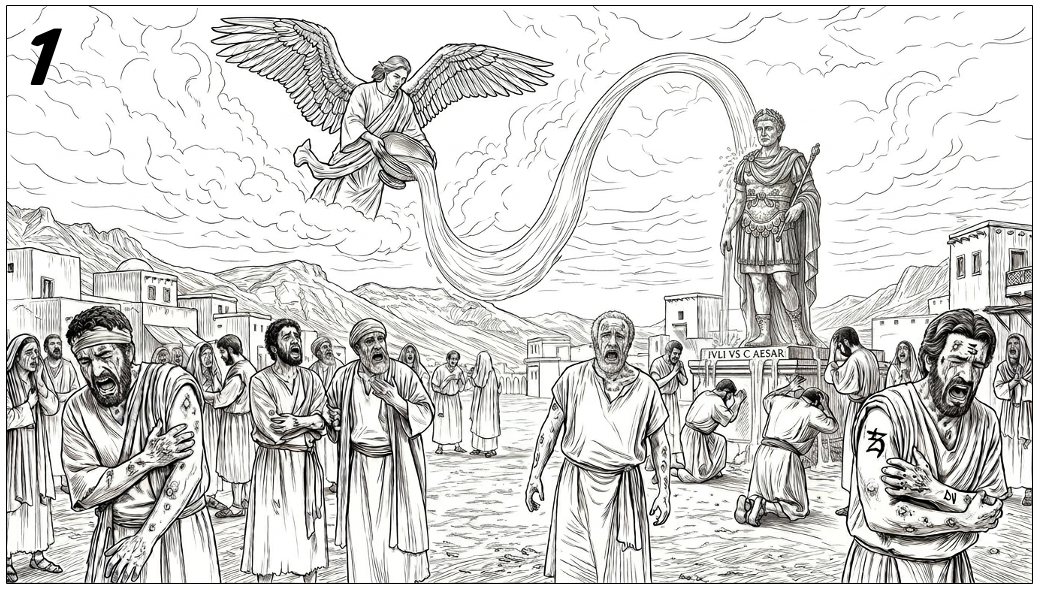
\includegraphics[
    width=1\textwidth, 
    trim=0 0 0 0, 
    clip]{images/bowl_1.png}
\end{figure}


\begin{figure}[htbp]
    \centering
    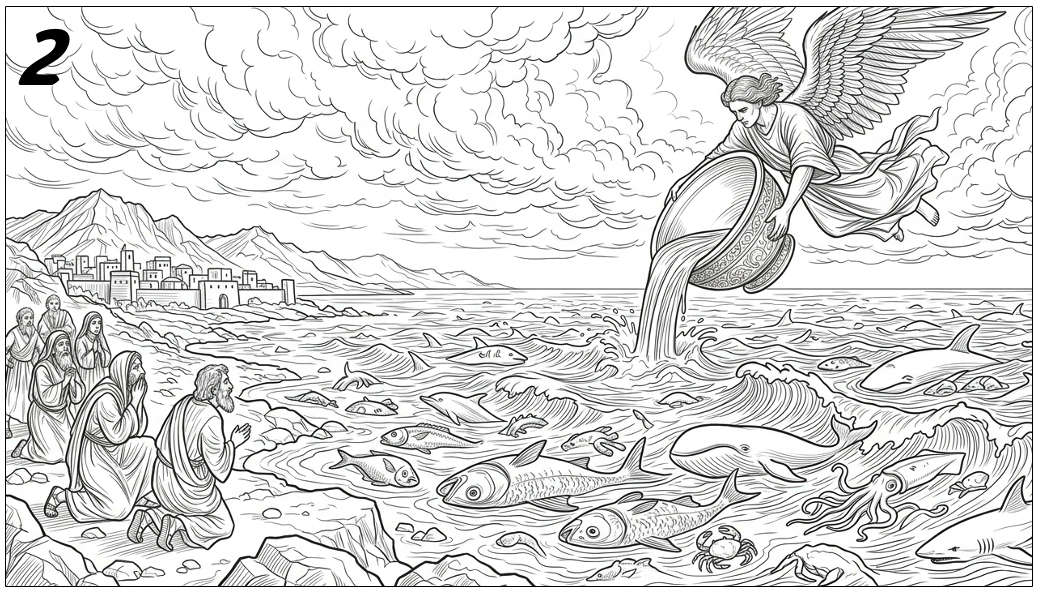
\includegraphics[
    width=1\textwidth, 
    trim=0 0 0 0, 
    clip]{images/bowl_2.png}
\end{figure}


\begin{ScriptureBox2}{前五碗各倒在哪裡？劃出16:9和16:11中人的反應。}

\item[16:1] 我聽見有大聲音從殿中出來、向那七位天使說、你們去、把盛　神大怒的七碗倒在地上。

\item[16:2] 第一位天使便去、把碗倒在地上、就有惡而且毒的瘡、生在那些有獸印記、拜獸像的人身上。

\item[16:3] 第二位天使把碗倒在海裡、海就變成血、好像死人的血．海中的活物都死了。

\item[16:4] 第三位天使把碗倒在江河與眾水的泉源裡、水就變成血了。

\item[16:5] 我聽見掌管眾水的天使說、昔在今在的聖者阿、你這樣判斷是公義的．

\item[16:6] 他們曾流聖徒與先知的血、現在你給他們血喝．這是他們所該受的。

\item[16:7] 我又聽見祭壇中有聲音說、是的、主　神、全能者阿、你的判斷義哉、誠哉。

\item[16:8] 第四位天使把碗倒在日頭上、叫日頭能用火烤人。

\item[16:9] 人被大熱所烤、就褻瀆那有權掌管這些災的　神之名、並不悔改將榮耀歸給　神。

\item[16:10] 第五位天使把碗倒在獸的座位上、獸的國就黑暗了．人因疼痛就咬自己的舌頭．

\item[16:11] 又因所受的疼痛、和生的瘡、就褻瀆天上的　神、並不悔改所行的。

\end{ScriptureBox2}

\begin{figure}[htbp]
    \centering
    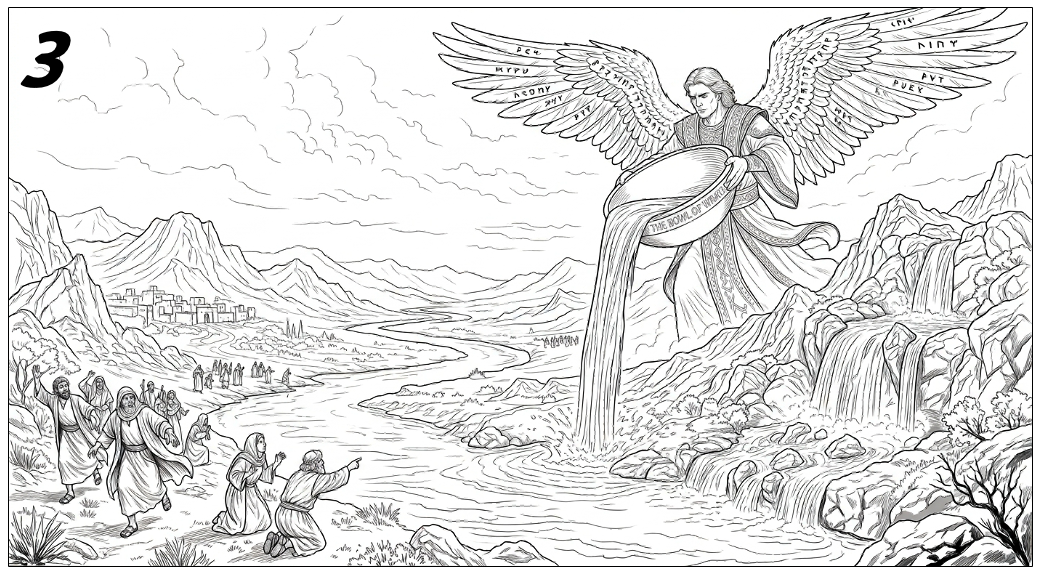
\includegraphics[
    width=1\textwidth, 
    trim=0 0 0 0, 
    clip]{images/bowl_3.png}
\end{figure}


第一碗臨到拜獸的人，第二、三碗擊打海洋與江河，第四、五碗擴大到人與獸的國，第六碗聚集末後爭戰，第七碗宣告「成了」，七碗的審判一步一步加重，直到神的忿怒完全傾倒，審判達到終局。

這些可怕的場景，不是發生在那些屬於羔羊、蒙祂救贖的人身上，而是臨到「那些有獸印記、拜獸像的人」。每一個碗都盛滿了神完全的忿怒。神曾經長久忍耐，一次又一次呼召人悔改。然而到了這裡，時間已經到了。

\begin{ReaderQuestion}
你如何理解「神的忍耐」與「神最終的審判」之間的關係？神的忍耐是否代表祂輕看罪？
\end{ReaderQuestion}


\begin{figure}[htbp]
    \centering
    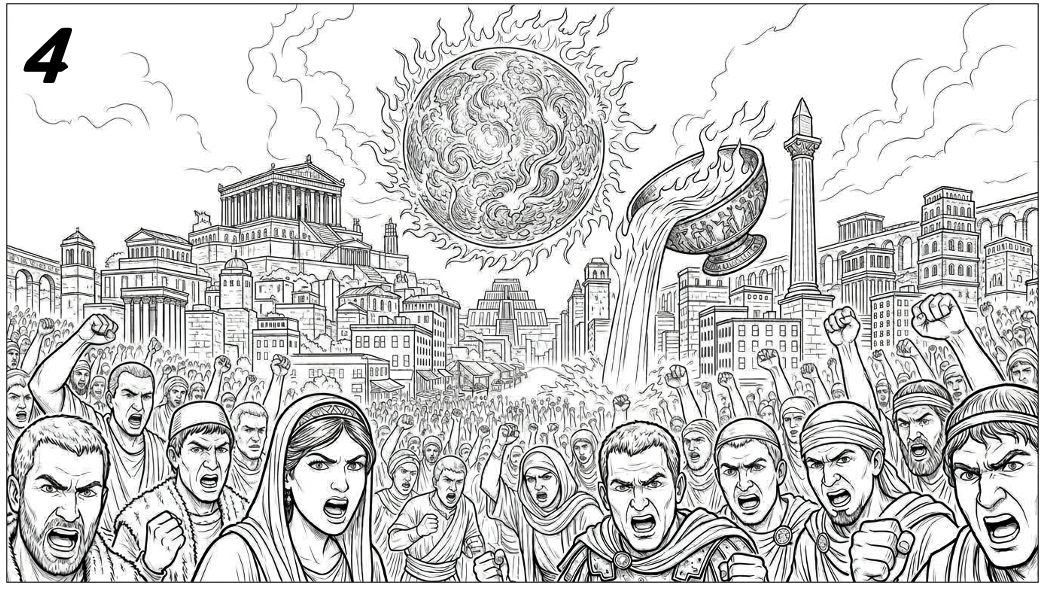
\includegraphics[
    width=1\textwidth, 
    trim=0 0 0 0, 
    clip]{images/bowl_4.png}
\end{figure}

讀到這裡，我們會想起第一冊《被恩典追上》第十章所介紹的愛德華滋（Jonathan Edwards）著名講道〈在忿怒之神手中的罪人〉（\textit{Sinners in the Hands of an Angry God}）。愛德華滋以極其強烈的語言描述尚未投靠基督的罪人所面對的危險：
\begin{quote}
「罪人啊！當仔細思量你所處可怕的危險：那是烈怒的大熔爐，寬闊無底的深淵，充滿火焰與怒氣，而你被握在那位神的手中，他對你的怒氣如同已經激怒的烈火，如同眾多地獄中的罪人一樣猛烈。你懸於纖細的線上，神聖的怒火焰環繞其周，每一刻都準備焚燒它；你沒有任何中保的幫助，無法挽救自己，無法抵禦怒火，一切自身所有、一切行為，都不能使神寬恕你一刻……」
\end{quote}

親愛的讀者，今天仍是恩典的日子。羔羊已經為罪人捨命。正因為將來的審判如此真實，神的恩典才顯得如此寶貴。你願意回應神的恩典，接受祂的救恩嗎？

\begin{ReaderQuestion}
今天仍是恩典的日子。你認為自己應當如何更認真地悔改、持守信仰、仰望羔羊，並向還沒有認識基督的人傳福音？
\end{ReaderQuestion}

\begin{figure}[htbp]
    \centering
    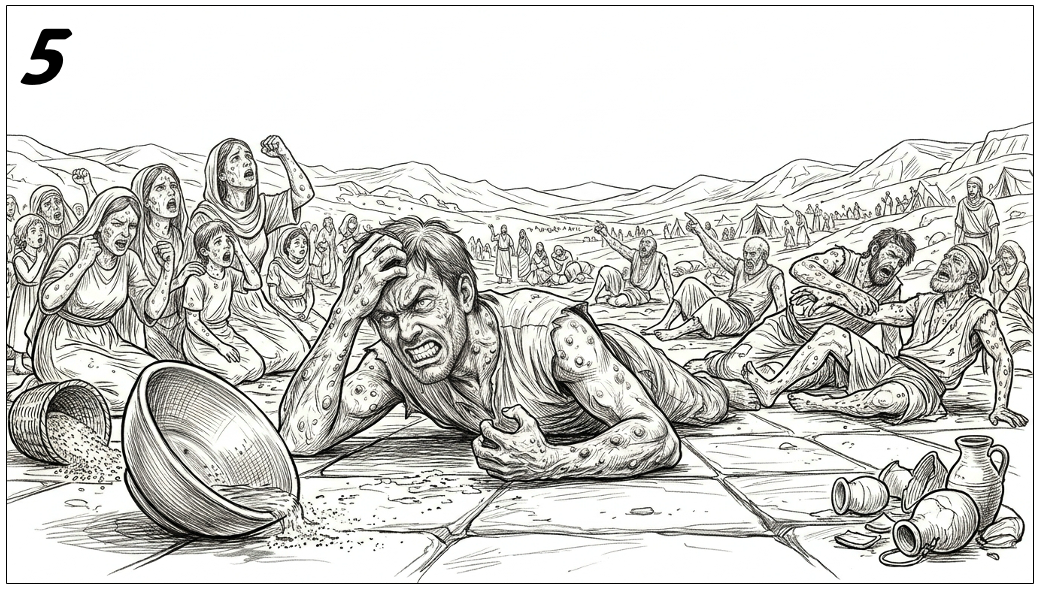
\includegraphics[
    width=1\textwidth, 
    trim=0 0 0 0, 
    clip]{images/bowl_5.png} 
\end{figure}


\section{第六碗}

\begin{ScriptureBox2}{三個污穢的靈從誰的口中出來？他們聚集眾王要做什麼？耶穌在16:15說了什麼祝福？}

\item[16:12] 第六位天使把碗倒在伯拉大河上、河水就乾了、要給那從日出之地所來的眾王預備道路。

\item[16:13] 我又看見三個污穢的靈、好像青蛙、從龍口獸口並假先知的口中出來．

\item[16:14] 他們本是鬼魔的靈、施行奇事、出去到普天下眾王那裡、叫他們在　神全能者的大日聚集爭戰。

\item[16:15] （看哪、我來像賊一樣。那儆醒、看守衣服、免得赤身而行、叫人見他羞恥的、有福了。）

\item[16:16] 那三個鬼魔便叫眾王聚集在一處、希伯來話叫作「哈米吉多頓。」

\end{ScriptureBox2}

\begin{figure}[htbp]
    \centering
    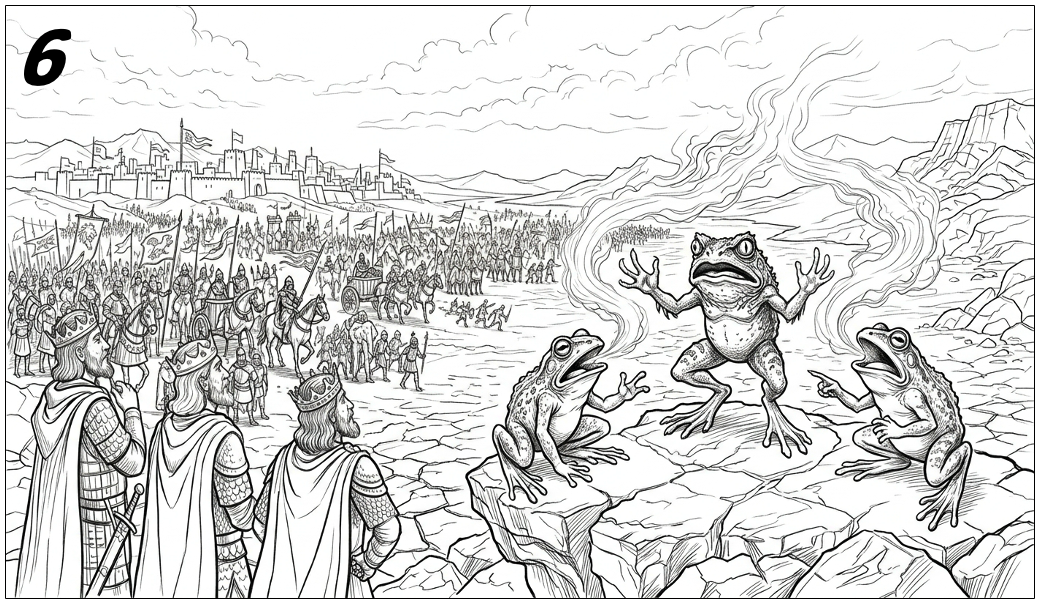
\includegraphics[
    width=1\textwidth, 
    trim=0 0 0 0, 
    clip]{images/bowl_6.png} 
\end{figure}


這一節是七碗審判的高潮之一。
從龍、獸和假先知口中出來、形狀像青蛙的三個污穢的靈，唆使世上的君王聚集。這些列國的君王以為自己正在作自己的政治與軍事決定，然而約翰從屬靈的角度看見，他們受到邪靈的迷惑，正被聚集到神最後的審判之中。

「哈米吉多頓」(Armageddon)在許多末世小說與電影中被當做末日大戰的場景。這個名稱通常與希伯來文的米吉多（Megiddo）有關。
米吉多是古代以色列的重要戰略地區，也是多場戰爭的所在地。因此很自然成為約翰描寫末日衝突的象徵性背景。

啟示錄 16:16 描述敵對神的地上勢力被唆使聚集到「哈米吉多頓」，而真正的哈米吉多頓戰役場景是在後面的 啟示錄 19:19–21。此哈米吉多頓戰役也不是兩個勢均力敵的陣營，是基督完全得勝。
\begin{InDepth}
\InDepthHeading{啟示錄16章與19章的關聯}

因為經文橫跨兩章，我用圖\ref{rev_16_19_armageddon_chinese}表示。此圖也使我們看到，是撒旦透過三隻污穢的青蛙，唆使隨從他的人類來攻擊神。只是他也知道「自己的時候不多、就氣忿忿的下到你們那裡去了。」（啟示錄12:12）

\par\medskip\noindent
\begin{minipage}{\linewidth}
\centering
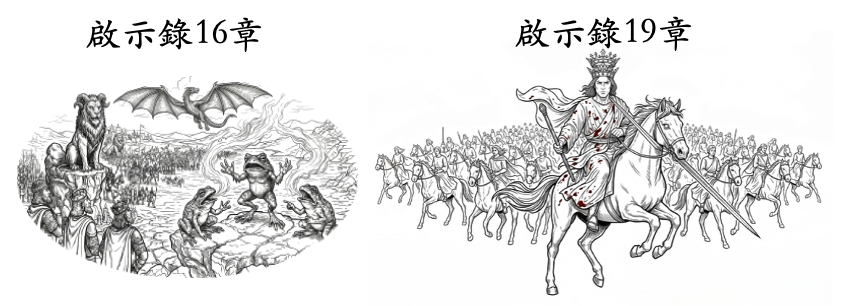
\includegraphics[
    width=\linewidth,
    trim=0 10 20 0,
    clip]{images/rev_16_19_armageddon_chinese.png}
\captionof{figure}{哈米吉多頓的戰役}
\label{rev_16_19_armageddon_chinese}
\end{minipage}
\end{InDepth}

\section{第七碗}

\begin{ScriptureBox2}{寶座上的大聲音宣告什麼？圈出接著發生的每一個現象，並留意人對雹災的反應。}

\item[16:17] 第七位天使把碗倒在空中、就有大聲音從殿中的寶座上出來、說、成了．

\item[16:18] 又有閃電、聲音、雷轟、大地震、自從地上有人以來、沒有這樣大這樣利害的地震。

\item[16:19] 那大城裂為三段、列國的城也都倒塌了．　神也想起巴比倫大城來、要把那盛自己烈怒的酒杯遞給他。

\item[16:20] 各海島都逃避了、眾山也不見了。

\item[16:21] 又有大雹子從天落在人身上、每一個約重一他連得．〔一他連得約有九十斤〕為這雹子的災極大、人就褻瀆　神。

\end{ScriptureBox2}

這裡最重要的是神說「成了」。神的審判已經完成，但人的悖逆直到最後仍然沒有改變。

這樣的地震，是有人類以來，沒有經歷過的地震。雹重90斤，約是45公斤，或是100英鎊。
但人仍然「褻瀆神」。

讀到這裡，讓我們想起第一冊「被恩典追上」12章曾經引用魯益師（C.S. Lewis）在其著作《大分裂》說的：
\begin{quote}
「到最後，人只分為兩種：一種是對神說「願你的旨意成就」的人。另一種是最後由神對他們說「願你的己意成就」的人。」—魯益師（C.S. Lewis）\footnote{“There are only two kinds of people in the end: those who say to
God, ”Thy will be done,” and those to whom God says, in the end,
”Thy will be done.” All that are in Hell, choose it. Without that
self-choice there could be no Hell. No soul that seriously and
constantly desires joy will ever miss it. Those who seek find. Those
who knock it is opened.” Lewis, C. S. (1946). \textit{The great divorce.}
Geoffrey Bles.}
\end{quote}

\begin{ReaderQuestion}
魯益師說，到最後人只分為兩種：一種是對神說「願你的旨意成就」的人，另一種是最後由神對他們說「願你的己意成就」的人。在你生命中的哪一個領域，你仍然緊抓著自己的意思？今天對神說「願你的旨意成就」，會是什麼樣子？
\end{ReaderQuestion}

\section*{七碗的特徵}

{
\small
\renewcommand{\arraystretch}{1}
\begin{longtable}{p{1.5cm} p{2cm} p{2cm}}
\caption{七碗審判口訣}
\label{tab:seven-bowls-zh} \\
\hline
碗 & 經文 & 審判 \\
\hline
\endfirsthead

\multicolumn{3}{l}{\small\itshape 表~\thetable（續）} \\
\hline
碗 & 經文 & 審判 \\
\hline
\endhead

\hline
\endfoot

\hline
\endlastfoot

第一碗 & 16:1--2 & 惡毒瘡 \\
第二碗 & 16:3 & 海變血 \\
第三碗 & 16:4--7 & 河變血 \\
第四碗 & 16:8--9 & 日火烤 \\
第五碗 & 16:10--11 & 痛咬舌 \\
第六碗 & 16:12--16 & 集爭戰 \\
第七碗 & 16:17--21 & 成了 \\
\end{longtable}
}

\chapter{巴比倫傾倒，羔羊得勝（17:1-18:24）}

巴比倫代表奢華、權勢與經濟利益引誘世人的世界體系。

約翰看見一個穿著華美、坐在朱紅色獸上的女人，她擁有金子、寶石和珍珠。她與地上的君王聯合，使列國沉醉，也使地上的客商因她的奢華而發財。她華麗的外表之下，隱藏著罪惡、偶像、淫亂、驕傲，以及她對神子民的逼迫。她看似強大、富足、不可撼動，神卻宣告她終必傾倒。

巴比倫最危險的地方，不只是她公開敵對神，而是她具有極大的吸引力。她以財富、成功、權勢、奢華和享樂吸引人，使人以為這就是人生所應追求的榮耀。她不一定要求人立刻否認神；她更可能使人慢慢把安全感放在財富，把價值建立在成功，把盼望寄託在權勢，把滿足建立在物質上。

因此，巴比倫的信息不只是給末世的讀者，也是給今天每一個活在世界中的基督徒。

我們工作、經商、使用金錢、科技和社會資源，是神所賜的美好事物。
而且我們不能離開世界而生活。
問題不是我們是否使用這些東西，而是我們是否開始敬拜這些東西；不是我們是否擁有財富，而是財富是否開始擁有我們的心。
神不是呼召基督徒逃離世界，而是呼召我們不要被世界的價值觀同化。

所以，神對祂的百姓發出一個清楚的呼召：
「我的民哪，你們要從那城出來，免得與她一同有罪。」（啟示錄18:4）

啟示錄把兩個女人放在我們面前：一邊是坐在獸上的巴比倫，一邊是預備自己迎接羔羊的教會；一邊是地上的奢華，一邊是天上的榮耀；一邊看似強大卻轉眼傾倒，一邊在世上似乎軟弱卻永遠屬於得勝的羔羊。

願我們在這個世界中仍然忠心跟隨基督，在誘惑中持守聖潔，在物質的吸引中保持清醒，在地上的權勢面前仍然敬拜那位真正的萬王之王。

\section{巴比倫}

\begin{ScriptureBox}

\item[17:1] 拿著七碗的七位天使中、有一位前來對我說、你到這裡來、我將坐在眾水上的大淫婦所要受的刑罰指給你看．

\item[17:2] 地上的君王與他行淫．住在地上的人喝醉了他淫亂的酒。

\item[17:3] 我被聖靈感動、天使帶我到曠野去．我就看見一個女人騎在朱紅色的獸上．那獸有七頭十角、遍體有褻瀆的名號。

\item[17:4] 那女人穿著紫色和朱紅色的衣服、用金子寶石珍珠為妝飾．手拿金杯、杯中盛滿了可憎之物、就是他淫亂的污穢。

\item[17:5] 在他額上有名寫著說、奧秘哉、大巴比倫、作世上的淫婦和一切可憎之物的母。

\item[17:6] 我又看見那女人喝醉了聖徒的血、和為耶穌作見證之人的血．我看見他、就大大的希奇。

\item[17:7] 天使對我說、你為甚麼希奇呢．我要將這女人和馱著他的那七頭十角獸的奧秘告訴你。

\item[17:8] 你所看見的獸、先前有、如今沒有．將要從無底坑裡上來、又要歸於沉淪。凡住在地上名字從創世以來沒有記在生命冊上的、見先前有、如今沒有、以後再有的獸、就必希奇。

\end{ScriptureBox}


\begin{figure}[htbp]
    \centering
    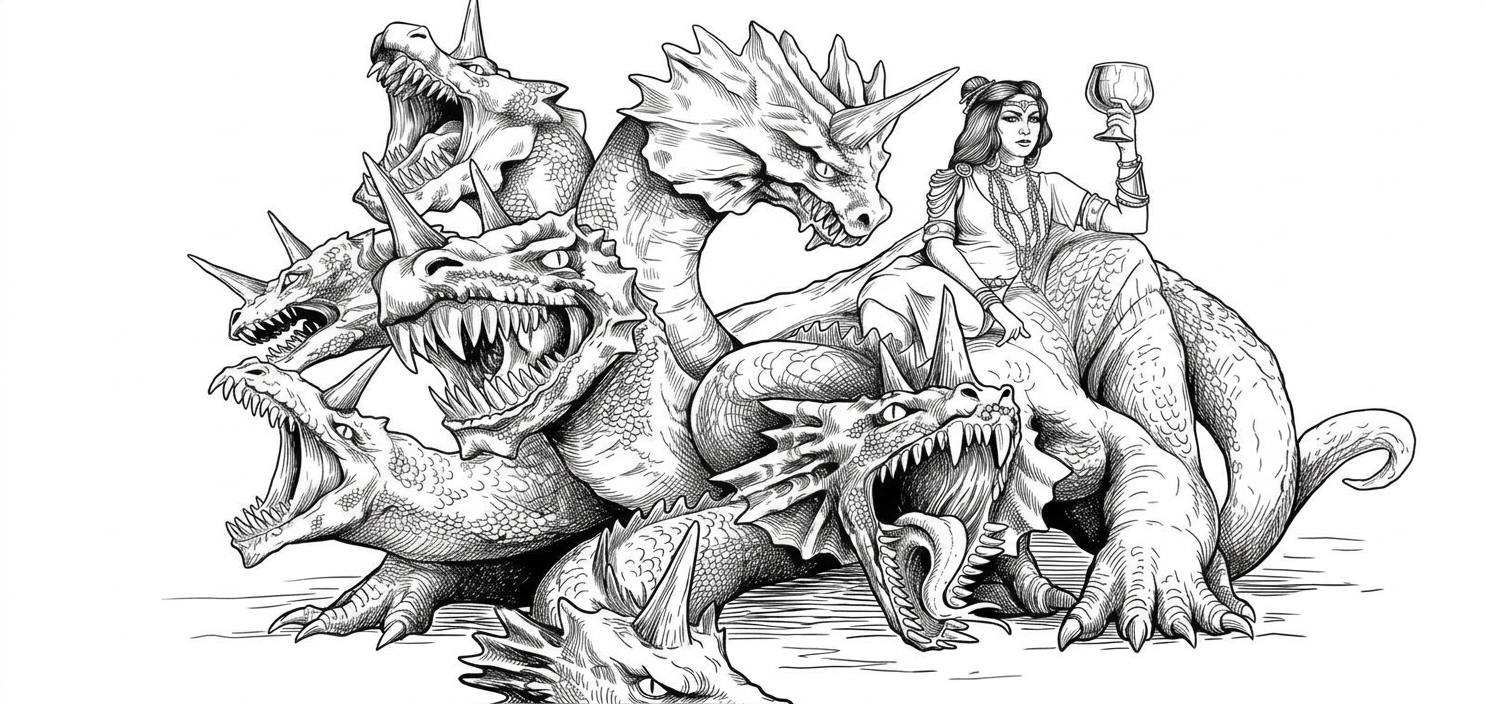
\includegraphics[
    width=1\textwidth, 
    trim=0 0 0 0, 
    clip]{images/babylon_harlot.jpg}
    %\caption{}
    %\label{}
\end{figure}




\begin{ScriptureBox}

\item[17:9] 智慧的心在此可以思想．那七頭就是女人所坐的七座山．

\item[17:10] 又是七位王．五位已經傾倒了、一位還在、一位還沒有來到．他來的時候、必須暫時存留。

\item[17:11] 那先前有、如今沒有的獸、就是第八位．他也和那七位同列、並且歸於沉淪。

\item[17:12] 你所看見的那十角、就是十王．他們還沒有得國．但他們一時之間、要和獸同得權柄與王一樣。

\item[17:13] 他們同心合意、將自己的能力權柄給那獸。

\item[17:14] 他們與羔羊爭戰、羔羊必勝過他們、因為羔羊是萬主之主、萬王之王．同著羔羊的、就是蒙召被選有忠心的、也必得勝。

\item[17:15] 天使又對我說、你所看見那淫婦坐的眾水、就是多民多人多國多方。

\item[17:16] 你所看見的那十角、與獸、必恨這淫婦、使他冷落赤身．又要喫他的肉、用火將他燒盡。

\item[17:17] 因為　神使諸王同心合意、遵行他的旨意、把自己的國給那獸、直等到　神的話都應驗了。

\item[17:18] 你所看見的那女人、就是管轄地上眾王的大城。

\end{ScriptureBox}

「巴比倫」可以解釋成第一世紀的羅馬，或是廣泛的敵對神之世界體系。因此，歷來解經家對「巴比倫」「十王」的具體身分有不同理解。
我列表出對這十王的主要解釋於表\ref{tab:ten-kings-zh} ：

{
\renewcommand{\arraystretch}{1}
\small
\begin{longtable}{p{3.6cm} p{5.4cm}}
\caption{「十王」的不同解釋（啟示錄17章）}
\label{tab:ten-kings-zh} \\
\hline
「十王」的解釋 &
主要依據 \\
\hline
\endfirsthead

\multicolumn{2}{l}{\small\itshape 表~\thetable（續）} \\
\hline
「十王」的解釋 &
主要依據 \\
\hline
\endhead

\hline
\endfoot

\hline
\endlastfoot

末世十個政治勢力的聯盟 &
17:12--13。 \\
第一世紀羅馬歷史中的十位皇帝 &
17:10「五位已經傾倒、一位還在、一位還沒有來到」。 \\
但以理書中的帝國 &
強調但以理書7章四獸與十角的背景。 \\
象徵的政治權勢 &
著重啟示錄的象徵語言，不一定是十位確定的君王。 \\
\end{longtable}
}

無論採取哪一種理解，此章的主要信息都是，這些地上的權勢最終要與羔羊爭戰，但「羔羊必勝過他們，因為羔羊是萬主之主、萬王之王」。

\section{你們要從那城出來、免得與他一同有罪}

\begin{ScriptureBox}

\item[18:1] 此後、我看見另有一位有大權柄的天使從天降下．地就因他的榮耀發光。

\item[18:2] 他大聲喊著說、巴比倫大城傾倒了、傾倒了、成了鬼魔的住處、和各樣污穢之靈的巢穴、〔或作牢獄下同〕並各樣污穢可憎之雀鳥的巢穴。

\item[18:3] 因為列國都被他邪淫大怒的酒傾倒了．地上的君王與他行淫、地上的客商、因他奢華太過就發了財。

\item[18:4] 我又聽見從天上有聲音說、我的民哪、你們要從那城出來、免得與他一同有罪、受他所受的災殃．

\item[18:5] 因他的罪惡滔天他的不義　神已經想起來了。

\item[18:6] 他怎樣待人、也要怎樣待他、按他所行的加倍的報應他．用他調酒的杯、加倍的調給他喝。

\item[18:7] 他怎樣榮耀自己、怎樣奢華、也當叫他照樣痛苦悲哀．因他心裡說、我坐了皇后的位、並不是寡婦、決不至於悲哀。

\item[18:8] 所以在一天之內、他的災殃要一齊來到、就是死亡、悲哀、饑荒、他又要被火燒盡了．因為審判他的主　神大有能力。

\item[18:9] 地上的君王、素來與他行淫一同奢華的、看見燒他的煙、就必為他哭泣哀號．

\item[18:10] 因怕他的痛苦、就遠遠的站著說、哀哉、哀哉、巴比倫大城、堅固的城阿、一時之間你的刑罰就來到了。

\item[18:11] 地上的客商也都為他哭泣悲哀、因為沒有人再買他們的貨物了．

\item[18:12] 這貨物就是金、銀、寶石、珍珠、細麻布、紫色料、綢子、朱紅色料、各樣香木、各樣象牙的器皿、各樣極寶貴的木頭和銅、鐵、漢白玉的器皿、

\item[18:13] 並肉桂、荳蔻、香料、香膏、乳香、酒、油、細麵、麥子、牛、羊、車、馬、和奴僕、人口。

\item[18:14] 巴比倫哪、你所貪愛的果子離開了你．你一切的珍饈美味、和華美的物件、也從你中間毀滅、決不能再見了。

\item[18:15] 販賣這些貨物、藉著他發了財的客商、因怕他的痛苦、就遠遠的站著哭泣悲哀、說、

\item[18:16] 哀哉、哀哉、這大城阿、素常穿著細麻、紫色、朱紅色的衣服、又用金子、寶石、和珍珠為妝飾．

\item[18:17] 一時之間、這麼大的富厚就歸於無有了。凡船主、和坐船往各處去的、並眾水手、連所有靠海為業的、都遠遠的站著、

\item[18:18] 看見燒他的煙、就喊著說、有何城能比這大城呢。

\item[18:19] 他們又把塵土撒在頭上、哭泣悲哀、喊著說、哀哉、哀哉、這大城阿．凡有船在海中的、都因他的珍寶成了富足．他在一時之間就成了荒場。

\item[18:20] 天哪、眾聖徒眾使徒眾先知阿、你們都要因他歡喜．因為　神已經在他身上伸了你們的冤。

\item[18:21] 有一位大力的天使舉起一塊石頭、好像大磨石、扔在海裡、說、巴比倫大城、也必這樣猛力的被扔下去、決不能再見了。

\item[18:22] 彈琴、作樂、吹笛、吹號的聲音、在你中間決不能再聽見．各行手藝人在你中間決不能再遇見．推磨的聲音在你中間決不能再聽見．

\item[18:23] 燈光在你中間決不能再照耀．新郎和新婦的聲音、在你中間決不能再聽見．你的客商原來是地上的尊貴人．萬國也被你的邪術迷惑了。

\item[18:24] 先知和聖徒、並地上一切被殺之人的血、都在這城裡看見了。

\end{ScriptureBox}

地上的君王和客商看到一天之內就傾倒焚毀的巴比倫城，他們就為城哭泣哀號。
這已經是七印、七號、七碗最頂峰，他們自己隨時可以滅亡。可是他們哭泣，竟然不是為了自己，而是為了所有的財寶。
可見他們貪戀財寶的心，已經使他們忘了在大審判時自身的性命安危，只是為了財寶哭泣。


\begin{figure}[htbp]
    \centering
    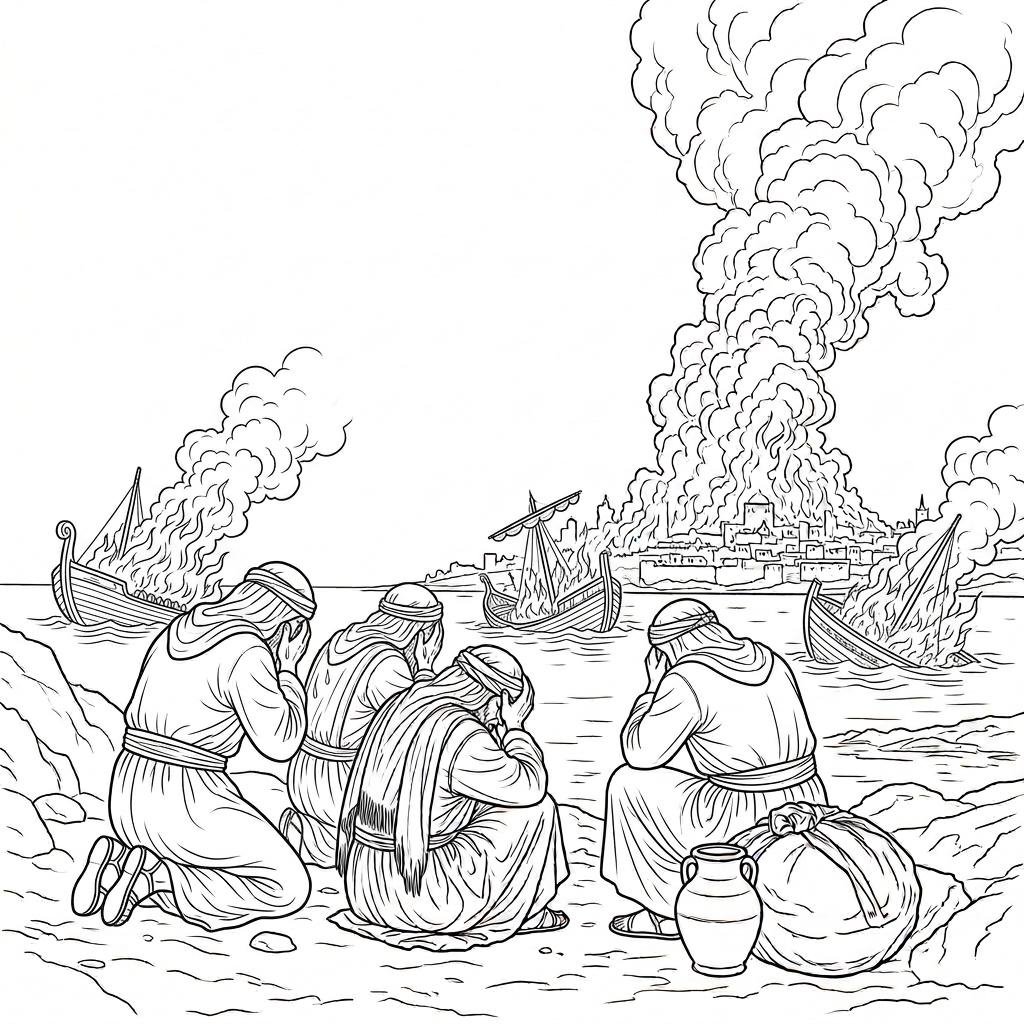
\includegraphics[
    width=1\textwidth, 
    trim=0 0 0 0, 
    clip]{images/rev_18_bablyon_burning.jpg}
    %\caption{}
    %\label{}
\end{figure}





獸代表敵對神的權勢，十角代表與獸聯合的十王，巴比倫以及大淫婦則象徵以奢華、權勢與經濟利益迷惑列國的世界體系。他們因共同的利益而聯合，將權柄交給獸，並一同敵對羔羊。最後，十角與獸反過來恨惡淫婦，使她荒涼、赤身，並焚燒她。這顯明敵對神的勢力雖能暫時結盟，卻不是永遠穩固的。神仍然掌管歷史，甚至使用他們彼此反目來成就祂的審判。

對初代教會而言，巴比倫的異象是當時信徒所面對的信仰抉擇。
因為羅馬掌握強大的政治權力，擁有龐大的商業網絡與豐富的物質資源，也以皇帝崇拜等方式彰顯其權威。
然而，當社會要求他們參與偶像崇拜，或以不符合信仰的方式表達對皇帝與地上權勢的忠誠時，他們就必須作出選擇：究竟要順從當時的社會要求，還是忠於耶穌基督？

相對於18章的巴比倫的淫婦，啟示錄21章的羔羊的新婦更是無以倫比。表\ref{tab:babylon_bride} 就顯出此對照。

{
\begin{center}
\small
\label{tab:babylon_bride}
\renewcommand{\arraystretch}{1}
\begin{longtable}{p{0.8cm} p{4.1cm} p{4.1cm}}
\caption{聖城的新婦無以倫比} \\
\hline
對比 & 巴比倫的淫婦（18章） & 聖城的新婦（21章） \\
\hline
經文 & 17:1-6；18:1-24 & 21:2, 9-10 \\

象徵 & 迷惑列國的世界體系。 & 神的子民，蒙羔羊救贖。 \\

外在 & 穿紫色和朱紅色衣服，裝飾金子、寶石、珍珠。 & 城中有神的榮耀，光輝如極貴的寶石。（11） \\

列國關係 & 地上的君王與她行淫。 & 地上的君王將榮耀歸與城（24-26） \\

與神關係 & 充滿可憎之物，並流了聖徒的血。 & 神的帳幕在人間，神要與人同住（3） \\

與人關係 & 客商因她的奢華發財。（3, 15-19） & 神白白賜生命水給口渴的人（6, 17） \\

眼淚與死亡 & 世上的人因她的毀滅而哀哭。（9-19） & 神要擦去人的眼淚，不再有死亡、悲哀、哭號、疼痛（4） \\
結局 & 毀滅（8-10, 21） & 從天而降，永遠與神同住（2-3） \\

\hline
\end{longtable}
\end{center}
}

\section*{小組討論題}

\begin{enumerate}
    \item 巴比倫外表華美、富足，卻充滿罪惡並逼迫聖徒。這個對比如何提醒我們，不要只憑外在的繁榮判斷一個社會或體系？

    \item 神說：「我的民哪，你們要從那城出來，免得與她一同有罪。」這句話對初代教會有什麼意義？對今日教會又有什麼提醒？

    \item 今天的信徒可能在哪些方面受到巴比倫的價值觀吸引？例如財富、成功、權勢、享樂或人的肯定。我們如何察驗自己的心？


\end{enumerate}

\chapter{筵席的邀約（19:1-19:21）}

啟示錄十九章把我們帶到兩個截然不同的「筵席」面前。一方面，是羔羊的婚筵\idx{10}{羔羊的婚筵}：「凡被請赴羔羊\idx{10}{羔羊}之婚筵的有福了。」羔羊的新婦\idx{13}{新婦}已經預備好了，天上充滿讚美。這是羔羊與祂子民的筵席，象徵救恩、喜樂與永恆的團契。

另一方面，卻有「神的大筵席\idx{10}{神的大筵席}」。這個筵席，飛鳥被召聚，是給飛鳥吃盡那些敵對神之人的肉。

隨後，騎白馬\idx{05}{白馬}的基督顯現。祂名為「誠信真實」，按著公義審判\idx{15}{審判}、爭戰，擊潰獸和假先知\idx{11}{假先知}。這位曾經被世人拒絕、逼迫\idx{13}{逼迫}的基督，顯明祂的榮耀\idx{14}{榮耀}，一切敵對神的勢力，在祂面前都不能站立。

今天，羔羊仍然發出祂的邀請。願我們以信心接受祂的恩典\idx{10}{恩典}，忠心跟隨祂，預備自己迎接那位即將再來的君王。

\section{羔羊之婚筵}

\begin{ScriptureBox2}{數一數「哈利路亞」出現了幾次。群眾為什麼讚美神？新婦蒙恩得穿什麼？}

\item[19:1] 此後、我聽見好像群眾在天上大聲說、哈利路亞、〔就是要讚美耶和華的意思〕救恩、榮耀、權能、都屬乎我們的　神．

\item[19:2] 他的判斷是真實公義的．因他判斷了那用淫行敗壞世界的大淫婦、並且向淫婦討流僕人血的罪、給他們伸冤。

\item[19:3] 又說、哈利路亞。燒淫婦的煙往上冒、直到永永遠遠。

\item[19:4] 那二十四位長老與四活物、就俯伏敬拜坐寶座的　神、說、阿們、哈利路亞。

\item[19:5] 有聲音從寶座出來說、　神的眾僕人哪、凡敬畏他的、無論大小、都要讚美我們的　神。

\item[19:6] 我聽見好像群眾的聲音、眾水的聲音、大雷的聲音、說、哈利路亞．因為主我們的　神、全能者、作王了。

\item[19:7] 我們要歡喜快樂、將榮耀歸給他．因為羔羊婚娶的時候到了、新婦也自己預備好了。

\item[19:8] 就蒙恩得穿光明潔白的細麻衣、這細麻衣就是聖徒所行的義。

\item[19:9] 天使吩咐我說、你要寫上、凡被請赴\textbf{羔羊之婚筵}的有福了。又對我說、這是　神真實的話。

\item[19:10] 我就俯伏在他腳前要拜他。他說、千萬不可．我和你並你那些為耶穌作見證的弟兄同是作僕人的．你要敬拜　神．因為預言中的靈意、乃是為耶穌作見證。

\end{ScriptureBox2}

天上的群眾讚美神，因為神的判斷是真實公義的。神公義完全彰顯，所以他們的讚美。這裡包含了6:10殉道\idx{10}{殉道}者。他們曾經問：「聖潔真實的主啊，你不審判\idx{15}{審判}住在地上的人，給我們伸流血的冤，要等到幾時呢？」

\begin{ReaderQuestion}
19:9說「凡被請赴羔羊之婚筵的有福了」。如果我們真正相信自己是被邀請赴羔羊婚筵的人，今天的生活態度應該有什麼不同？
\end{ReaderQuestion}

\section{騎白馬的基督：萬王之王}


\begin{figure}[htbp]
    \centering
    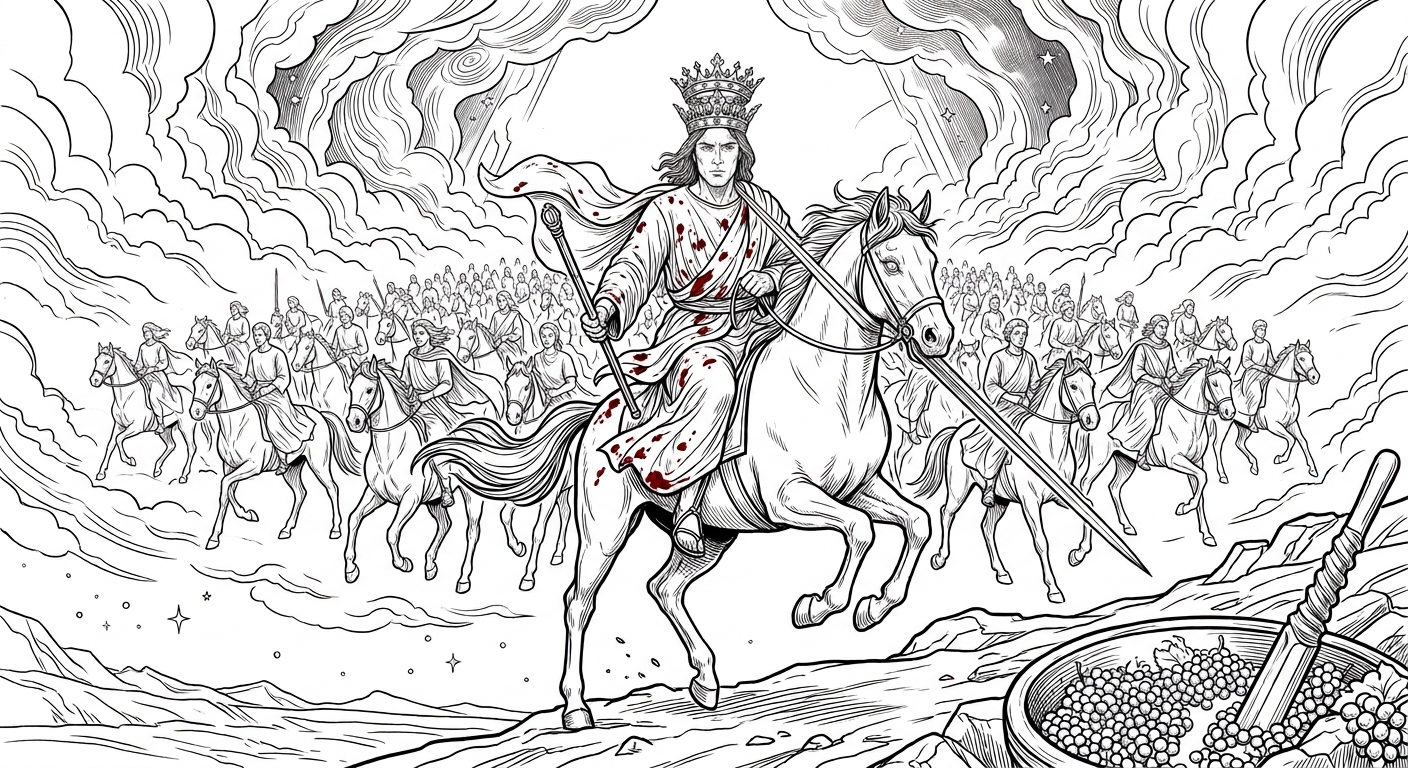
\includegraphics[
    width=1\textwidth, 
    trim=0 0 0 0, 
    clip]{images/christ_blood_white_horse.jpg}
    %\caption{}
    %\label{}
\end{figure}


\begin{ScriptureBox2}{圈出騎白馬者的每一個名字和稱號。祂穿著什麼？從祂口中出來的是什麼？}

\item[19:11] 我觀看、見天開了．有一匹白馬．騎在馬上的、稱為誠信真實．他審判爭戰都按著公義。

\item[19:12] 他的眼睛如火焰、他頭上戴著許多冠冕．又有寫著的名字、除了他自己沒有人知道。

\item[19:13] 他穿著濺了血的衣服．他的名稱為　神之道。

\item[19:14] 在天上的眾軍、騎著白馬、穿著細麻衣、又白又潔、跟隨他。

\item[19:15] 有利劍從他口中出來、可以擊殺列國．他必用鐵杖轄管他們．〔轄管原文作牧〕並要踹全能　神烈怒的酒醡。

\item[19:16] 在他衣服和大腿上、有名寫著說、萬王之王、萬主之主。

\end{ScriptureBox2}

這裡有一匹白馬\idx{05}{白馬}以及騎在白馬上的基督。此白馬與騎士不是啟示錄第四章的白馬。這裡我們更可以認識基督的榮耀\idx{14}{榮耀}形象。祂的衣服濺了血，因為他曾用祂的血救贖\idx{11}{救贖}我們。祂是\textit{萬王之王、萬主之主。}

\begin{ReaderQuestion}
19:11–16用了哪些名稱或圖像描寫基督？「誠信真實」、「神之道」、「萬王之王、萬主之主」各自帶給你什麼提醒？
\end{ReaderQuestion}

\section{神的大筵席}

\begin{ScriptureBox2}{誰被召聚來赴神的大筵席？獸和假先知遭遇了什麼？其餘的人又怎樣？}

\item[19:17] 我又看見一位天使站在日頭中、向天空所飛的鳥、大聲喊著說、你們聚集來赴　\textbf{神的大筵席．}

\item[19:18] 可以喫君王與將軍的肉、壯士與馬和騎馬者的肉、並一切自主的為奴的、以及大小人民的肉。

\item[19:19] 我看見那獸、和地上的君王、並他們的眾軍、都聚集、要與騎白馬的、並他的軍兵爭戰。

\item[19:20] 那獸被擒拿、那在獸面前曾行奇事、迷惑受獸印記、和拜獸像之人的假先知、也與獸同被擒拿．他們兩個就活活的被扔在燒著硫磺的火湖裡．

\item[19:21] 其餘的被騎白馬者口中出來的劍殺了．飛鳥都喫飽了他們的肉。

\end{ScriptureBox2}

啟示錄將兩個「筵席」放在同一章中，「神的大筵席\idx{10}{神的大筵席}」與前面的「羔羊\idx{10}{羔羊}婚筵」形成強烈對比。羔羊的婚筵\idx{10}{羔羊的婚筵}是屬於基督和祂子民的救恩與喜樂；神的大筵席則象徵敵對神之勢力所面對的最後審判\idx{15}{審判}。

\begin{ReaderQuestion}
如果你在患難、誘惑或不確定的環境中讀19章，哪一個信息最能堅固你的信心：神的審判真實公義、羔羊婚筵、基督是萬王之王，或羔羊最終得勝？為什麼？
\end{ReaderQuestion}

\chapter{基督擊敗撒但（20:1-20:15）}

第二十章最後把我們帶到白色大寶座前。到了那一天，所有人都要站在神面前。無論大小，無論在世上擁有多少權力、財富或名望，都不能逃避最後的審判。死亡和陰間也不能成為永遠的避難所。生命冊展開，人的一生都要在神面前顯明。

此章也有不同的解釋角度。那一千年究竟是字面上的一千年，還是象徵一段完整的時期？「第一次復活」是指身體的復活，還是指屬靈的生命？基督是在地上作王一千年，還是祂如今已經在掌權？撒但被捆綁又是什麼意思？因爲歷代對這些問題認真思考過，就形成了不同的末世論立場。

然而，當我們閱讀這一章時，不要讓這些問題遮住了約翰所要我們看見的中心。撒但不是最終的王，基督才是。而我們更應該自問的是：「既然基督必得勝，我今天應當怎樣忠心跟隨祂？」

\section{撒但被捆綁。基督一同作王}
\begin{figure}[htbp]
    \centering
    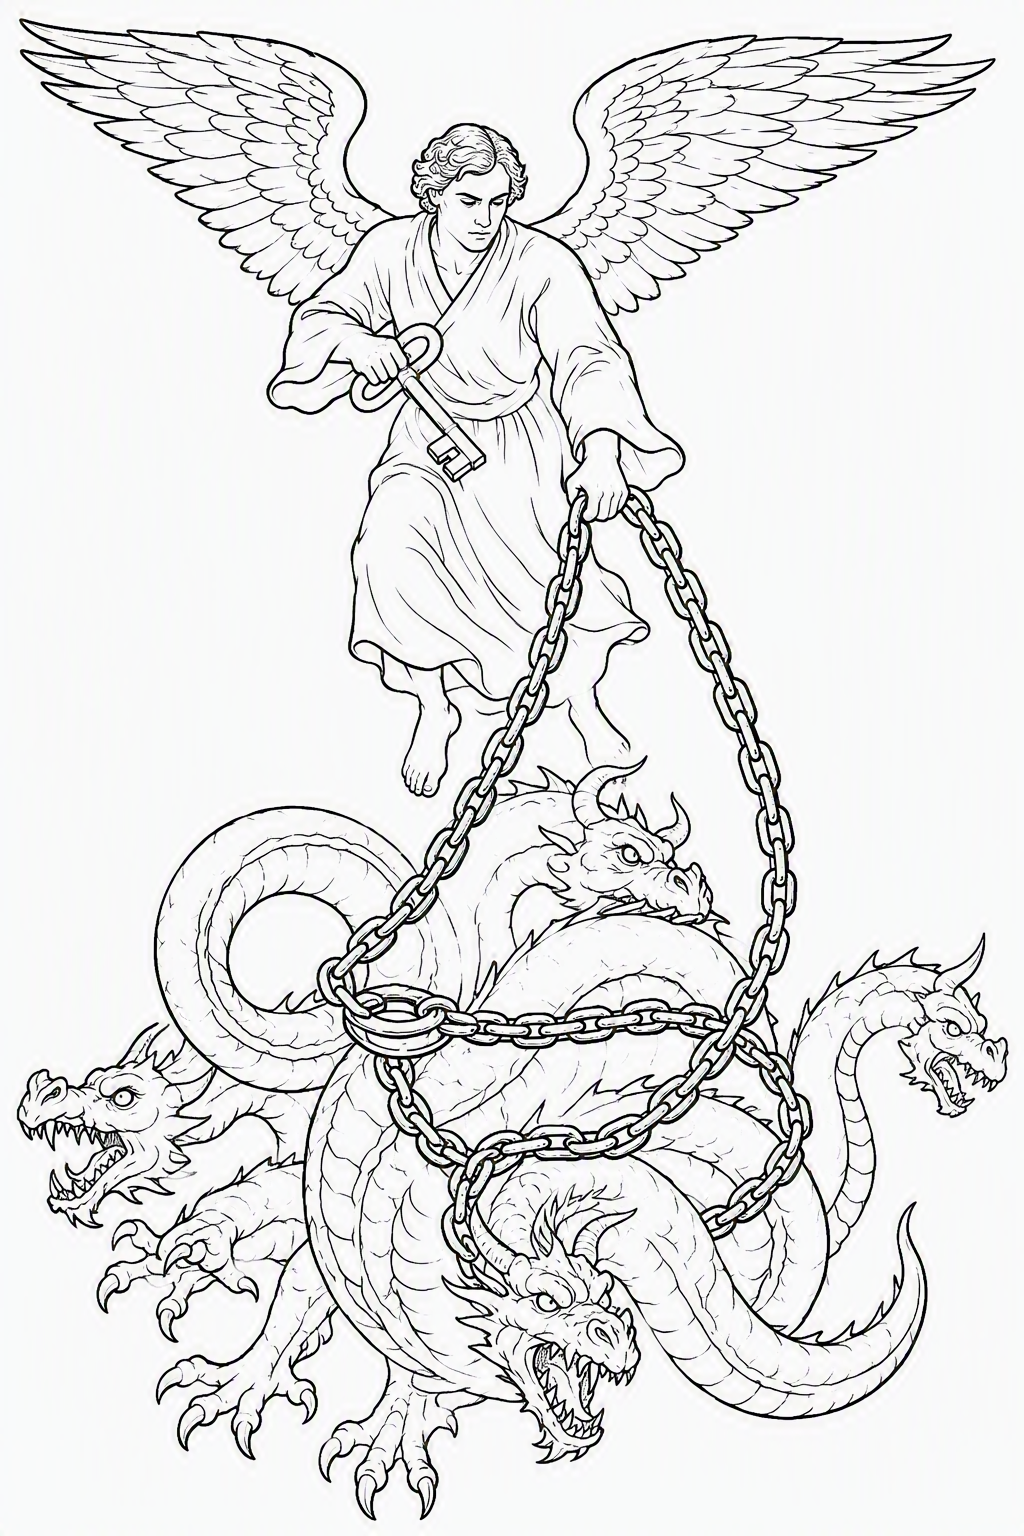
\includegraphics[
    width=0.6\textwidth, 
    trim=0 0 0 0, 
    clip]{images/rev20-satan-bound.png}
    %\caption{}
    %\label{}
\end{figure}




\begin{ScriptureBox}



\item[20:1] 我又看見一位天使從天降下、手裡拿著無底坑的鑰匙、和一條大鍊子。

\item[20:2] 他捉住那龍、就是古蛇、又叫魔鬼、也叫撒但、把他捆綁一千年、

\item[20:3] 扔在無底坑裡、將無底坑關閉、用印封上、使他不得再迷惑列國、等到那一千年完了．以後必須暫時釋放他。

\item[20:4] 我又看見幾個寶座、也有坐在上面的、並有審判的權柄賜給他們．我又看見那些因為給耶穌作見證、並為　神之道被斬者的靈魂、和那沒有拜過獸與獸像、也沒有在額上和手上受過他印記之人的靈魂．他們都復活了、與基督一同作王一千年。

\item[20:5] 這是頭一次的復活。其餘的死人還沒有復活、直等那一千年完了。

\item[20:6] 在頭一次復活有分的、有福了、聖潔了．第二次的死在他們身上沒有權柄．他們必作　神和基督的祭司、並要與基督一同作王一千年。

\item[20:7] 那一千年完了、撒但必從監牢裡被釋放、

\end{ScriptureBox}

讀了以上的經文，我們知道撒但雖然仍然存在，卻被神綑綁，不能迷惑列國。那些忠心跟隨基督的人，會與基督一同作王。

然而你可能就問，為什麼不是「立刻」消滅撒但，而是先捆綁？%
這個問題不是小問題，歷史上從教父時代到如今，就已經多所討論。所以我們也花一點時間了解一下。

\subsection{為什麼不是「立刻」消滅撒但？}

早期教父如游斯丁（Justin Martyr）和愛任紐（Irenaeus），大多理解「捆綁」是將來某一天會發生，基督在大患難之後再度降臨，捆綁撒但，並在地上作王一千年。這可稱為「前千禧年」的解釋。「前」，是基督再臨在千禧年之前。

到了奧古斯丁（Augustine），解釋出現重要轉變。他在《上帝之城》中敘述，撒但已經被捆綁。這「一千年」是「從基督降臨直到末日的教會時代。」這種捆綁並不是說撒但完全不能活動，而是神限制牠「迷惑列國」的能力，使福音得以向列國傳開。中世紀西方教會大體延續奧古斯丁的理解，將「一千年」視為教會時代；撒但仍然可以試探、攻擊人，但牠的權勢受到神的限制，直到末日才接受最終審判。這可稱為「無千禧年」的解釋。

到了近代，前千禧年派受到許多的重視。


\subsection{誰是地上的居民？}

既然復活的聖徒與基督一同作王管理，你可能會問誰是地上的居民？千禧年中可以區分為兩類人：
\begin{itemize}
\item 復活的聖徒：有榮耀、不朽壞的身體。與基督一同作王。
\item 肉身居民：仍然是必死的身體。活在基督的統治之下，並生養後代。
\end{itemize}


\subsection{千禧年}

對這一千年的解釋，可以有前千禧年派，後千禧年派，和無千禧年派等觀點。我特別製表於「附錄：千禧年觀」。我在這裡先列出前千禧年派的解釋。前千禧年派認為，基督會在千禧年之前親自再來，捆綁撒但，使殉道的聖徒復活，並在地上與他們一同作王一千年，之後撒但被釋放、發動最後的叛亂，隨即被永遠扔在火湖裡。

無論是前千禧年派，後千禧年派，或是無千禧年，啟示錄二十章最終都指向同一個高潮：撒但被擊敗，基督的國度進入終極的榮耀。

\section{最後的戰役：歌革與瑪各（Gog Magog）}

\begin{figure}[htbp]
    \centering
    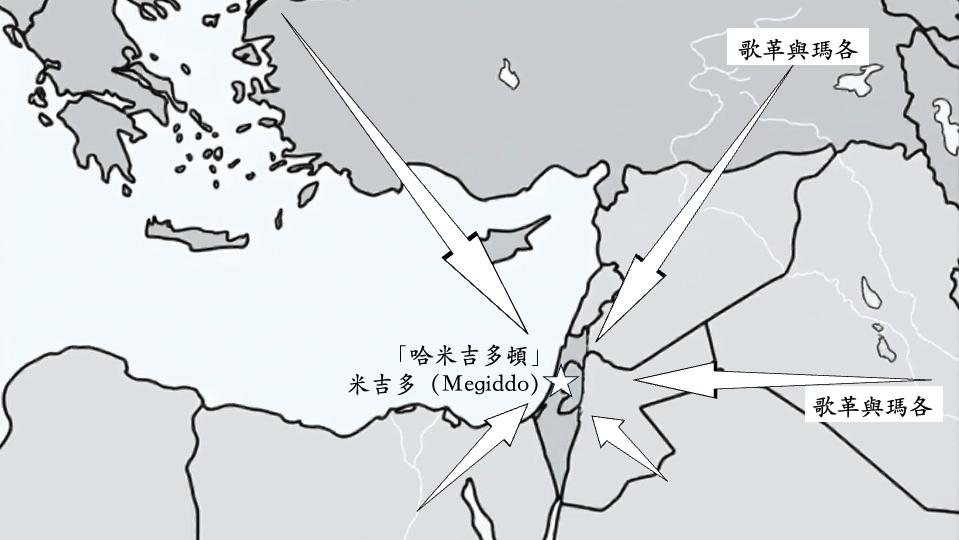
\includegraphics[
    width=1\textwidth, 
    trim=0 0 0 0, 
    clip]{images/armageddon.png}
    %\caption{}
    %\label{}
\end{figure}



\begin{ScriptureBox}

\item[20:8] 出來要迷惑地上四方的列國、〔方原文作角〕就是歌革和瑪各、叫他們聚集爭戰．他們的人數多如海沙。

\item[20:9] 他們上來遍滿了全地、圍住聖徒的營、與蒙愛的城．就有火從天降下、燒滅了他們。

\item[20:10] 那迷惑他們的魔鬼、被扔在硫磺的火湖裡、就是獸和假先知所在的地方．他們必晝夜受痛苦、直到永永遠遠。

\end{ScriptureBox}




歌革與瑪各雖然只在啟示錄20章出現一節經文，但這兩個名稱早已出現在以西結書38至39章。以西結所描述的歌革，是從「北方極處」而來，率領眾多列國攻擊神的子民；到了啟示錄，歌革與瑪各則被描述為從「地的四方」聚集而來，圍住「蒙愛的城」。然而，當敵軍聚集之後，「就有火從天降下來，燒滅了他們」（啟示錄20:9）。

啟示錄在這裡採用了稍微不同的視角，來描述以西結書已經描述的這場末世戰役。
這是神學上的「末世論的重構」（Eschatological reconfiguration）：啟示錄不是單純重複舊約的末世預言，而是將舊約既有的末世意象重新組合、重新定位，使它們在基督的救贖與末世審判的框架中產生新的功能。

值得注意的是，在啟示錄19章，基督已經擊潰在哈米吉多頓集結的敵對勢力，此處20章的歌革與瑪各，則從另一個角度再次描寫此
邪惡勢力的覆滅。
哈米吉多頓與歌革、瑪各都顯示著，邪惡雖然可以在歷史中最後一次聚集，牠的結局已定。

\section{最後的審判：白色大寶座前的終極審判}

\begin{ScriptureBox}

\item[20:11] 我又看見一個白色的大寶座、與坐在上面的．從他面前天地都逃避、再無可見之處了。

\item[20:12] 我又看見死了的人、無論大小、都站在寶座前．案卷展開了．並且另有一卷展開、就是生命冊．死了的人都憑著這些案卷所記載的、照他們所行的受審判。

\item[20:13] 於是海交出其中的死人．死亡和陰間也交出其中的死人．他們都照各人所行的受審判。

\item[20:14] 死亡和陰間也被扔在火湖裡．這火湖就是第二次的死。

\item[20:15] 若有人名字沒記在生命冊上、他就被扔在火湖裡。

\end{ScriptureBox}

約翰看見一個「白色的大寶座」，在祂面前，天地都逃避，再無可見之處。現今的天地將要過去，神的終極審判已經來到。死了的人，無論大小，都站在寶座前，案卷展開，另有一卷就是生命冊。眾人都要按照案卷所記載的，照各人所行的受審判。沒有人能逃避這最後的審判。每一個人都要站在神的審判台前，而最後的結局只有生命與第二次的死兩種。

\begin{figure}[htbp]
    \centering
    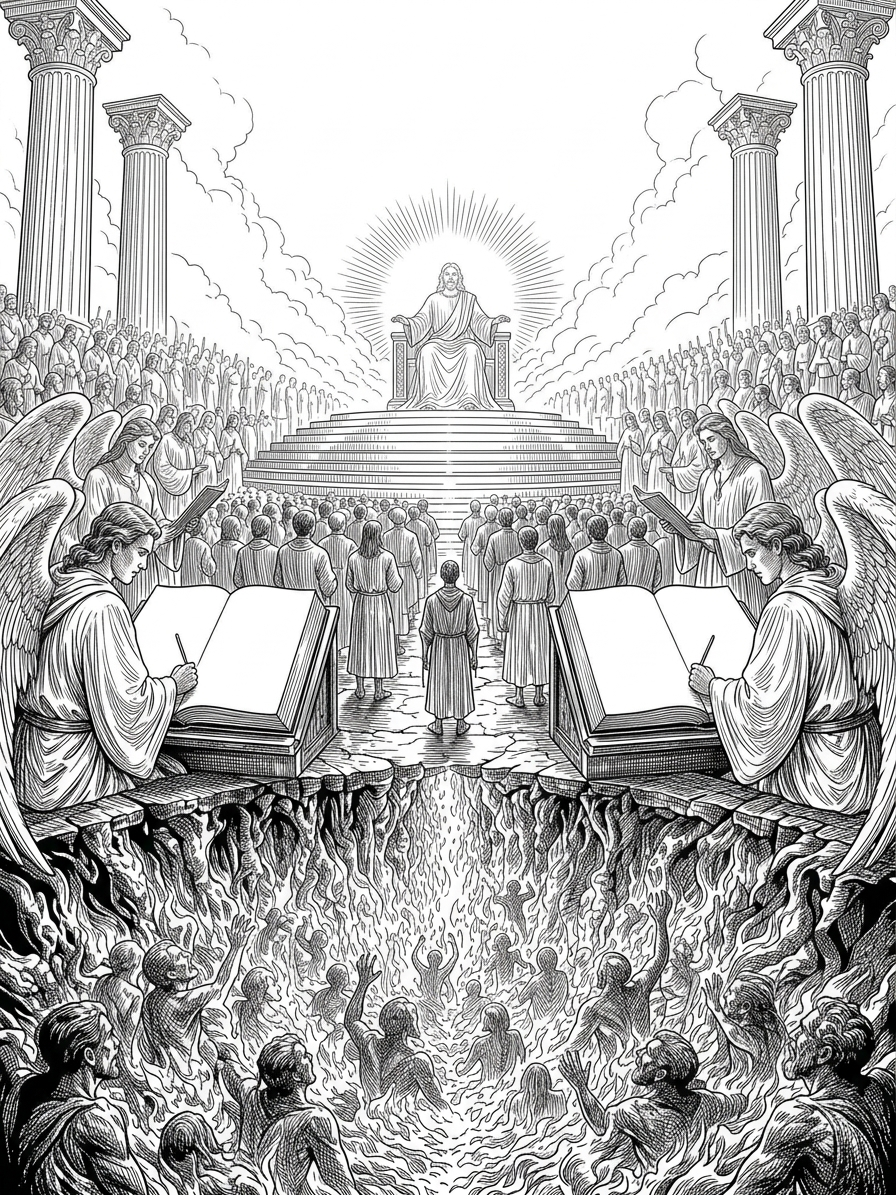
\includegraphics[
    width=1\textwidth, 
    trim=0 0 0 0, 
    clip]{images/white_throne_judgement.jpg}
    %\caption{}
    %\label{}
\end{figure}

\section*{小組討論題}

\begin{enumerate}
    
    \item 讀20:11-15的白色大寶座。這段經文帶給你最大的感受是警醒、敬畏、安慰，還是盼望？為什麼？

    \item 如果你確信基督最終必得勝、撒但必被擊敗、死亡必被除去，你今天的生活會有什麼不同？在家庭、工作、教會或苦難中，你最需要持守的是什麼？
\end{enumerate}

\chapter{被恩典帶入榮耀（21:1-22:21）}

我們終於來到新天新地\idx{13}{新天新地}了。有人可能會問：「我連今生都還沒有走完，為什麼現在就要盼望永生裡的新天新地呢？」

讓我打一個簡單的比方。假設你準備搬進一個寬敞、美麗的新家。新家已經預備好了，你也知道將來要住在那裡。可是家中的孩子和青少年，卻捨不得離開現在熟悉的房子。他們可能會說：「我住在這裡不是很好嗎？為什麼一定要搬走？」你會不會因此告訴他：「既然如此，就不要搬家了。」當然不會。你反而會帶他去看看新家，讓他知道將來要住的是怎樣的地方；你甚至會和他一起期待搬家的那一天。

希伯來書11:16說我們在地上「是客旅、是寄居的。」而我們是要「羨慕一個更美的家鄉、就是在天上的，」並且「神已經給他們預備了一座城。」主耶穌要離世的時候，也告訴我們「我去是為你們預備地方。」（約翰福音14:2）我們對新天新地的盼望也是如此。

我們並不是因為厭惡今生，才盼望將來。相反地，我們是在今生經歷神的恩典\idx{10}{恩典}、認識基督、愛人、服事主。但我們知道，這一切仍不是故事的終點。
神已經為祂的子民預備了一個更美的家鄉。那是神最終更新天地、與祂的子民永遠同住的榮耀\idx{14}{榮耀}居所。
所以，基督徒可以一面珍惜今天，一面期待那一天；一面忠心走完今生的道路，一面抬頭仰望將來的榮耀。


\begin{figure}[htbp]
    \centering
    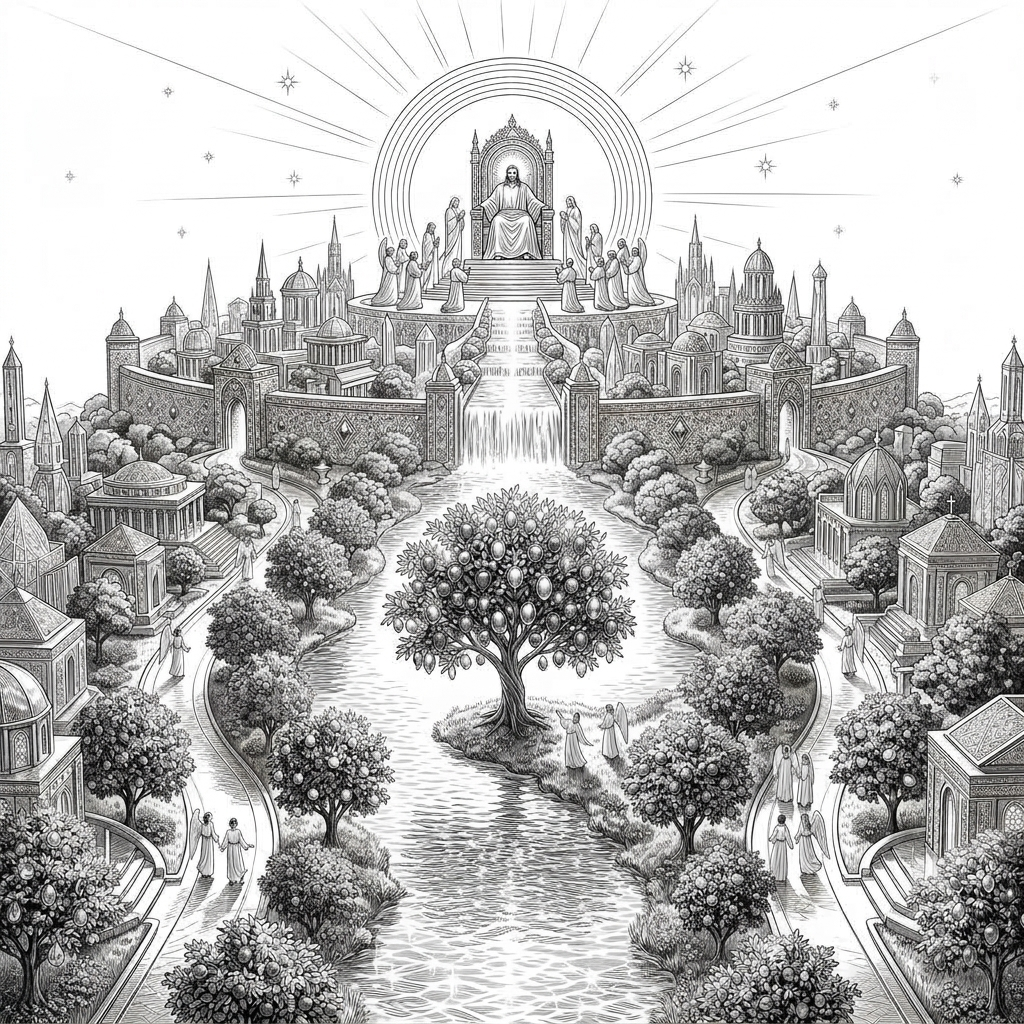
\includegraphics[
    width=1\textwidth, 
    trim=0 0 0 0, 
    clip]{images/tree_of_life.jpg}
\end{figure}



\section{一切更新，神與人同住}

\begin{ScriptureBox2}{圈出21:1–4中一切「不再有」的事物。坐寶座的說祂要將什麼更新？祂要白白賜給口渴的人什麼？}

\item[21:1]
\textit{我又看見一個新天新地．因為先前的天地已經過去了．海也不再有了。}

\item[21:2]
\textit{我又看見聖城新耶路撒冷由　神那裡從天而降、預備好了、就如新婦妝飾整齊、等候丈夫。}

\item[21:3]
\textit{我聽見有大聲音從寶座出來說、看哪、　神的帳幕在人間．他要與人同住、他們要作他的子民、　神要親自與他們同在、作他們的　神．}

\item[21:4]
\textit{神要擦去他們一切的眼淚．不再有死亡、也不再有悲哀、哭號、疼痛、因為以前的事都過去了。}

\item[21:5]
\textit{坐寶座的說、看哪、我將一切都更新了。又說、你要寫上．因這些話是可信的、是真實的。}

\item[21:6]
\textit{他又對我說、都成了。我是阿拉法、我是俄梅戛、我是初、我是終。我要將生命泉的水白白賜給那口渴的人喝。}

\item[21:7]
\textit{得勝的、必承受這些為業．我要作他的　神、他要作我的兒子。}

\item[21:8]
\textit{惟有膽怯的、不信的、可憎的、殺人的、淫亂的、行邪術的、拜偶像的、和一切說謊話的、他們的分就在燒著硫磺的火湖裡．這是第二次的死。}

\end{ScriptureBox2}

我們看到的一個重要的字，是「新天新地\idx{13}{新天新地}」、「新耶路撒冷\idx{13}{新耶路撒冷}」裡的「新」。這個「新」究竟是什麼意思？如果我們還是原來的「舊人」，帶著舊的生命、舊的性情、舊的罪進入新天新地，豈不是很不相稱嗎？所以，神不只是更新天地，也要把祂的子民生命中更新，使我們成為與祂永遠同住的人。保羅說：「所以我們不喪膽。外體雖然毀壞，內心卻一天新似一天。」（哥林多後書4:16）我們不是到了新天新地才開始更新，而是今天就已經在基督裡經歷更新；到了那一天，神要把這更新帶到完全。

我們可以想到十字架上的那個強盜。他原本是罪犯，與耶穌一同被釘十字架。然而，就在生命最後的時刻，他看見了與他同釘的耶穌，承認自己的罪，並求主記念他。耶穌對他說：「今日你要同我在樂園裡了。」（路加福音23:43）這個人沒有時間重新建立自己的人生，也沒有機會靠自己的行為證明自己已經改變；但他的心轉向了基督。他從一個犯罪的人，成為一個仰望基督、信靠基督的人。這就是恩典\idx{10}{恩典}所帶來的更新。所以，新天新地所迎接的，不是一群仍然愛慕罪惡的「舊人」，而是神已經在基督裡更新、如今仍在被祂更新，並且將來要完全得榮耀\idx{14}{榮耀}的子民。

更新一切的是誰呢？祂說「成了」。祂說「我是阿拉法、我是俄梅戛、我是初、我是終。」祂是「將生命泉的水白白賜給那口渴的人喝。」祂是在約翰福音4:14 雅各井邊，對那位婦人說「人若喝我所賜的水就永遠不渴．我所賜的水、要在他裡頭成為泉源、直湧到永生。」

\section{新婦就是新耶路撒冷}

\begin{ScriptureBox2}{數一數21:12–21中所有的「十二」。門上寫著誰的名字？根基上又寫著誰的名字？}

\item[21:9]
\textit{拿著七個金碗、盛滿末後七災的七位天使中、有一位來對我說、你到這裡來、我要將新婦、就是羔羊的妻、指給你看。}

\item[21:10]
\textit{我被聖靈感動、天使就帶我到一座高大的山將那由　神那裡從天而降的聖城耶路撒冷指示我。}

\item[21:11]
\textit{城中有　神的榮耀．城的光輝如同極貴的寶石、好像碧玉、明如水晶．}

\item[21:12]
\textit{有高大的牆．有十二個門、門上有十二位天使．門上又寫著以色列十二個支派的名字．}

\item[21:13]
\textit{東邊有三門．北邊有三門．南邊有三門．西邊有三門。}

\item[21:14]
\textit{城牆有十二根基、根基上有羔羊十二使徒的名字。}

\item[21:15]
\textit{對我說話的拿著金葦子當尺、要量那城、和城門城牆。}

\item[21:16]
\textit{城是四方的、長寬一樣、天使用葦子量那城、共有四千里．長寬高都是一樣。}

\item[21:17]
\textit{又量了城牆、按著人的尺寸、就是天使的尺寸、共有一百四十四肘。}

\item[21:18]
\textit{牆是碧玉造的．城是精金的、如同明淨的玻璃。}

\item[21:19]
\textit{城牆的根基是用各樣寶石修飾的。第一根基是碧玉．第二是藍寶石．第三是綠瑪瑙．第四是綠寶石．}

\item[21:20]
\textit{第五是紅瑪瑙．第六是紅寶石．第七是黃璧璽．第八是水蒼玉．第九是紅璧璽．第十是翡翠．第十一是紫瑪瑙．第十二是紫晶。}

\item[21:21]
\textit{十二個門是十二顆珍珠．每門是一顆珍珠．城內的街道是精金、好像明透的玻璃。}

\end{ScriptureBox2}


聖城\idx{13}{聖城}由天而降，充滿光輝，大有榮耀\idx{14}{榮耀}。約翰仔細觀看。每一面有三個門，寫了以色列\idx{05}{以色列}十二個支派的名字．約翰看的非常仔細。城牆有十二根基、根基上有羔羊\idx{10}{羔羊}十二使徒的名字。這不禁使我們想起，耶穌對彼得說：「你是彼得，我要把我的教會建造在這磐石上；陰間\idx{11}{陰間}的權柄不能勝過他。」（馬太福音16:18）。聖城新耶路撒冷\idx{13}{新耶路撒冷}不僅有十二根基（代表新約的十二使徒），還有十二個門（上面寫著以色列十二個支派的名字）。這表明上帝救贖\idx{11}{救贖}計畫是完整的，將舊約的以色列選民與新約的基督教會，完美地結合在同一個榮耀的居所中。這段經文提醒著所有基督徒，教會的信仰是有根有基的，正是建立在使徒和先知的根基上，並且以耶穌基督自己為房角石（以弗所書 2:20）。

\begin{InDepth}
\InDepthHeading{新耶路撒冷有多大？}

這裡特別給了城的尺寸，那是象徵完全、聖潔、無缺。這城是一個正立方體，長、寬、高都相等約有「四千里」。
以現代的尺寸來換算，約1,400 英里。\footnotemark

\begin{center}
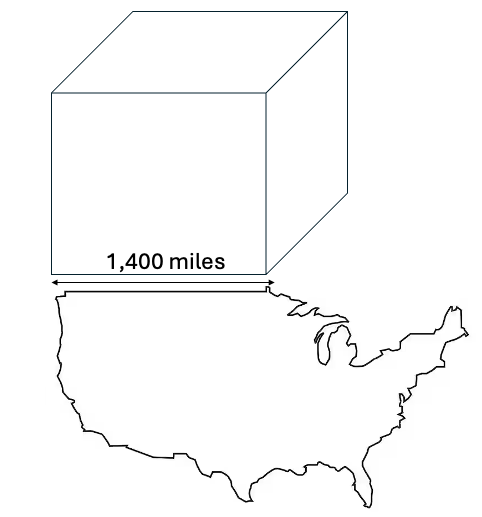
\includegraphics[width=0.6\linewidth]{images/new_jesusalem_US.png}
\end{center}

美國東西方向寬度的一半約1,400 英里。現在，
請想像這樣一座巨大的立方體。長、寬、高是1,400 英里。
那個燦爛浩大的城。
\end{InDepth}
% Footnote text for the mark in the box above
\footnotetext{希臘文原文是一萬二千 stadia。和合本中文聖經翻譯者採用了一個換算：3 stadia ≈ 1 里。12,000 stadia ÷ 3 = 4,000 里。所以才有「共有四千里」。}

並且，
啟示錄7:9告訴我們那站在寶座\idx{20}{寶座}和羔羊面前的，是「沒有人能數過來的各國、各族、各民、各方」的群眾。
是所有在永生中的人可以自由行走的。

這個簡單的比較，只是幫助我們稍微想像聖城的宏偉與廣大。當我們思想這樣的尺度時，可以驚嘆神的創造何等浩大、祂為祂子民所預備的榮耀何等超越我們的想像。
正如保羅所說：「神為愛他的人所預備的是眼睛未曾看見，耳朵未曾聽見，人心也未曾想到的。」（哥林多前書2:9）




\section{神自己就是城的殿}

\begin{ScriptureBox2}{約翰在城內沒有看見什麼？為什麼？城的光從哪裡來？誰才得進那城？}

\item[21:22]
\textit{我未見城內有殿、因主　神全能者、和羔羊、為城的殿。}

\item[21:23]
\textit{那城內又不用日月光照．因有　神的榮耀光照．又有羔羊為城的燈。}

\item[21:24]
\textit{列國要在城的光裡行走．地上的君王必將自己的榮耀歸與那城。}

\item[21:25]
\textit{城門白晝總不關閉．在那裡原沒有黑夜。}

\item[21:26]
\textit{人必將列國的榮耀尊貴歸與那城。}

\item[21:27]
\textit{凡不潔淨的、並那行可憎與虛謊之事的、總不得進那城．只有名字寫在羔羊生命冊上的纔得進去。}

\end{ScriptureBox2}

在城中的人，是蒙恩得救的人；他們的名字已經寫在羔羊\idx{10}{羔羊}生命冊\idx{05}{生命冊}上。 他們是神恩典\idx{10}{恩典}的工作。祂在基督裡揀選、呼召、赦免並保守祂的子民，最終把他們帶進這座永恆的城。因此，新天新地\idx{13}{新天新地}中的人既有共同的身分，都是羔羊所救贖\idx{11}{救贖}的子民；又保留各族的豐富與多樣。差異不再成為分裂的原因，反而成為共同榮耀\idx{14}{榮耀}神的豐富色彩。這是一個何等美麗的畫面！

\begin{ReaderQuestion}
從伊甸園、會幕、聖殿、基督道成肉身，一直到新天新地，你看見神與人同住的應許如何逐步展開？
\end{ReaderQuestion}

\section{生命的河與生命樹}

\begin{ScriptureBox2}{生命水的河從哪裡流出來？劃出22:3–5中神的僕人要做的事和要看見的。}

\item[22:1]
\textit{天使又指示我在城內街道當中一道生命水的河、明亮如水晶、從　神和羔羊的寶座流出來。}

\item[22:2]
\textit{在河這邊與那邊有生命樹、結十二樣果子、〔樣或作回〕每月都結果子．樹上的葉子乃為醫治萬民。}

\item[22:3]
\textit{以後再沒有咒詛．在城裡有　神和羔羊的寶座．他的僕人都要事奉他．}

\item[22:4]
\textit{也要見他的面．他的名字必寫在他們的額上。}

\item[22:5]
\textit{不再有黑夜．他們也不用燈光日光．因為主　神要光照他們．他們要作王、直到永永遠遠。}

\end{ScriptureBox2}

22:1–2首先把讀者帶回《創世記》的伊甸園\idx{06}{伊甸園}。在伊甸園中有生命樹\idx{05}{生命樹}，也有河流。生命水\idx{05}{生命水}的河是「從神和羔羊\idx{10}{羔羊}的寶座\idx{20}{寶座}流出來。」人的生命倚靠神並享受神的福樂，是受造的恩典\idx{10}{恩典}。這裡的生命樹「每月都結果子」，持續供應人的生命，使人永遠豐盛。

「樹上的葉子乃為醫治萬民」並不是說新創造中還存在疾病。這個果子吃了使人愉悅，比較像是超級維他命的概念。吃了的人精神百倍，心裡暢快。\footnote{MacArthur, J. (2007).}

\begin{InDepth}
\InDepthHeading{失樂園與復樂園}

22:3說：「以後再沒有咒詛」，使我們想到創世記3章，罪進入世界，咒詛隨之而來；啟示錄22章，救贖\idx{11}{救贖}完成，咒詛被徹底除去。如果我們比較兩者，我們可以得到非常好的理解：

\par\medskip\noindent
\begin{minipage}{\linewidth}
\centering\small
\renewcommand{\arraystretch}{1}\setlength{\tabcolsep}{4pt}
\captionof{table}{創世記3章與啟示錄21--22章}
\label{tab:genesis3-rev21-22-zh}
\begin{tabularx}{\linewidth}{>{\raggedright\arraybackslash}X
                              >{\raggedright\arraybackslash}X}
\hline
創世記3章 & 啟示錄21--22章 \\
\hline
罪進入世界 & 一切都更新 \\
咒詛臨到 & 不再有咒詛 \\
被趕出伊甸園 & 進入聖城\idx{13}{聖城} \\
不能吃生命樹 & 得著生命樹 \\
與神隔絕 & 神與人同住 \\
死亡進入世界 & 不再有死亡 \\
蛇引誘人 & 撒但\idx{15}{撒但}完全敗亡 \\
人失去神的面 & 「也要見他的面」 \\
\hline
\end{tabularx}
\end{minipage}
\end{InDepth}


\section{這書不可封閉}

\begin{ScriptureBox2}{在這段經文中，耶穌說了幾次「我必快來」？圈出每一個「有福了」，並留意誰是有福的。}

\item[22:6]
\textit{天使又對我說、這些話是真實可信的．主就是眾先知被感之靈的　神、差遣他的使者、將那必要快成的事指示他僕人。}

\item[22:7]
\textit{看哪、我必快來。凡遵守這書上預言的有福了。}

\item[22:8]
\textit{這些事是我約翰所聽見所看見的．我既聽見看見了、就在指示我的天使腳前俯伏要拜他。}

\item[22:9]
\textit{他對我說、千萬不可．我與你、和你的弟兄眾先知、並那些守這書上言語的人、同是作僕人的．你要敬拜　神。}

\item[22:10]
\textit{他又對我說、不可封了這書上的預言．因為日期近了。}

\item[22:11]
\textit{不義的、叫他仍舊不義．污穢的、叫他仍舊污穢．為義的、叫他仍舊為義．聖潔的、叫他仍舊聖潔。}

\item[22:12]
\textit{看哪、我必快來．賞罰在我、要照各人所行的報應他。}

\item[22:13]
\textit{我是阿拉法、我是俄梅戛、我是首先的、我是末後的、我是初、我是終。}

\item[22:14]
\textit{那些洗淨自己衣服的有福了、可得權柄能到生命樹那裡、也能從門進城。}

\item[22:15]
\textit{城外有那些犬類、行邪術的、淫亂的、殺人的、拜偶像的、並一切喜好說謊言編造虛謊的。}

\end{ScriptureBox2}

現在，啟示錄是直接對你我勸勉。天使宣告：「這些話是真實可信的。」因為這卷書是要讓神的百姓公開宣讀、聽見遵守而得福的。

這裡，我們又一次聽見耶穌宣告祂自己的身分：「我是阿拉法，我是俄梅戛，我是首先的，我是末後的，我是初，我是終。」阿拉法（Alpha）是希臘文的第一個字母，俄梅戛（Omega）是最後一個字母。整個世界的歷史都在祂的掌權之下。從創世直到新天新地\idx{13}{新天新地}，從十字架到榮耀\idx{14}{榮耀}，沒有任何事情超出祂的計畫。

「不義的，叫他仍舊不義……聖潔的，叫他仍舊聖潔。」這句話的意思是說，義人與惡人個別的心思意念完全顯露付諸行動。人的生命所結出的果子，最終顯明他是否屬於羔羊\idx{10}{羔羊}。人在今生所持守的道路，將在永恆中顯明其最終的歸屬。

\section{最後的福音邀請：口渴的人都可以來}

\begin{ScriptureBox2}{耶穌在22:16如何描述自己？誰說「來」？誰被邀請取生命的水喝？}

\item[22:16]
\textit{我耶穌差遣我的使者為眾教會將這些事向你們證明。我是大衛的根、又是他的後裔．我是明亮的晨星。}

\item[22:17]
\textit{聖靈和新婦都說來。聽見的人也該說來。口渴的人也當來．願意的都可以白白取生命的水喝。}

\end{ScriptureBox2}


最後，啟示錄再提出邀請，是向每一個讀到這卷書、仍然「口渴」的人發出最美好的福音呼召：「口渴的人也當來；願意的，都可以白白取生命的水喝。」（啟 22:17）這讓我們想起主耶穌在井旁對撒瑪利亞婦人所說的話：「人若喝我所賜的水就永遠不渴。我所賜的水，要在他裡頭成為泉源，直湧到永生。」（約 4:14）神希望將人帶到祂永生的榮耀\idx{14}{榮耀}裡，飲用祂賜給人的生命水\idx{05}{生命水}，直到永生。

\begin{ReaderQuestion}
如果你要向一位尚未信主、但正在人生中感到「口渴」的人解釋這句話，你會怎樣說？這節經文如何顯明福音是恩典，而不是靠人的功德換取？
\end{ReaderQuestion}

\section{「主耶穌啊，我願你來」}

\begin{ScriptureBox2}{關於這書上的預言，有什麼警告？教會在22:20如何回應耶穌的應許？}

\item[22:18]
\textit{我向一切聽見這書上預言的作見證、若有人在這預言上加添甚麼、　神必將寫在這書上的災禍加在他身上．}

\item[22:19]
\textit{這書上的預言、若有人刪去甚麼、　神必從這書上所寫的生命樹、和聖城、刪去他的分。}

\item[22:20]
\textit{證明這事的說、是了．我必快來。阿們。主耶穌阿、我願你來。}

\item[22:21]
\textit{願主耶穌的恩惠、常與眾聖徒同在。阿們。}

\end{ScriptureBox2}


書的結語是主耶穌的「我必快來」，以及人的回應「我願你來」。使我們想起《雅歌》中良人與女子彼此渴望的對話。新婦\idx{13}{新婦}所盼望的，不只是婚宴本身，而是良人親自來到。同樣，教會所等候的，是那位愛我們、為我們捨己、又從死裡復活的羔羊\idx{10}{羔羊}親自來到。我們何其有幸，可以與主對話，祂的「我必快來」，是我的持守，是我在患難中的力量。

\begin{ReaderQuestion}
對你而言，「主耶穌啊，我願你來」不只是對未來的盼望，也可以如何成為今天生活的禱告？在工作、家庭、苦難、服事和面對不確定的未來時，這個盼望可以怎樣改變我們？
\end{ReaderQuestion}

%\chapter*{附錄：常見的問題}
%\addcontentsline{toc}{chapter}{附錄：常見的問題}

\appendix
\renewcommand{\appendixname}{附錄}
\renewcommand{\thechapter}{\arabic{chapter}}
\renewcommand{\thefigure}{\appendixname~\thechapter.\arabic{figure}}  % Appendix 1.1, 1.2, …

\refstepcounter{chapter}
\chapter*{附錄：常見的問題}
\addtocontents{toc}{\protect\setlength{\cftbeforechapskip}{0.3em}}
\addcontentsline{toc}{chapter}%
  {\appendixname~\thechapter\quad 常見的問題}



\section*{當你深愛的弟兄（或是姐妹）離世了，可是你走不出傷痛。}

你必定很深地想念那位與你一同走過生命的弟兄或是姐妹，也很深地渴望天家。我想，主知道你心裡的思念，也知道這段離別的路有多麼不容易。但今天，主仍然把你留在世上。你不是被留下來獨自承受痛苦，而是被主的恩典追上的人，將來還要被主的恩典帶入榮耀裡。

有一天，我們要與天地的主宰基督同在。而我們最大的盼望，就是永遠與主同在，親眼見祂的榮耀。在祂裡面，我們也有與所有屬主的人一同進入永恆的盼望。

願姊妹在思念弟兄的日子裡，仍然仰望基督。祂不僅是我們今生的倚靠，也是我們永恆的盼望。願主親自扶持你，使你在每一天的生活中，都能經歷祂的同在與恩典。
主給我們的應許，是祂要擦去我們的眼淚。

傳道書 3:1、4 告訴我們，凡事都有定期，哭有時，笑有時；哀慟有時，跳舞有時。
如果你開始快樂，不是代表沒有那麼愛他了。如果你去旅行、或參加聚會，也不是代表你已經忘記了他了。
你可以繼續珍惜與先生共同生活的回憶，也可以慢慢學習適應沒有先生陪伴的日子。


\section*{當復活的時候，人也不娶也不嫁，乃像天上的使者一樣（馬太福音 22:30）}

我只能想像啟示錄 7:9--10 所描繪的那個場景：
「有許多的人，沒有人能數過來，是從各國各族各民各方來的，站在寶座和羔羊面前，身穿白衣，手拿棕樹枝，大聲喊著說：『願救恩歸與坐在寶座上我們的神，也歸與羔羊。』」

也許，在那壯闊的隊伍中，你看見了自己的配偶。
可是，你眼前的他，已經不再是你在地上所熟悉的模樣。他身穿白衣，眼中有光，正興奮地讚美救恩的偉大。他全心全意地敬拜那位救贖他的主。此刻，他的生命完全以基督為中心；他所渴慕的，是在永生裡親近主、認識主、讚美主，與主同行。

你也許會發現，將來的他，遠超過你今生所認識的他。
你從前很了解這位弟兄。你知道他的事業曾經是他生活中的重心，也知道他每天上班前習慣喝一杯咖啡。你熟悉他的習慣、他的喜怒哀樂，也陪伴他走過人生的高低起伏。然而，到了那日，他將不再受今世的軟弱、勞苦與憂愁所限制，而是得著不朽壞、榮耀的身體（哥林多前書 15:42--44）。

可是，你也變了。
你同樣站在那群從各國各族各民各方而來的人中間，身穿白衣，手拿棕樹枝，向坐在寶座上的神和羔羊獻上讚美。那位最完全地認識你、最深地愛你，也為你捨命的救主，如今就在你面前。你將以全新的生命愛祂、敬拜祂，在永恆中與祂同行。

哥林多前書 13:12 說：「我們如今彷彿對著鏡子觀看，模糊不清……到那時就要面對面了。」我們今天對主的認識仍然有限，但將來要更完全地認識祂。到了那日，我們不再只是憑著信心仰望主，而是要親自見到祂。我們將與眾聖徒一同站在羔羊面前，敬拜那位為我們捨命、救贖我們的主，永遠享受祂的同在。



\section*{如果將來我在天國，所愛的家人卻不在那裡，我還能快樂嗎？}

當我們想到自己的父母、配偶、兒女或兄弟姊妹，如果有一天我們在天國，而所愛的人卻不在那裡，我們怎麼可能不感到悲傷呢？

我們也許會問：到了永恆裡，我們是否仍然記得今生所愛的人？如果記得，我們是否仍然愛他們？如果愛仍然存在，而他們卻沒有得救，我們又怎麼可能在沒有悲傷的情況下享受永恆？

聖經確實啟示了永恆的盼望、神的公義，以及祂要除去一切悲哀的應許；但聖經並沒有完整解釋，得救者在新天新地中將如何經歷對失喪親人的記憶與感情。因此，我們需要謙卑承認，聖經沒有明確說明的部分，不應被我們的推測取代。

第一點，到了天國，我們是否還會記得不信主的家人？我們知道耶穌復活以後，祂仍然是那位被釘十字架、後來復活的主。神也會改變形狀我們這卑賤的身體，使我們和他自己榮耀的身體相似。（腓立比書3:21）

第二點：如果仍然記得，看到所愛的人不在天國，怎麼可能快樂？
假設一位母親在天國，卻知道自己的兒子沒有得救；或者一位丈夫在神的同在中，卻知道自己所愛的妻子沒有進入永恆的生命。我們很難想像，他怎麼可能完全沒有悲傷。

如果愛仍然存在，失去所愛之人的痛苦怎麼可能消失？
啟示錄21:4應許我們：
「神要擦去他們一切的眼淚；不再有死亡，也不再有悲哀、哭號、疼痛，因為以前的事都過去了。」
神要親自擦去祂子民一切的眼淚，使死亡、悲哀、哭號與疼痛不再成為他們生命的一部分。

然而，這段經文並沒有詳細說明，神將如何更新我們的記憶、情感與理解，使我們在新天新地中完全享受祂的同在。
我們所能確信的是，神的應許不會落空。

此外，到了永恆，我們將完全承認神的審判是公義的。啟示錄 16:7 宣告：
「主神啊，你的判斷義哉！誠哉！」
祂的判斷完全公義，也完全符合祂自己的聖潔。
然而，承認神的審判完全公義，並不等於我們已經知道，得救者將如何理解或經歷未得救親人的結局。

第三點：神的聖潔與憐憫並不矛盾。
耶穌在地上時，祂知道人的罪，也知道審判的真實，卻仍然為耶路撒冷哀哭。
馬太福音 23:37 記載，耶穌說：
「耶路撒冷啊，耶路撒冷啊……我多次願意聚集你的兒女，好像母雞把小雞聚集在翅膀底下，只是你們不願意。」
這段經文讓我們看見，耶穌的聖潔與祂對人的憐憫並不矛盾。
祂沒有因為知道人的罪，就失去對人的憐憫；祂也沒有因為愛人，就否定神的真理與審判。祂的憐憫是真實的，祂的審判也是公義的。

那麼，今天的我們應當如何面對這個問題？
我們仍然可以關心家人的屬靈生命，為他們禱告，也可以為他們流淚。
保羅曾為以色列同胞深深憂傷，甚至說自己為他們大有憂愁，心裡時常傷痛（羅馬書9:2-3）。
這提醒我們，對所愛之人的得救有深切的負擔，並不表示我們缺乏信心。
今天，我們仍然可以為所愛的人禱告，向他們分享福音，也將自己無法掌握的事交託給神。
%\chapter*{附錄：各種末世論觀點}
%\addcontentsline{toc}{chapter}{附錄：各種末世論觀點}


%\appendix
\renewcommand{\appendixname}{附錄}
\renewcommand{\thechapter}{\arabic{chapter}}
\renewcommand{\thefigure}{\appendixname~\thechapter.\arabic{figure}}  % Appendix 1.1, 1.2, …

\refstepcounter{chapter}
\chapter*{附錄：各種末世論觀點}
\addcontentsline{toc}{chapter}%
  {\appendixname~\thechapter\quad 各種末世論觀點}




啟示錄主要有四種解釋方式。它們最大的分別在於：啟示錄所描述的事，是發生在過去、整段歷史、將來，還是每個時代？

\subsection*{未來派（Futurism）}
未來派的特色是「將來」。它認為第4章以後的異象大多尚未發生，要在基督再來前後按次序實現，例如將來會有一位具體的敵基督、一段大災難時期，以及基督再來後在地上的千年國度。與其他三派相比，未來派最按照字面和時間順序來讀經文：過去派認為這些事已經發生，歷史派認為正在歷史中逐步發生，理想派則不把它們對應到特定事件。未來派的長處是重視預言的應驗，提醒信徒警醒等候主再來；難處是使啟示錄的大部分內容與第一世紀的讀者似乎關係不大。

\subsection*{過去派（Preterism）}
過去派的特色是把啟示錄的重心放在「過去」，即約翰當時的第一世紀。它認為書中的預言大多已經應驗，所指的是羅馬帝國對教會的逼迫，以及主後70年耶路撒冷被毀。與其他三派相比，過去派最重視歷史背景和第一世紀的初代教會。約翰明說這些事「必要快成」（啟示錄1:1），所以它首先是寫給當時受逼迫教會的安慰。它的長處是讓經文與初代教會緊密相連；難處是較難解釋書中描述的全面審判與萬物更新，因此多數過去派仍相信基督將來要再來。

\subsection*{歷史派（Historicism）}
歷史派的特色是把啟示錄看作「一部按次序展開的教會歷史」，從使徒時代一直延伸到基督再來。它不像過去派只看第一世紀，也不像未來派只看未來，而是認為書中的異象對應歷史上一連串具體事件與人物，例如七間教會代表教會歷史的七個時期。宗教改革時期這種讀法最為盛行。它的長處是強調神掌管歷史的每一個階段；難處是各家對應的事件往往不同，而且每一代人都容易把自己的時代當成歷史的高潮，所以今天較少學者採用。

\subsection*{理想派／象徵派（Idealism）}
理想派的特色是不把啟示錄對應到任何「特定」的歷史事件，而是把它讀成描繪「每個時代」都存在的屬靈實況：神與撒但的爭戰、教會受苦作見證、邪惡勢力的引誘，以及基督終必得勝。其他三派都在問「這件事何時發生」，理想派卻問「這段異象揭示了什麼屬靈真理」。它的長處是讓啟示錄對每一代信徒都直接適用；難處是可能忽略書中確實具有的歷史背景與應驗的部分。因此許多學者會把理想派與其他觀點結合，例如先看經文在第一世紀的意義，再看它對歷代教會的啟示，最後指向基督的再來。

四者並非互相排斥：一個異象可以先指向羅馬帝國，同時呈現歷代教會的屬靈爭戰，並指向基督最後的得勝。

%\chapter*{附錄：大災難多久？但以理書的七十個七}
%\phantomsection
%\addcontentsline{toc}{chapter}{附錄：大災難多久？但以理書的七十個七}
%\markboth{附錄：大災難多久？但以理書的七十個七}{附錄：大災難多久？但以理書的七十個七}

%\setcounter{figure}{0}
%\renewcommand{\thefigure}{\arabic{figure}}   % this is the line that fixes \ref
%\def\theHfigure{appendix.\arabic{figure}}




%\appendix
\renewcommand{\appendixname}{附錄}
\renewcommand{\thechapter}{\arabic{chapter}}
\renewcommand{\thefigure}{\appendixname~\thechapter.\arabic{figure}}  % Appendix 1.1, 1.2, …

\refstepcounter{chapter}
\chapter*{附錄：大災難多久？但以理書的七十個七}
\addcontentsline{toc}{chapter}%
  {\appendixname~\thechapter\quad 大災難多久？但以理書的七十個七}





\section*{一般說法：「七年」的大災難}
以下是前千禧年派的觀點。
但以理書9章是理解末後年日的關鍵。
\begin{ScriptureBox}

\item[9:24] 為你本國之民、和你聖城、已經定了七十個七、要止住罪過、除淨罪惡、贖盡罪孽、引進〔或作彰顯〕永義、封住異象和預言、並膏至聖者。〔者或作所〕
\item[9:25] 你當知道、當明白、從出令重新建造耶路撒冷、直到有受膏君的時候、必有七個七、和六十二個七．正在艱難的時候、耶路撒冷城連街帶濠、都必重新建造。
\item[9:26] 過了六十二個七、那受膏者〔那或作有〕必被剪除、一無所有、必有一王的民來毀滅這城、和聖所．至終必如洪水沖沒、必有爭戰．一直到底、荒涼的事已經定了。
\item[9:27] 一七之內、他必與許多人堅定盟約、一七之半、他必使祭祀與供獻止息．那行毀壞可憎的〔或作使地荒涼的〕如飛而來、並且有忿怒傾在那行毀壞的身上、〔或作傾在那荒涼之地〕直到所定的結局。

\end{ScriptureBox}

天使對但以理說，神為以色列民和耶路撒冷「已經定了七十個七」。
這裡的「七」原文是「七的單位」，按上下文指的是「年」，所以70個七就是 $70 \times 7 = 490$ 年。
第70個七，是大災難時期，是七年。

以上的「7個七」（49年）和「62個七」（434年），在歷史上已經應驗。
\begin{itemize}
\item 「7個七」（49年）：一般認為這是指波斯王亞達薛西在位第二十年（約主前445年）給尼希米的命令（尼希米2:1-8）。是從「重新建造耶路撒冷」開始。
\item 「62個七」（434年）：與前一段合計69個七，也就是483年。如果按聖經預言中常用的一年360日計算，483年約為173,880日，正好落在主耶穌騎驢進耶路撒冷、被尊為君王的時候。「那受膏者必被剪除，一無所有」，明確指向基督被釘十字架。\footnote{之後「必有一王的民來毀滅這城和聖所」，這在主後70年羅馬軍隊攻陷耶路撒冷、焚毀聖殿時應驗了。}
\end{itemize}

\section*{大災難是第70個七}

讀者已經發現，「70的七」不是連續的。過去的69個七，已經發生了，而「第七十的七」是未來式。中間有一個很大的空檔。

一個比較廣為接受的解釋，是如圖所示的時間軸。從遠處看一座山脈，前後兩座山峰好像緊緊相連，走近了才發現中間隔著深谷。舊約先知看將來的事也是如此。他們看見了「山峰」：彌賽亞受苦、彌賽亞得榮耀、末日的審判。這些事在他們眼中並列在一起，但他們沒有看見其間那段時間的「山谷」，也就是今天的教會時代。這是所謂的「預言的透視」（prophetic perspective），中文有時簡稱為「山峰觀」\footnote{也叫「預言的望遠鏡效應」（prophetic telescoping）或「預言的透視縮短」（prophetic foreshortening）。}

{
\begin{figure}[htbp]
    \centering
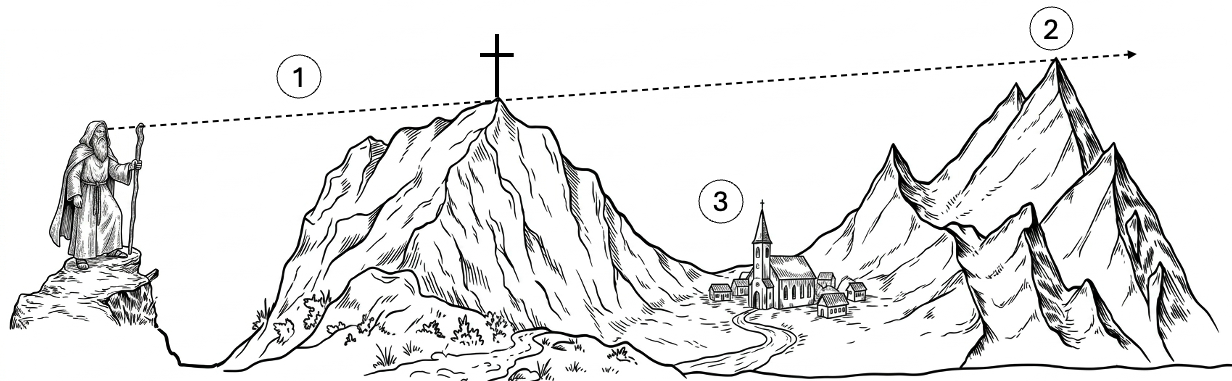
\includegraphics[
    width=1\textwidth, 
    trim=0 0 0 0, 
    clip]{images/mountain_peak_valley.png}
    \caption{「山峰觀」看「七十個七」}
    \label{fig:valley}
\end{figure}
}

\normalsize

圖 \ref{fig:valley}的
\ding{172}的期間是已經應驗的483年。\ding{173}是最後一個七，是先知所見的大災難七年。\ding{174}是山谷，是舊約先知們未見的奧秘，也就是教會的恩典時期。


為什麼山谷被隱藏？保羅說，教會是「奧秘」，「這奧秘在以前的世代、沒有叫人知道、像如今藉著聖靈啟示他的聖使徒和先知一樣．」（以弗所書3:5） 以及「這道理就是歷世歷代所隱藏的奧秘、但如今向他的聖徒顯明了．」（歌羅西書1:26）\footnote{更清楚的例子，是主耶穌在拿撒勒會堂讀以賽亞書61章，讀到「報告神悅納人的禧年」就停下來，把書捲起，說：「今天這經應驗在你們耳中了。」祂沒有讀下一句「和我們神報仇的日子」。在以賽亞書裡，這兩句只隔著一個逗號。在歷史上，卻已經相隔至少兩千年。（以賽亞書61:1-2與路加福音4:18-21）。因此，70個七中間有間隔的讀法並不是解經家憑空加上去的，而是與整本聖經預言一貫的寫法一致。}\footnote{並不是所有解經家都認為第69個七和第70個七之間有間隔。有些人（多屬無千禧年派或過去派）主張70個七是一段不間斷的490年。不過解經上時間對不上。造成更大的問題。在此因為已經超出本書範圍，不再贅述。}


\section*{七年的大災難：前三年半、後三年半}
經文還特別指出：「一七之半，他必使祭祀與供獻止息」，並設立「那行毀壞可憎的」。主耶穌在橄欖山講論中直接引用了這句話：「你們看見先知但以理所說的那行毀壞可憎的站在聖地……那時必有大災難」（馬太福音24:15、21）。由此可見，大災難總共七年，並以中間點為分水嶺。前三年半，敵基督假裝和平，與以色列立約。後三年半，他撕毀盟約，褻瀆聖殿，災難急劇加重，這就是狹義的「大災難」。

這三年半在聖經中有多種一致的說法：「一載二載半載」（ 1 + 2 + $\frac{1}{2}$ = 3 $\frac{1}{2}$）、「四十二個月」、「一千二百六十天」。這些經文互相印證，可見但以理所說的「一七」和「一七之半」都是確切的年日，不只是象徵。所以，大災難多久？按但以理書9章的框架，是七年，其中最嚴厲的「大災難」是後半段的三年半。
%\chapter*{附錄：何時被提}
%\phantomsection
%\addcontentsline{toc}{chapter}{附錄：何時被提}
%\markboth{附錄：何時被提}{附錄：何時被提}
%\setcounter{figure}{0}
%\renewcommand{\thefigure}{\arabic{figure}}   % this is the line that fixes \ref
%\def\theHfigure{appendix.\arabic{figure}}



%\appendix
\renewcommand{\appendixname}{附錄}
\renewcommand{\thechapter}{\arabic{chapter}}
\renewcommand{\thefigure}{\appendixname~\thechapter.\arabic{figure}}  % Appendix 1.1, 1.2, …

\refstepcounter{chapter}
\chapter*{附錄：何時被提}
\addcontentsline{toc}{chapter}%
  {\appendixname~\thechapter\quad 何時被提？}



\section*{什麼是「被提」（Rapture）？}


「被提」（Rapture）是指耶穌基督再來時，信徒被提到主那裡，與主相遇。主要根據是帖撒羅尼迦前書4:13–18，以及哥林多前書15:51–52等經文。

\begin{quote}

「論到睡了的人、我們不願意弟兄們不知道、恐怕你們憂傷、像那些沒有指望的人一樣。
我們若信耶穌死而復活了、那已經在耶穌裡睡了的人、　神也必將他與耶穌一同帶來。
我們現在照主的話告訴你們一件事．我們這活著還存留到主降臨的人、斷不能在那已經睡了的人之先．
因為主必親自從天降臨、有呼叫的聲音、和天使長的聲音、又有　神的號吹響．那在基督裡死了的人必先復活。
以後我們這活著還存留的人、必和他們一同被提到雲裡、在空中與主相遇．這樣、我們就要和主永遠同在。
所以你們當用這些話彼此勸慰。」（帖撒羅尼迦前書4:13–18）
\end{quote}

\begin{quote}
「我如今把一件奧秘的事告訴你們．我們不是都要睡覺、乃是都要改變。
就在一霎時、眨眼之間、號筒末次吹響的時候．因號筒要響、死人要復活成為不朽壞的、我們也要改變。」（哥林多前書15:51–52）
\end{quote}

被提可以分為「災前」、「災中」、「災後」被提三種。新約並沒有一節經文直接說「大災難之前被提」。以下的解釋是解經家根據經文的推論。

\section*{災前被提（Pretribulation）}

因為新約多處應許信徒必蒙保守，脫離將來神的忿怒。災前被提的觀點認為，教會要在七年大災難開始之前被提。主要依據的經文如下：

\begin{itemize}
\item 帖撒羅尼迦前書1:10：「救我們脫離將來忿怒的耶穌。」
\item 帖撒羅尼迦前書5:9：「神不是預定我們受刑、乃是預定我們藉著我們主耶穌基督得救。」這裡的「刑」原文就是「忿怒」，而上下文（5:1–3）講的正是主的日子。
\item 羅馬書5:9：「我們……更要藉著他免去神的忿怒。」
\item 啟示錄3:10：「我必在普天下人受試煉的時候、保守你免去你的試煉。」「免去」原文是「保守脫離」，意思是不在那段時間之中，而不只是在其中被保守。
\item 路加福音21:36：「你們要時時警醒、常常祈求、使你們能逃避這一切要來的事、得以站立在人子面前。」
\end{itemize}

另外，在舊約也有許多的預表：
\begin{itemize}
\item 創世記5:24：以諾在洪水審判之前被神取去。
\item 創世記19:22：天使對羅得說：「你要速速的逃到那城、因為你還沒有到那裡、我不能作甚麼。」審判要等義人離開以後才會降下。
\end{itemize}

如圖\ref{fig:pretribulation}所示：\ding{172}教會時期、\ding{173}大患難前被提、\ding{174}與耶穌一同回到地面作王、\ding{175}大災難、\ding{176}千禧年、\ding{177}新天新地。
    
\begin{figure}[htbp]
    \centering
    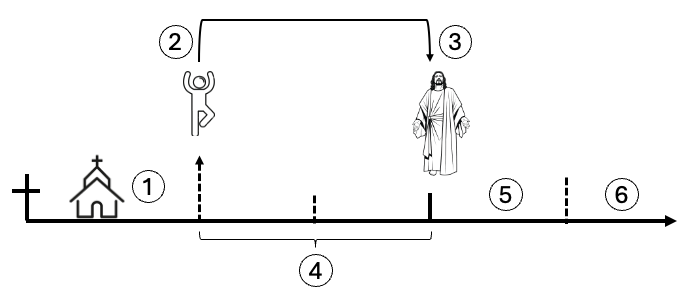
\includegraphics[
    width=1\textwidth, 
    trim=0 0 0 0, 
    clip]{images/pretribulation.png}
    \caption{災前被提}
    \label{fig:pretribulation}
\end{figure}




\section*{災中被提（Midtribulation）}

災中被提的觀點認為，教會要經過大災難的前三年半，在「一七之半」、神的忿怒傾倒之前被提，因為聖經把七年的中間點標示為轉折，而「末次的號筒」正在那時吹響：

\begin{itemize}
\item 但以理書9:27：「一七之半、他必使祭祀與供獻止息。」七年的中間點是整段時期的分水嶺。
\item 哥林多前書15:52：「號筒末次吹響的時候……我們也要改變。」災中被提派認為這「末次的號筒」就是啟示錄11:15的第七號。
\item 啟示錄11:11-12：兩個見證人傳道一千二百六十天（三年半）以後，聽見天上有聲音說：「上到這裡來。」他們就駕著雲上了天。這被視為信徒在災中被提的圖畫。
\item 啟示錄11:15、18：第七位天使吹號，天上說：「你的忿怒臨到了。」神的忿怒（七碗之災，啟16章）在後半段才傾倒。
\item 帖撒羅尼迦前書5:9：「神不是預定我們受刑」（原文「忿怒」）。災中被提派認為，前三年半是人和敵基督的逼迫，後三年半才是神的忿怒，信徒要在神的忿怒臨到之前被提。
\item 帖撒羅尼迦後書2:3-4：信徒被聚集之前，那大罪人要先「坐在神的殿裡、自稱是神」。這正是發生在七年中間的事（太24:15）。
\end{itemize}

如圖\ref{fig:midtribulation}所示：\ding{172}教會時期、\ding{173}大患難中被提、\ding{174}與耶穌一同回到地面作王、\ding{175}大災難、\ding{176}千禧年、\ding{177}新天新地。
\begin{figure}[htbp]
    \centering
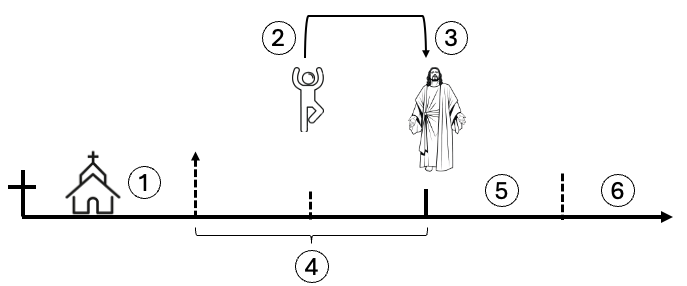
\includegraphics[
    width=1\textwidth, 
    trim=0 0 0 0, 
    clip]{images/midtribulation.png}
    \caption{災中被提}
    \label{fig:midtribulation}
\end{figure}

\section*{災後被提（Posttribulation）}

災後被提的觀點認為，教會要經過大災難，到災難結束、基督在榮耀中再來的時候，信徒才被提到空中與主相遇，因為新約描寫的「聚集選民」都在大災難之後：

\begin{itemize}
\item 馬太福音24:29-31：「那些日子的災難一過去……他要差遣使者、用號筒的大聲、將他的選民、從四方……都招聚了來。」主明說聚集選民是在災難之後。
\item 帖撒羅尼迦後書2:1-3：「論到我們主耶穌基督降臨、和我們到他那裡聚集……因為那日子以前、必有離道反教的事、並有那大罪人……顯露出來。」保羅說信徒被聚集之前，敵基督要先出現。
\item 帖撒羅尼迦後書1:6-7：「你們這受患難的人、與我們同得平安、那時主耶穌同他有能力的天使、從天上在火焰中顯現。」信徒得安息是在主公開顯現的時候。
\item 哥林多前書15:52：「號筒末次吹響的時候」，與馬太福音24:31的號筒，被認為是同一個時刻。
\item 啟示錄20:4-5：為耶穌作見證、沒有拜獸的人都復活了，「這是頭一次的復活」。如果「頭一次的復活」在大災難之後，信徒的復活和被提就也在災後。
\item 約翰福音17:15：「我不求你叫他們離開世界、只求你保守他們脫離那惡者。」神保守信徒的方式是在患難中保守，而不是把他們帶離患難。
\end{itemize}

另外，在舊約也有許多的預表：
\begin{itemize}
\item 創世記7:1、23：挪亞沒有在洪水以前被取去，而是在方舟裡經過洪水，蒙神保守。
\item 出埃及記8:22：神降災的時候，以色列人仍住在埃及，但神把歌珊地分別出來，災禍沒有臨到他們。
\end{itemize}

如圖\ref{fig:posttribulation}所示：\ding{172}教會時期、\ding{173}大患難後被提、\ding{174}與耶穌一同回到地面作王、\ding{175}大災難、\ding{176}千禧年、\ding{177}新天新地）。
\begin{figure}[htbp]
    \centering
    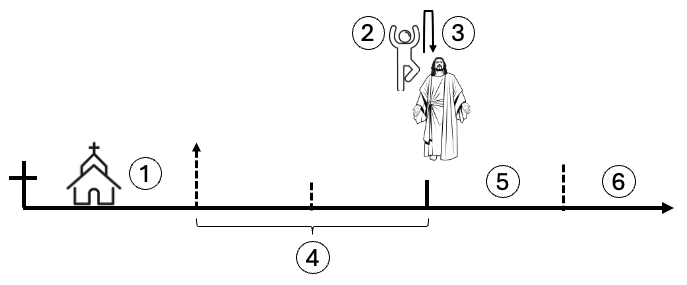
\includegraphics[
    width=1\textwidth, 
    trim=0 0 0 0, 
    clip]{images/posttribulation.png}
    \caption{災後被提}
    \label{fig:posttribulation}
\end{figure}



%\chapter*{附錄：千禧年觀}
%\phantomsection
%\addcontentsline{toc}{chapter}{附錄：千禧年觀}
%\markboth{附錄：千禧年觀}{附錄：千禧年觀}
%\setcounter{figure}{0}
%\renewcommand{\thefigure}{\arabic{figure}}   % this is the line that fixes \ref
%\def\theHfigure{appendix.\arabic{figure}}


%\appendix
\renewcommand{\appendixname}{附錄}
\renewcommand{\thechapter}{\arabic{chapter}}
\renewcommand{\thefigure}{\appendixname~\thechapter.\arabic{figure}}  % Appendix 1.1, 1.2, …

\refstepcounter{chapter}
\chapter*{附錄：千禧年觀}
\addcontentsline{toc}{chapter}%
  {\appendixname~\thechapter\quad 千禧年觀}




關於千禧年的解釋，大致可以分為前千禧年、後千禧年、無千禧年三種。我製作圖\ref{fig:premillennialism}、\ref{fig:postmillennialism}、\ref{fig:amillennialism} 來幫助我們了解。


\section*{前千禧年}
前千禧年的解釋，是\ding{172}教會時期，然後之後會有\ding{173}大患難時期。在大患難時期發生之前，\ding{174}耶穌再度降臨。大患難時期發生之後是\ding{175}千禧年，聖徒與耶穌一同作王，最後是\ding{176}新天新地。

\begin{figure}[htbp]
    \centering
    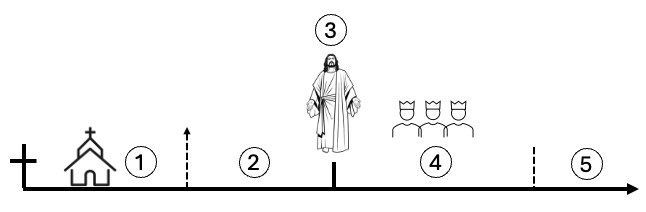
\includegraphics[width=\textwidth]{images/premillennialism.png}
    \caption{前千禧年觀}
    \label{fig:premillennialism}
\end{figure}

\section*{後千禧年}
後千禧年的解釋，是\ding{172}教會時期，然後是\ding{173}千禧年，然後\ding{174}耶穌再度降臨，最後是\ding{175}新天新地。 

\begin{figure}[htbp]
    \centering
    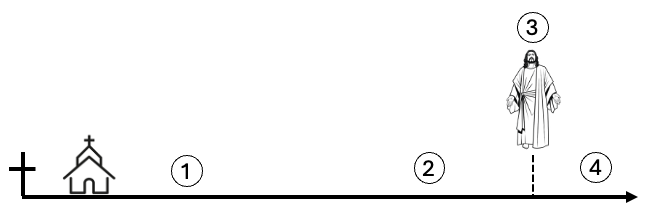
\includegraphics[width=\textwidth]{images/postmillennialism.png}
    \caption{後千禧年觀}
    \label{fig:postmillennialism}
\end{figure}

\section*{無千禧年}
無千禧年的解釋，是現在的\ding{172}教會時期就是千禧年，然後\ding{173}耶穌再度降臨，然後\ding{174}新天新地。 

\begin{figure}[htbp]
    \centering
    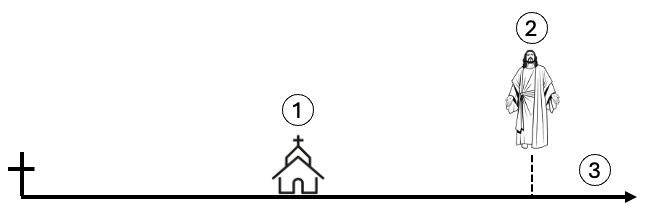
\includegraphics[width=\textwidth]{images/amillennialism.png}
    \caption{無千禧年觀}
    \label{fig:amillennialism}
\end{figure}


\begin{table}[htbp]
\centering
\small
\renewcommand{\arraystretch}{1.1}
\renewcommand{\thetable}{附錄\arabic{chapter}.\arabic{table}}% local to this table
\begin{minipage}{\linewidth}
\centering
\caption{三種千禧年觀的比較}\label{tab:millennium}
\begin{tabular}{p{0.12\linewidth}p{0.25\linewidth}p{0.25\linewidth}p{0.25\linewidth}}
\hline
列表 & 前千禧年觀 & 後千禧年觀 & 無千禧年觀 \\
\hline
英文 &
{\footnotesize Pre\-millennialism}\footnote{前千禧年論的代表人物：殉道者游斯丁（Justin Martyr）、愛任紐（Irenaeus）、特土良（Tertullian）、華富爾（John F. Walvoord）、萊里（Charles Ryrie）。} &
{\footnotesize Post\-millennialism}\footnote{後千禧年論的代表人物：愛德華滋（Jonathan Edwards）、賀智（Charles Hodge）、史普羅（R. C. Sproul）。} &
{\footnotesize A\-millennialism}\footnote{無千禧年論的代表人物：奧古斯丁（Augustine）、加爾文（John Calvin）、比爾（G. K. Beale）。} \\
基督再來 & 在千禧年之前 & 在千禧年之後 & 在千禧年（教會時代）之後 \\
千禧年 & 基督再來之後在地上實際統治1,000年 & 福音在世上大有能力的時期，帶來廣泛的歸信、公義與和平；通常理解為象徵性，而非字面上的一千年 & 教會時代，象徵性的「一千年」，即基督現今在天上的統治 \\
撒但被捆綁 & 千年完了暫時被釋放，然後被扔在火湖裡 & 大受限制，不能攔阻福音傳到萬國；捆綁發生在千禧年之前或期間 & 不能攔阻福音傳給萬國；但他並非毫無作為，仍繼續敵擋神的子民 \\
復活 & 兩個階段：信徒在千禧年之前或開始時復活；不信者在千禧年之後復活受審判 & 基督再來時，信與不信的人一次普遍復活 & 同後千禧年論 \\
最後叛亂 & 千禧年之後 & 千禧年將結束時 & 現今世代結束時 \\
\hline
\end{tabular}
\end{minipage}
\end{table}

%\chapter*{附錄：教師使用指南}
%\addcontentsline{toc}{chapter}{附錄：教師使用指南}

%\appendix
\renewcommand{\appendixname}{附錄}
\renewcommand{\thechapter}{\arabic{chapter}}
\renewcommand{\thefigure}{\appendixname~\thechapter.\arabic{figure}}  % Appendix 1.1, 1.2, …

\refstepcounter{chapter}
\chapter*{附錄：教師使用指南}
\addcontentsline{toc}{chapter}%
  {\appendixname~\thechapter\quad 教師使用指南}



此書適合成人主日學，或是小組研讀。以下建議進度表，方便教師或是帶領人安排進度。我的建議是採用八週作為主日學正式課程，並保留十週作為深入研讀版本。 

\section*{一、六週：掌握啟示錄的主線}

適合時間有限、希望在六週內掌握全書主要信息的班級。每週閱讀一個或數個相關章節，重點放在基督的身分、救贖、審判、得勝與新創造。
{
\renewcommand{\arraystretch}{1}
\begin{longtable}{
  >{\centering\arraybackslash}p{0.5cm}
  p{2cm}
  p{1cm}
  p{1.5cm}
  p{4cm}
}
週 &
主題 &
本書 &
啟示錄 &
教學重點 \\
\hline
\endfirsthead

週 &
主題 &
本書 &
啟示錄 &
教學重點 \\
\hline
\endhead

一 &
認識榮耀的基督與祂的教會 &
1-2 &
1-3 &
認識復活、掌權的基督；了解七教會的稱許、責備、命令與應許，思想教會如何忠心持守信仰。 \\

二 &
榮耀的寶座與羔羊展開書卷 &
3-4 &
4-5 &
從創造者的敬拜到被殺羔羊的敬拜，認識基督配得展開書卷，並掌管歷史。 \\

三 &
羔羊掌管歷史與審判 &
4-5 &
6-7 &
認識七印、四騎士、殉道者的呼求，以及受印的僕人和萬國萬民的敬拜；在苦難中持守盼望。 \\

四 &
基督審判世界，祂的百姓忠心作見證 &
5-6 &
8-11 &
認識七號的審判、兩個見證人和第七號，思想神的審判、憐憫與教會的見證使命。 \\

五 &
基督勝過龍、獸與巴比倫 &
7-10 &
12-19 &
認識龍、獸、假先知和巴比倫所代表的敵對勢力；思想聖徒如何靠羔羊得勝，並等候基督再來。 \\

六 &
基督擊敗撒但，神帶領百姓進入榮耀 &
11-12 &
20-22 &
認識千禧年不同觀點、最後審判、新天新地與新耶路撒冷；以「主耶穌啊，我願你來」作為課程的盼望與回應。 \\

\end{longtable}
}

\section*{二、八週：兼顧全書概覽與重要經文}

這是我最推薦的方案。每週可以安排約 60-75 分鐘，既能介紹啟示錄的主要異象，也能討論教會生活、苦難中的見證、末世觀點及基督徒的終極盼望。
{
\renewcommand{\arraystretch}{1}
\begin{longtable}{
  >{\centering\arraybackslash}p{0.5cm}
  p{2cm}
  p{1cm}
  p{1.5cm}
  p{4cm}
}
週 &
主題 &
本書 &
啟示錄 &
教學重點 \\
\hline
\endfirsthead

週 &
主題 &
本書 &
啟示錄 &
教學重點 \\
\hline
\endhead

一 &
認識榮耀的基督 &
1 &
1:1-20 &
了解約翰與拔摩島的背景；從基督的受苦、復活與掌權，認識啟示錄的中心人物。 \\

二 &
基督對祂的教會說話 &
2 &
2:1-3:22 &
研讀七教會的稱許、責備、命令與應許；思想教會如何悔改、持守真道，並忠心到底。 \\

三 &
榮耀的寶座與羔羊 &
3 &
4:1-5:14 &
從創造萬有的主到被殺的羔羊，認識天上敬拜的中心，以及基督為何配展開書卷。 \\

四 &
羔羊展開書卷 &
4 &
6:1-7:17 &
研讀七印、四騎士、殉道者、受印的僕人與萬國萬民的敬拜；思想苦難中的忍耐與救恩的盼望。 \\

五 &
基督審判世界，教會忠心作見證 &
5-6 &
8:1-11:19 &
研讀七號、兩個見證人和第七號；理解審判中的限制、人的不悔改，以及教會的見證使命。 \\

六 &
基督勝過龍與獸的權勢 &
7 &
12:1-14:20 &
了解婦人、男孩子、龍、海獸與假先知的象徵；思想聖徒如何靠羔羊的血和所見證的道得勝。 \\

七 &
公義審判與羔羊的得勝 &
8-10 &
15:1-19:21 &
研讀七碗、巴比倫傾倒、羔羊婚筵與騎白馬的基督；比較世界的權勢與基督最終的得勝。 \\

八 &
基督擊敗撒但，被恩典帶入榮耀 &
11-12 &
20:1-22:21 &
研讀千禧年、最後審判、新天新地與新耶路撒冷；認識不同末世觀點，並以盼望等候主再來。 \\

\end{longtable}
}


\section*{三、十週：深入研讀}

十週方案最能發揮本書的特色，尤其適合主日學教師培訓、成人查經班，以及希望進一步理解啟示錄象徵與末世觀點的讀者。

{
\renewcommand{\arraystretch}{1}
\begin{longtable}{
  >{\centering\arraybackslash}p{0.5cm}
  p{2cm}
  p{1cm}
  p{1.5cm}
  p{4cm}
}
週 &
主題 &
本書 &
啟示錄 &
教學重點 \\
\hline
\endfirsthead

週 &
主題 &
本書 &
啟示錄 &
教學重點 \\
\hline
\endhead

一 &
認識榮耀的基督 &
1 &
1:1-20 &
了解啟示錄的背景、約翰的見證，以及基督從受苦到得榮耀的身分；建立以基督為中心的閱讀方向。 \\

二 &
基督對祂的教會說話 &
2 &
2:1-3:22 &
逐一認識七教會；比較各教會的處境、優點、問題與應許，反思今日教會的信仰生活。 \\

三 &
榮耀的寶座與羔羊 &
3 &
4:1-5:14 &
研讀天上的寶座、四活物、二十四位長老與羔羊；理解創造與救贖如何匯合於敬拜。 \\

四 &
羔羊展開書卷 &
4 &
6:1-7:17 &
深入研讀七印、四騎士、殉道者的呼求、十四萬四千受印者與萬國萬民；比較七印的連續發生與重述觀點。 \\

五 &
七號與神的審判 &
5 &
8:1-9:21 &
研讀前六號及相關異象；注意「三分之一」所呈現的限制，並探討人為何在災難中仍不悔改。 \\

六 &
在苦難中忠心作見證 &
6 &
10:1-11:19 &
研讀小書卷、兩個見證人與第七號；理解神的話語、教會的見證，以及基督國度的宣告。 \\

七 &
基督勝過龍與獸的權勢 &
7 &
12:1-14:20 &
從婦人、男孩子、龍、兩個獸與十四萬四千人，認識屬靈爭戰、敵對神的權勢，以及聖徒的忠心。 \\

八 &
七碗、巴比倫與羔羊得勝 &
8-10 &
15:1-19:21 &
研讀七碗、巴比倫的傾倒、羔羊婚筵與基督再來；認識神的公義審判，以及世俗權勢終必敗亡。 \\

九 &
千禧年、撒但與最後審判 &
11 &
20:1-15 &
研讀撒但被捆綁、千禧年、歌革與瑪各，以及白色大寶座；比較前千禧年、無千禧年與後千禧年觀點。 \\

十 &
新天新地：被恩典帶入榮耀 &
12 &
21:1-22:21 &
研讀新耶路撒冷、神與人同住、生命河與生命樹；以新創造的盼望和「主耶穌啊，我願你來」作結。 \\

\end{longtable}

}
\clearpage
\thispagestyle{empty}
\mbox{}
\clearpage

\end{document}